
% Default to the notebook output style

    


% Inherit from the specified cell style.




    
\documentclass{article}

    
    
    \usepackage{graphicx} % Used to insert images
    \usepackage{adjustbox} % Used to constrain images to a maximum size 
    \usepackage{color} % Allow colors to be defined
    \usepackage{enumerate} % Needed for markdown enumerations to work
    \usepackage{geometry} % Used to adjust the document margins
    \usepackage{amsmath} % Equations
    \usepackage{amssymb} % Equations
    \usepackage{eurosym} % defines \euro
    \usepackage[mathletters]{ucs} % Extended unicode (utf-8) support
    \usepackage[utf8x]{inputenc} % Allow utf-8 characters in the tex document
    \usepackage{fancyvrb} % verbatim replacement that allows latex
    \usepackage{grffile} % extends the file name processing of package graphics 
                         % to support a larger range 
    % The hyperref package gives us a pdf with properly built
    % internal navigation ('pdf bookmarks' for the table of contents,
    % internal cross-reference links, web links for URLs, etc.)
    \usepackage{hyperref}
    \usepackage{longtable} % longtable support required by pandoc >1.10
    \usepackage{booktabs}  % table support for pandoc > 1.12.2
    \usepackage{ulem} % ulem is needed to support strikethroughs (\sout)
    \usepackage{natbib}
    

    
    
    \definecolor{orange}{cmyk}{0,0.4,0.8,0.2}
    \definecolor{darkorange}{rgb}{.71,0.21,0.01}
    \definecolor{darkgreen}{rgb}{.12,.54,.11}
    \definecolor{myteal}{rgb}{.26, .44, .56}
    \definecolor{gray}{gray}{0.45}
    \definecolor{lightgray}{gray}{.95}
    \definecolor{mediumgray}{gray}{.8}
    \definecolor{inputbackground}{rgb}{.95, .95, .85}
    \definecolor{outputbackground}{rgb}{.95, .95, .95}
    \definecolor{traceback}{rgb}{1, .95, .95}
    % ansi colors
    \definecolor{red}{rgb}{.6,0,0}
    \definecolor{green}{rgb}{0,.65,0}
    \definecolor{brown}{rgb}{0.6,0.6,0}
    \definecolor{blue}{rgb}{0,.145,.698}
    \definecolor{purple}{rgb}{.698,.145,.698}
    \definecolor{cyan}{rgb}{0,.698,.698}
    \definecolor{lightgray}{gray}{0.5}
    
    % bright ansi colors
    \definecolor{darkgray}{gray}{0.25}
    \definecolor{lightred}{rgb}{1.0,0.39,0.28}
    \definecolor{lightgreen}{rgb}{0.48,0.99,0.0}
    \definecolor{lightblue}{rgb}{0.53,0.81,0.92}
    \definecolor{lightpurple}{rgb}{0.87,0.63,0.87}
    \definecolor{lightcyan}{rgb}{0.5,1.0,0.83}
    
    % commands and environments needed by pandoc snippets
    % extracted from the output of `pandoc -s`
    \providecommand{\tightlist}{%
      \setlength{\itemsep}{0pt}\setlength{\parskip}{0pt}}
    \DefineVerbatimEnvironment{Highlighting}{Verbatim}{commandchars=\\\{\}}
    % Add ',fontsize=\small' for more characters per line
    \newenvironment{Shaded}{}{}
    \newcommand{\KeywordTok}[1]{\textcolor[rgb]{0.00,0.44,0.13}{\textbf{{#1}}}}
    \newcommand{\DataTypeTok}[1]{\textcolor[rgb]{0.56,0.13,0.00}{{#1}}}
    \newcommand{\DecValTok}[1]{\textcolor[rgb]{0.25,0.63,0.44}{{#1}}}
    \newcommand{\BaseNTok}[1]{\textcolor[rgb]{0.25,0.63,0.44}{{#1}}}
    \newcommand{\FloatTok}[1]{\textcolor[rgb]{0.25,0.63,0.44}{{#1}}}
    \newcommand{\CharTok}[1]{\textcolor[rgb]{0.25,0.44,0.63}{{#1}}}
    \newcommand{\StringTok}[1]{\textcolor[rgb]{0.25,0.44,0.63}{{#1}}}
    \newcommand{\CommentTok}[1]{\textcolor[rgb]{0.38,0.63,0.69}{\textit{{#1}}}}
    \newcommand{\OtherTok}[1]{\textcolor[rgb]{0.00,0.44,0.13}{{#1}}}
    \newcommand{\AlertTok}[1]{\textcolor[rgb]{1.00,0.00,0.00}{\textbf{{#1}}}}
    \newcommand{\FunctionTok}[1]{\textcolor[rgb]{0.02,0.16,0.49}{{#1}}}
    \newcommand{\RegionMarkerTok}[1]{{#1}}
    \newcommand{\ErrorTok}[1]{\textcolor[rgb]{1.00,0.00,0.00}{\textbf{{#1}}}}
    \newcommand{\NormalTok}[1]{{#1}}
    
    % Additional commands for more recent versions of Pandoc
    \newcommand{\ConstantTok}[1]{\textcolor[rgb]{0.53,0.00,0.00}{{#1}}}
    \newcommand{\SpecialCharTok}[1]{\textcolor[rgb]{0.25,0.44,0.63}{{#1}}}
    \newcommand{\VerbatimStringTok}[1]{\textcolor[rgb]{0.25,0.44,0.63}{{#1}}}
    \newcommand{\SpecialStringTok}[1]{\textcolor[rgb]{0.73,0.40,0.53}{{#1}}}
    \newcommand{\ImportTok}[1]{{#1}}
    \newcommand{\DocumentationTok}[1]{\textcolor[rgb]{0.73,0.13,0.13}{\textit{{#1}}}}
    \newcommand{\AnnotationTok}[1]{\textcolor[rgb]{0.38,0.63,0.69}{\textbf{\textit{{#1}}}}}
    \newcommand{\CommentVarTok}[1]{\textcolor[rgb]{0.38,0.63,0.69}{\textbf{\textit{{#1}}}}}
    \newcommand{\VariableTok}[1]{\textcolor[rgb]{0.10,0.09,0.49}{{#1}}}
    \newcommand{\ControlFlowTok}[1]{\textcolor[rgb]{0.00,0.44,0.13}{\textbf{{#1}}}}
    \newcommand{\OperatorTok}[1]{\textcolor[rgb]{0.40,0.40,0.40}{{#1}}}
    \newcommand{\BuiltInTok}[1]{{#1}}
    \newcommand{\ExtensionTok}[1]{{#1}}
    \newcommand{\PreprocessorTok}[1]{\textcolor[rgb]{0.74,0.48,0.00}{{#1}}}
    \newcommand{\AttributeTok}[1]{\textcolor[rgb]{0.49,0.56,0.16}{{#1}}}
    \newcommand{\InformationTok}[1]{\textcolor[rgb]{0.38,0.63,0.69}{\textbf{\textit{{#1}}}}}
    \newcommand{\WarningTok}[1]{\textcolor[rgb]{0.38,0.63,0.69}{\textbf{\textit{{#1}}}}}
    
    
    % Define a nice break command that doesn't care if a line doesn't already
    % exist.
    \def\br{\hspace*{\fill} \\* }
    % Math Jax compatability definitions
    \def\gt{>}
    \def\lt{<}
    % Document parameters
    \title{Data repository for ``The end of Midcontinent Rift magmatism and the paleogeography of Laurentia''}
    \date{}
    
    \renewcommand{\refname}{}
    
    
    

    % Pygments definitions
    
\makeatletter
\def\PY@reset{\let\PY@it=\relax \let\PY@bf=\relax%
    \let\PY@ul=\relax \let\PY@tc=\relax%
    \let\PY@bc=\relax \let\PY@ff=\relax}
\def\PY@tok#1{\csname PY@tok@#1\endcsname}
\def\PY@toks#1+{\ifx\relax#1\empty\else%
    \PY@tok{#1}\expandafter\PY@toks\fi}
\def\PY@do#1{\PY@bc{\PY@tc{\PY@ul{%
    \PY@it{\PY@bf{\PY@ff{#1}}}}}}}
\def\PY#1#2{\PY@reset\PY@toks#1+\relax+\PY@do{#2}}

\expandafter\def\csname PY@tok@vg\endcsname{\def\PY@tc##1{\textcolor[rgb]{0.10,0.09,0.49}{##1}}}
\expandafter\def\csname PY@tok@s\endcsname{\def\PY@tc##1{\textcolor[rgb]{0.73,0.13,0.13}{##1}}}
\expandafter\def\csname PY@tok@vc\endcsname{\def\PY@tc##1{\textcolor[rgb]{0.10,0.09,0.49}{##1}}}
\expandafter\def\csname PY@tok@kn\endcsname{\let\PY@bf=\textbf\def\PY@tc##1{\textcolor[rgb]{0.00,0.50,0.00}{##1}}}
\expandafter\def\csname PY@tok@ow\endcsname{\let\PY@bf=\textbf\def\PY@tc##1{\textcolor[rgb]{0.67,0.13,1.00}{##1}}}
\expandafter\def\csname PY@tok@nd\endcsname{\def\PY@tc##1{\textcolor[rgb]{0.67,0.13,1.00}{##1}}}
\expandafter\def\csname PY@tok@c\endcsname{\let\PY@it=\textit\def\PY@tc##1{\textcolor[rgb]{0.25,0.50,0.50}{##1}}}
\expandafter\def\csname PY@tok@si\endcsname{\let\PY@bf=\textbf\def\PY@tc##1{\textcolor[rgb]{0.73,0.40,0.53}{##1}}}
\expandafter\def\csname PY@tok@err\endcsname{\def\PY@bc##1{\setlength{\fboxsep}{0pt}\fcolorbox[rgb]{1.00,0.00,0.00}{1,1,1}{\strut ##1}}}
\expandafter\def\csname PY@tok@gi\endcsname{\def\PY@tc##1{\textcolor[rgb]{0.00,0.63,0.00}{##1}}}
\expandafter\def\csname PY@tok@mb\endcsname{\def\PY@tc##1{\textcolor[rgb]{0.40,0.40,0.40}{##1}}}
\expandafter\def\csname PY@tok@ss\endcsname{\def\PY@tc##1{\textcolor[rgb]{0.10,0.09,0.49}{##1}}}
\expandafter\def\csname PY@tok@gd\endcsname{\def\PY@tc##1{\textcolor[rgb]{0.63,0.00,0.00}{##1}}}
\expandafter\def\csname PY@tok@mi\endcsname{\def\PY@tc##1{\textcolor[rgb]{0.40,0.40,0.40}{##1}}}
\expandafter\def\csname PY@tok@bp\endcsname{\def\PY@tc##1{\textcolor[rgb]{0.00,0.50,0.00}{##1}}}
\expandafter\def\csname PY@tok@mh\endcsname{\def\PY@tc##1{\textcolor[rgb]{0.40,0.40,0.40}{##1}}}
\expandafter\def\csname PY@tok@gp\endcsname{\let\PY@bf=\textbf\def\PY@tc##1{\textcolor[rgb]{0.00,0.00,0.50}{##1}}}
\expandafter\def\csname PY@tok@m\endcsname{\def\PY@tc##1{\textcolor[rgb]{0.40,0.40,0.40}{##1}}}
\expandafter\def\csname PY@tok@s2\endcsname{\def\PY@tc##1{\textcolor[rgb]{0.73,0.13,0.13}{##1}}}
\expandafter\def\csname PY@tok@kc\endcsname{\let\PY@bf=\textbf\def\PY@tc##1{\textcolor[rgb]{0.00,0.50,0.00}{##1}}}
\expandafter\def\csname PY@tok@gu\endcsname{\let\PY@bf=\textbf\def\PY@tc##1{\textcolor[rgb]{0.50,0.00,0.50}{##1}}}
\expandafter\def\csname PY@tok@sd\endcsname{\let\PY@it=\textit\def\PY@tc##1{\textcolor[rgb]{0.73,0.13,0.13}{##1}}}
\expandafter\def\csname PY@tok@w\endcsname{\def\PY@tc##1{\textcolor[rgb]{0.73,0.73,0.73}{##1}}}
\expandafter\def\csname PY@tok@ch\endcsname{\let\PY@it=\textit\def\PY@tc##1{\textcolor[rgb]{0.25,0.50,0.50}{##1}}}
\expandafter\def\csname PY@tok@cs\endcsname{\let\PY@it=\textit\def\PY@tc##1{\textcolor[rgb]{0.25,0.50,0.50}{##1}}}
\expandafter\def\csname PY@tok@nc\endcsname{\let\PY@bf=\textbf\def\PY@tc##1{\textcolor[rgb]{0.00,0.00,1.00}{##1}}}
\expandafter\def\csname PY@tok@gs\endcsname{\let\PY@bf=\textbf}
\expandafter\def\csname PY@tok@na\endcsname{\def\PY@tc##1{\textcolor[rgb]{0.49,0.56,0.16}{##1}}}
\expandafter\def\csname PY@tok@ne\endcsname{\let\PY@bf=\textbf\def\PY@tc##1{\textcolor[rgb]{0.82,0.25,0.23}{##1}}}
\expandafter\def\csname PY@tok@gr\endcsname{\def\PY@tc##1{\textcolor[rgb]{1.00,0.00,0.00}{##1}}}
\expandafter\def\csname PY@tok@kp\endcsname{\def\PY@tc##1{\textcolor[rgb]{0.00,0.50,0.00}{##1}}}
\expandafter\def\csname PY@tok@se\endcsname{\let\PY@bf=\textbf\def\PY@tc##1{\textcolor[rgb]{0.73,0.40,0.13}{##1}}}
\expandafter\def\csname PY@tok@ni\endcsname{\let\PY@bf=\textbf\def\PY@tc##1{\textcolor[rgb]{0.60,0.60,0.60}{##1}}}
\expandafter\def\csname PY@tok@no\endcsname{\def\PY@tc##1{\textcolor[rgb]{0.53,0.00,0.00}{##1}}}
\expandafter\def\csname PY@tok@gt\endcsname{\def\PY@tc##1{\textcolor[rgb]{0.00,0.27,0.87}{##1}}}
\expandafter\def\csname PY@tok@kt\endcsname{\def\PY@tc##1{\textcolor[rgb]{0.69,0.00,0.25}{##1}}}
\expandafter\def\csname PY@tok@nf\endcsname{\def\PY@tc##1{\textcolor[rgb]{0.00,0.00,1.00}{##1}}}
\expandafter\def\csname PY@tok@il\endcsname{\def\PY@tc##1{\textcolor[rgb]{0.40,0.40,0.40}{##1}}}
\expandafter\def\csname PY@tok@mo\endcsname{\def\PY@tc##1{\textcolor[rgb]{0.40,0.40,0.40}{##1}}}
\expandafter\def\csname PY@tok@nt\endcsname{\let\PY@bf=\textbf\def\PY@tc##1{\textcolor[rgb]{0.00,0.50,0.00}{##1}}}
\expandafter\def\csname PY@tok@c1\endcsname{\let\PY@it=\textit\def\PY@tc##1{\textcolor[rgb]{0.25,0.50,0.50}{##1}}}
\expandafter\def\csname PY@tok@nv\endcsname{\def\PY@tc##1{\textcolor[rgb]{0.10,0.09,0.49}{##1}}}
\expandafter\def\csname PY@tok@s1\endcsname{\def\PY@tc##1{\textcolor[rgb]{0.73,0.13,0.13}{##1}}}
\expandafter\def\csname PY@tok@cpf\endcsname{\let\PY@it=\textit\def\PY@tc##1{\textcolor[rgb]{0.25,0.50,0.50}{##1}}}
\expandafter\def\csname PY@tok@o\endcsname{\def\PY@tc##1{\textcolor[rgb]{0.40,0.40,0.40}{##1}}}
\expandafter\def\csname PY@tok@gh\endcsname{\let\PY@bf=\textbf\def\PY@tc##1{\textcolor[rgb]{0.00,0.00,0.50}{##1}}}
\expandafter\def\csname PY@tok@sh\endcsname{\def\PY@tc##1{\textcolor[rgb]{0.73,0.13,0.13}{##1}}}
\expandafter\def\csname PY@tok@sx\endcsname{\def\PY@tc##1{\textcolor[rgb]{0.00,0.50,0.00}{##1}}}
\expandafter\def\csname PY@tok@kr\endcsname{\let\PY@bf=\textbf\def\PY@tc##1{\textcolor[rgb]{0.00,0.50,0.00}{##1}}}
\expandafter\def\csname PY@tok@cp\endcsname{\def\PY@tc##1{\textcolor[rgb]{0.74,0.48,0.00}{##1}}}
\expandafter\def\csname PY@tok@mf\endcsname{\def\PY@tc##1{\textcolor[rgb]{0.40,0.40,0.40}{##1}}}
\expandafter\def\csname PY@tok@k\endcsname{\let\PY@bf=\textbf\def\PY@tc##1{\textcolor[rgb]{0.00,0.50,0.00}{##1}}}
\expandafter\def\csname PY@tok@vi\endcsname{\def\PY@tc##1{\textcolor[rgb]{0.10,0.09,0.49}{##1}}}
\expandafter\def\csname PY@tok@sr\endcsname{\def\PY@tc##1{\textcolor[rgb]{0.73,0.40,0.53}{##1}}}
\expandafter\def\csname PY@tok@nn\endcsname{\let\PY@bf=\textbf\def\PY@tc##1{\textcolor[rgb]{0.00,0.00,1.00}{##1}}}
\expandafter\def\csname PY@tok@go\endcsname{\def\PY@tc##1{\textcolor[rgb]{0.53,0.53,0.53}{##1}}}
\expandafter\def\csname PY@tok@nl\endcsname{\def\PY@tc##1{\textcolor[rgb]{0.63,0.63,0.00}{##1}}}
\expandafter\def\csname PY@tok@nb\endcsname{\def\PY@tc##1{\textcolor[rgb]{0.00,0.50,0.00}{##1}}}
\expandafter\def\csname PY@tok@ge\endcsname{\let\PY@it=\textit}
\expandafter\def\csname PY@tok@sb\endcsname{\def\PY@tc##1{\textcolor[rgb]{0.73,0.13,0.13}{##1}}}
\expandafter\def\csname PY@tok@sc\endcsname{\def\PY@tc##1{\textcolor[rgb]{0.73,0.13,0.13}{##1}}}
\expandafter\def\csname PY@tok@cm\endcsname{\let\PY@it=\textit\def\PY@tc##1{\textcolor[rgb]{0.25,0.50,0.50}{##1}}}
\expandafter\def\csname PY@tok@kd\endcsname{\let\PY@bf=\textbf\def\PY@tc##1{\textcolor[rgb]{0.00,0.50,0.00}{##1}}}

\def\PYZbs{\char`\\}
\def\PYZus{\char`\_}
\def\PYZob{\char`\{}
\def\PYZcb{\char`\}}
\def\PYZca{\char`\^}
\def\PYZam{\char`\&}
\def\PYZlt{\char`\<}
\def\PYZgt{\char`\>}
\def\PYZsh{\char`\#}
\def\PYZpc{\char`\%}
\def\PYZdl{\char`\$}
\def\PYZhy{\char`\-}
\def\PYZsq{\char`\'}
\def\PYZdq{\char`\"}
\def\PYZti{\char`\~}
% for compatibility with earlier versions
\def\PYZat{@}
\def\PYZlb{[}
\def\PYZrb{]}
\makeatother


    % Exact colors from NB
    \definecolor{incolor}{rgb}{0.0, 0.0, 0.5}
    \definecolor{outcolor}{rgb}{0.545, 0.0, 0.0}



    
    % Prevent overflowing lines due to hard-to-break entities
    \sloppy 
    % Setup hyperref package
    \hypersetup{
      breaklinks=true,  % so long urls are correctly broken across lines
      colorlinks=true,
      urlcolor=blue,
      linkcolor=darkorange,
      citecolor=darkgreen,
      }
    % Slightly bigger margins than the latex defaults
    
    \geometry{verbose,tmargin=1in,bmargin=1in,lmargin=1in,rmargin=1in}
    
    

    \begin{document}
    
    
    \maketitle
    
    

    
\label{paleomagnetic-data-analysis-of-late-stage-volcanics-from-the-midcontinent-rift}

\noindent This Jupyter notebook is provided as Data Repository materials for:
\begin{quote}
Fairchild, L.M., Swanson-Hysell, N.L., Ramenzani, J., Sprain, C.J., and Bowring, S.A. The end of Midcontinent Rift magmatism and the paleogeography of Laurentia. Lithosphere, doi:10.1130/L580.1.
\end{quote}
This notebook contains the code (written in Python 2.7) used for data analysis and figure generation for this study. This notebook can be \href{https://github.com/Swanson-Hysell-Group/2016_Late_Rift/blob/master/Code/Late_Rift_Data_Analysis.ipynb}{downloaded for interactive viewing}\footnotemark\ or \href{https://nbviewer.jupyter.org/github/swanson-hysell-group/2016_Late_Rift/blob/master/Code/Late_Rift_Data_Analysis.ipynb}{viewed statically within a web browser}\footnotemark . These ways of viewing the notebook are preferable although a PDF rendering of the notebook is provided in the GSA Data Repository.\\

\footnoterule

\noindent\footnotemark[1]\texttt{\scriptsize{https://github.com/Swanson-Hysell-Group/2016\_Late\_Rift/blob/master/Code/Late\_Rift\_Data\_Analysis.ipynb}}
\footnotemark[2]\texttt{\scriptsize{https://nbviewer.jupyter.org/github/swanson-hysell-group/2016\_Late\_Rift/blob/master/Code/Late\_Rift\_Data\_Analysis.ipynb}}

\tableofcontents{}

\section{Import and develop functions for use within the Jupyter notebook}\label{import-and-develop-functions-for-use-within-the-jupyter-notebook}
The next three code blocks import necessary libraries and define functions
that will be used in the data analysis below. The modules
\texttt{pmag.py}, \texttt{pmagplotlib.py} and \texttt{ipmag.py} are from
the PmagPy software package (https://github.com/ltauxe/PmagPy; \citealp{Tauxe2016a}). The
current version of these modules (PmagPy 3.4) are included in the Github
repository with this notebook. Other necessary function libraries
(\texttt{matplotlib}, \texttt{pandas}, \texttt{Basemap},
\texttt{IPython}, \texttt{numpy}, \texttt{scipy}) are included with
standard scientific Python distributions.


    \begin{Verbatim}[commandchars=\\\{\}]
{\color{incolor}In [{\color{incolor}1}]:} \PY{k+kn}{import} \PY{n+nn}{pmagpy\PYZus{}3\PYZus{}4.pmag} \PY{k+kn}{as} \PY{n+nn}{pmag}
        \PY{k+kn}{import} \PY{n+nn}{pmagpy\PYZus{}3\PYZus{}4.pmagplotlib} \PY{k+kn}{as} \PY{n+nn}{pmagplotlib}
        \PY{k+kn}{import} \PY{n+nn}{pmagpy\PYZus{}3\PYZus{}4.ipmag} \PY{k+kn}{as} \PY{n+nn}{ipmag}
        
        \PY{k+kn}{import} \PY{n+nn}{matplotlib.pyplot} \PY{k+kn}{as} \PY{n+nn}{plt}
        \PY{k+kn}{from} \PY{n+nn}{mpl\PYZus{}toolkits.basemap} \PY{k+kn}{import} \PY{n}{Basemap}
        \PY{k+kn}{from} \PY{n+nn}{matplotlib.patches} \PY{k+kn}{import} \PY{n}{Polygon}
        \PY{k+kn}{import} \PY{n+nn}{matplotlib.patches} \PY{k+kn}{as} \PY{n+nn}{mpatch}
        \PY{k+kn}{from} \PY{n+nn}{matplotlib.collections} \PY{k+kn}{import} \PY{n}{PatchCollection}
        \PY{k+kn}{import} \PY{n+nn}{pandas} \PY{k+kn}{as} \PY{n+nn}{pd}
        \PY{k+kn}{from} \PY{n+nn}{IPython.core.display} \PY{k+kn}{import} \PY{n}{HTML}
        \PY{k+kn}{import} \PY{n+nn}{numpy} \PY{k+kn}{as} \PY{n+nn}{np}
        \PY{k+kn}{import} \PY{n+nn}{scipy} \PY{k+kn}{as} \PY{n+nn}{sp}
        \PY{k+kn}{from} \PY{n+nn}{scipy} \PY{k+kn}{import} \PY{n}{special}
        \PY{k+kn}{from} \PY{n+nn}{IPython.display} \PY{k+kn}{import} \PY{n}{Image}
\end{Verbatim}
This notebook runs with figures inline in the Jupyter notebook (instead of opening up in another window) by executing this command:

    \begin{Verbatim}[commandchars=\\\{\}]
{\color{incolor}In [{\color{incolor}2}]:} \PY{o}{\PYZpc{}}\PY{k}{matplotlib} inline
        \PY{o}{\PYZpc{}}\PY{k}{config} InlineBackend.figure\PYZus{}formats = \PYZob{}\PYZsq{}svg\PYZsq{},\PYZcb{}
\end{Verbatim}
Throughout this analysis there will be maps that show pole positions. The \texttt{pole\_figure\_appearance} function controls aspects of the appearance
of these maps and eliminates the need to make these customizations for
every plot.

    \begin{Verbatim}[commandchars=\\\{\}]
{\color{incolor}In [{\color{incolor}3}]:} \PY{k}{def} \PY{n+nf}{pole\PYZus{}figure\PYZus{}appearance}\PY{p}{(}\PY{n}{size} \PY{o}{=} \PY{p}{(}\PY{l+m+mi}{7}\PY{p}{,}\PY{l+m+mi}{7}\PY{p}{)}\PY{p}{)}\PY{p}{:}
            \PY{n}{m} \PY{o}{=} \PY{n}{Basemap}\PY{p}{(}\PY{n}{projection}\PY{o}{=}\PY{l+s+s1}{\PYZsq{}}\PY{l+s+s1}{ortho}\PY{l+s+s1}{\PYZsq{}}\PY{p}{,}\PY{n}{lat\PYZus{}0}\PY{o}{=}\PY{l+m+mi}{35}\PY{p}{,}\PY{n}{lon\PYZus{}0}\PY{o}{=}\PY{l+m+mi}{200}\PY{p}{,}\PY{n}{resolution}\PY{o}{=}\PY{l+s+s1}{\PYZsq{}}\PY{l+s+s1}{c}\PY{l+s+s1}{\PYZsq{}}\PY{p}{,}
                        \PY{n}{area\PYZus{}thresh}\PY{o}{=}\PY{l+m+mi}{50000}\PY{p}{)}
            \PY{n}{plt}\PY{o}{.}\PY{n}{figure}\PY{p}{(}\PY{n}{figsize}\PY{o}{=}\PY{n}{size}\PY{p}{)}
            \PY{n}{m}\PY{o}{.}\PY{n}{drawcoastlines}\PY{p}{(}\PY{n}{linewidth}\PY{o}{=}\PY{l+m+mf}{0.25}\PY{p}{)}
            \PY{n}{m}\PY{o}{.}\PY{n}{fillcontinents}\PY{p}{(}\PY{n}{color}\PY{o}{=}\PY{l+s+s1}{\PYZsq{}}\PY{l+s+s1}{bisque}\PY{l+s+s1}{\PYZsq{}}\PY{p}{,}\PY{n}{lake\PYZus{}color}\PY{o}{=}\PY{l+s+s1}{\PYZsq{}}\PY{l+s+s1}{white}\PY{l+s+s1}{\PYZsq{}}\PY{p}{,}\PY{n}{zorder}\PY{o}{=}\PY{l+m+mi}{1}\PY{p}{)}
            \PY{n}{m}\PY{o}{.}\PY{n}{drawmapboundary}\PY{p}{(}\PY{n}{fill\PYZus{}color}\PY{o}{=}\PY{l+s+s1}{\PYZsq{}}\PY{l+s+s1}{white}\PY{l+s+s1}{\PYZsq{}}\PY{p}{)}
            \PY{n}{m}\PY{o}{.}\PY{n}{drawmeridians}\PY{p}{(}\PY{n}{np}\PY{o}{.}\PY{n}{arange}\PY{p}{(}\PY{l+m+mi}{0}\PY{p}{,}\PY{l+m+mi}{360}\PY{p}{,}\PY{l+m+mi}{30}\PY{p}{)}\PY{p}{)}
            \PY{n}{m}\PY{o}{.}\PY{n}{drawparallels}\PY{p}{(}\PY{n}{np}\PY{o}{.}\PY{n}{arange}\PY{p}{(}\PY{o}{\PYZhy{}}\PY{l+m+mi}{90}\PY{p}{,}\PY{l+m+mi}{90}\PY{p}{,}\PY{l+m+mi}{30}\PY{p}{)}\PY{p}{)}
            \PY{k}{return} \PY{n}{m}
\end{Verbatim}

\section{Schroeder-Lutsen Basalts}\label{schroeder-lutsen-basalts}

\subsection{Prior data}\label{prior-data}

\cite{Tauxe2009a} published data from sites of the North Shore
Volcanic Group and Schroeder-Lutsen Basalts that was the first study of
these units to use modern methods. \cite{Books1968a,Books1972a} and \cite{Palmer1970a}
also developed data that can largely be considered to be superseded by
the Tauxe and Kodama results. In the code below, the \cite{Tauxe2009a} data are imported and then the data that are from the
Schroeder-Lutsen Basalts are split off from the rest of the data from the North Shore Volcanic
Group.

    \begin{Verbatim}[commandchars=\\\{\}]
{\color{incolor}In [{\color{incolor}4}]:} \PY{n}{Tauxe\PYZus{}NSVG\PYZus{}Data}\PY{o}{=}\PY{n}{pd}\PY{o}{.}\PY{n}{read\PYZus{}csv}\PY{p}{(}\PY{l+s+s1}{\PYZsq{}}\PY{l+s+s1}{../Data/Previous\PYZus{}studies/Tauxe2009a\PYZus{}data.csv}\PY{l+s+s1}{\PYZsq{}}\PY{p}{,}\PY{n}{sep}\PY{o}{=}\PY{l+s+s1}{\PYZsq{}}\PY{l+s+s1}{,}\PY{l+s+s1}{\PYZsq{}}\PY{p}{)}
        \PY{n}{Tauxe\PYZus{}NSVG\PYZus{}Data}\PY{o}{.}\PY{n}{head}\PY{p}{(}\PY{p}{)}
\end{Verbatim}

            \begin{Verbatim}[commandchars=\\\{\}]
{\color{outcolor}Out[{\color{outcolor}4}]:}   \href{http://earthref.org/MagIC/8407/}{MagIC contribution of Tauxe and Kodama (2009)} (http://earthref.org/MagIC/8407/)
\end{Verbatim}
\noindent \textbf{NOTE: }If you are having trouble opening the above link to the MagIC database, the file can also be found in the Github repository under \texttt{/Data/Previous\_studies/Tauxe2009a\_data.csv}.\\  
        
The \textbf{sequence} column contains an assignment of the sequence with
`nsl' signifying that we interpret to be flows within the
Schroeder-Lutsen basalts. A new dataframe can be made with only these
flows.

    \begin{Verbatim}[commandchars=\\\{\}]
{\color{incolor}In [{\color{incolor}5}]:} \PY{n}{NSVG\PYZus{}nswu} \PY{o}{=} \PY{n}{Tauxe\PYZus{}NSVG\PYZus{}Data}\PY{o}{.}\PY{n}{ix}\PY{p}{[}\PY{n}{Tauxe\PYZus{}NSVG\PYZus{}Data}\PY{p}{[}\PY{l+s+s1}{\PYZsq{}}\PY{l+s+s1}{sequence}\PY{l+s+s1}{\PYZsq{}}\PY{p}{]} \PY{o}{==} \PY{l+s+s1}{\PYZsq{}}\PY{l+s+s1}{nswu}\PY{l+s+s1}{\PYZsq{}}\PY{p}{]}
        \PY{n}{NSVG\PYZus{}nswu}\PY{o}{.}\PY{n}{reset\PYZus{}index}\PY{p}{(}\PY{n}{inplace}\PY{o}{=}\PY{n+nb+bp}{True}\PY{p}{)}
        
        \PY{n}{NSVG\PYZus{}nswu\PYZus{}VGPs} \PY{o}{=} \PY{n}{ipmag}\PY{o}{.}\PY{n}{make\PYZus{}di\PYZus{}block}\PY{p}{(}\PY{n}{NSVG\PYZus{}nswu}\PY{p}{[}\PY{l+s+s1}{\PYZsq{}}\PY{l+s+s1}{pole\PYZus{}lon}\PY{l+s+s1}{\PYZsq{}}\PY{p}{]}\PY{p}{,}\PY{n}{NSVG\PYZus{}nswu}\PY{p}{[}\PY{l+s+s1}{\PYZsq{}}\PY{l+s+s1}{pole\PYZus{}lat}\PY{l+s+s1}{\PYZsq{}}\PY{p}{]}\PY{p}{)}
        \PY{n}{NSVG\PYZus{}nswu\PYZus{}mean} \PY{o}{=} \PY{n}{pmag}\PY{o}{.}\PY{n}{fisher\PYZus{}mean}\PY{p}{(}\PY{n}{NSVG\PYZus{}nswu\PYZus{}VGPs}\PY{p}{)}
        \PY{n}{ipmag}\PY{o}{.}\PY{n}{print\PYZus{}pole\PYZus{}mean}\PY{p}{(}\PY{n}{NSVG\PYZus{}nswu\PYZus{}mean}\PY{p}{)}
        
        \PY{n}{NSVG\PYZus{}nsl} \PY{o}{=} \PY{n}{Tauxe\PYZus{}NSVG\PYZus{}Data}\PY{o}{.}\PY{n}{ix}\PY{p}{[}\PY{n}{Tauxe\PYZus{}NSVG\PYZus{}Data}\PY{p}{[}\PY{l+s+s1}{\PYZsq{}}\PY{l+s+s1}{sequence}\PY{l+s+s1}{\PYZsq{}}\PY{p}{]} \PY{o}{==} \PY{l+s+s1}{\PYZsq{}}\PY{l+s+s1}{nsl}\PY{l+s+s1}{\PYZsq{}}\PY{p}{]}
        \PY{n}{NSVG\PYZus{}nsl}\PY{o}{.}\PY{n}{reset\PYZus{}index}\PY{p}{(}\PY{n}{inplace}\PY{o}{=}\PY{n+nb+bp}{True}\PY{p}{)}
            
        \PY{n}{NSVG\PYZus{}nsl\PYZus{}VGPs} \PY{o}{=} \PY{n}{ipmag}\PY{o}{.}\PY{n}{make\PYZus{}di\PYZus{}block}\PY{p}{(}\PY{n}{NSVG\PYZus{}nsl}\PY{p}{[}\PY{l+s+s1}{\PYZsq{}}\PY{l+s+s1}{pole\PYZus{}lon}\PY{l+s+s1}{\PYZsq{}}\PY{p}{]}\PY{p}{,}\PY{n}{NSVG\PYZus{}nsl}\PY{p}{[}\PY{l+s+s1}{\PYZsq{}}\PY{l+s+s1}{pole\PYZus{}lat}\PY{l+s+s1}{\PYZsq{}}\PY{p}{]}\PY{p}{)}
        \PY{n}{NSVG\PYZus{}nsl\PYZus{}mean} \PY{o}{=} \PY{n}{pmag}\PY{o}{.}\PY{n}{fisher\PYZus{}mean}\PY{p}{(}\PY{n}{NSVG\PYZus{}nsl\PYZus{}VGPs}\PY{p}{)}
        \PY{n}{ipmag}\PY{o}{.}\PY{n}{print\PYZus{}pole\PYZus{}mean}\PY{p}{(}\PY{n}{NSVG\PYZus{}nsl\PYZus{}mean}\PY{p}{)}
        
        \PY{n}{m} \PY{o}{=} \PY{n}{pole\PYZus{}figure\PYZus{}appearance}\PY{p}{(}\PY{p}{)}
        
        \PY{n}{ipmag}\PY{o}{.}\PY{n}{plot\PYZus{}vgp}\PY{p}{(}\PY{n}{m}\PY{p}{,}\PY{n}{NSVG\PYZus{}nswu}\PY{p}{[}\PY{l+s+s1}{\PYZsq{}}\PY{l+s+s1}{pole\PYZus{}lon}\PY{l+s+s1}{\PYZsq{}}\PY{p}{]}\PY{o}{.}\PY{n}{tolist}\PY{p}{(}\PY{p}{)}\PY{p}{,}\PY{n}{NSVG\PYZus{}nswu}\PY{p}{[}\PY{l+s+s1}{\PYZsq{}}\PY{l+s+s1}{pole\PYZus{}lat}\PY{l+s+s1}{\PYZsq{}}\PY{p}{]}\PY{o}{.}\PY{n}{tolist}\PY{p}{(}\PY{p}{)}\PY{p}{,}
                       \PY{n}{color}\PY{o}{=}\PY{l+s+s1}{\PYZsq{}}\PY{l+s+s1}{b}\PY{l+s+s1}{\PYZsq{}}\PY{p}{,}\PY{n}{label}\PY{o}{=}\PY{l+s+s1}{\PYZsq{}}\PY{l+s+s1}{NSVG (nswu; Tauxe and Kodama (2009))}\PY{l+s+s1}{\PYZsq{}}\PY{p}{)}
        \PY{n}{ipmag}\PY{o}{.}\PY{n}{plot\PYZus{}pole}\PY{p}{(}\PY{n}{m}\PY{p}{,}\PY{n}{NSVG\PYZus{}nswu\PYZus{}mean}\PY{p}{[}\PY{l+s+s1}{\PYZsq{}}\PY{l+s+s1}{dec}\PY{l+s+s1}{\PYZsq{}}\PY{p}{]}\PY{p}{,}\PY{n}{NSVG\PYZus{}nswu\PYZus{}mean}\PY{p}{[}\PY{l+s+s1}{\PYZsq{}}\PY{l+s+s1}{inc}\PY{l+s+s1}{\PYZsq{}}\PY{p}{]}\PY{p}{,}
                        \PY{n}{NSVG\PYZus{}nswu\PYZus{}mean}\PY{p}{[}\PY{l+s+s1}{\PYZsq{}}\PY{l+s+s1}{alpha95}\PY{l+s+s1}{\PYZsq{}}\PY{p}{]}\PY{p}{,} \PY{n}{marker}\PY{o}{=}\PY{l+s+s1}{\PYZsq{}}\PY{l+s+s1}{s}\PY{l+s+s1}{\PYZsq{}}\PY{p}{,}\PY{n}{color}\PY{o}{=}\PY{l+s+s1}{\PYZsq{}}\PY{l+s+s1}{b}\PY{l+s+s1}{\PYZsq{}}\PY{p}{)}
        \PY{n}{ipmag}\PY{o}{.}\PY{n}{plot\PYZus{}vgp}\PY{p}{(}\PY{n}{m}\PY{p}{,}\PY{n}{NSVG\PYZus{}nsl}\PY{p}{[}\PY{l+s+s1}{\PYZsq{}}\PY{l+s+s1}{pole\PYZus{}lon}\PY{l+s+s1}{\PYZsq{}}\PY{p}{]}\PY{o}{.}\PY{n}{tolist}\PY{p}{(}\PY{p}{)}\PY{p}{,}\PY{n}{NSVG\PYZus{}nsl}\PY{p}{[}\PY{l+s+s1}{\PYZsq{}}\PY{l+s+s1}{pole\PYZus{}lat}\PY{l+s+s1}{\PYZsq{}}\PY{p}{]}\PY{o}{.}\PY{n}{tolist}\PY{p}{(}\PY{p}{)}\PY{p}{,}
                       \PY{n}{color}\PY{o}{=}\PY{l+s+s1}{\PYZsq{}}\PY{l+s+s1}{g}\PY{l+s+s1}{\PYZsq{}}\PY{p}{,}\PY{n}{label}\PY{o}{=}\PY{l+s+s1}{\PYZsq{}}\PY{l+s+s1}{SLB (nsl; Tauxe and Kodama (2009))}\PY{l+s+s1}{\PYZsq{}}\PY{p}{)}
        \PY{n}{ipmag}\PY{o}{.}\PY{n}{plot\PYZus{}pole}\PY{p}{(}\PY{n}{m}\PY{p}{,}\PY{n}{NSVG\PYZus{}nsl\PYZus{}mean}\PY{p}{[}\PY{l+s+s1}{\PYZsq{}}\PY{l+s+s1}{dec}\PY{l+s+s1}{\PYZsq{}}\PY{p}{]}\PY{p}{,}\PY{n}{NSVG\PYZus{}nsl\PYZus{}mean}\PY{p}{[}\PY{l+s+s1}{\PYZsq{}}\PY{l+s+s1}{inc}\PY{l+s+s1}{\PYZsq{}}\PY{p}{]}\PY{p}{,}
                        \PY{n}{NSVG\PYZus{}nsl\PYZus{}mean}\PY{p}{[}\PY{l+s+s1}{\PYZsq{}}\PY{l+s+s1}{alpha95}\PY{l+s+s1}{\PYZsq{}}\PY{p}{]}\PY{p}{,} \PY{n}{marker}\PY{o}{=}\PY{l+s+s1}{\PYZsq{}}\PY{l+s+s1}{s}\PY{l+s+s1}{\PYZsq{}}\PY{p}{,}\PY{n}{color}\PY{o}{=}\PY{l+s+s1}{\PYZsq{}}\PY{l+s+s1}{g}\PY{l+s+s1}{\PYZsq{}}\PY{p}{)}
        \PY{n}{plt}\PY{o}{.}\PY{n}{legend}\PY{p}{(}\PY{n}{loc}\PY{o}{=}\PY{l+s+s1}{\PYZsq{}}\PY{l+s+s1}{upper center}\PY{l+s+s1}{\PYZsq{}}\PY{p}{)}
        \PY{n}{plt}\PY{o}{.}\PY{n}{show}\PY{p}{(}\PY{p}{)}
\end{Verbatim}

    \begin{Verbatim}[commandchars=\\\{\}]
Plong: 182.1  Plat: 35.8
Number of directions in mean (n): 47
Angular radius of 95\% confidence (A\_95): 3.1
Precision parameter (k) estimate: 45.7
Plong: 180.5  Plat: 28.8
Number of directions in mean (n): 10
Angular radius of 95\% confidence (A\_95): 6.5
Precision parameter (k) estimate: 55.6
    \end{Verbatim}

    \begin{center}
    \adjustimage{max size={0.6\linewidth}{0.6\paperheight}}{Late_Rift_Data_Analysis_files/Late_Rift_Data_Analysis_11_1.pdf}
    \end{center}
    { \hspace*{\fill} \\}
    
\noindent Conduct a Fisher Q--Q test \citep{Fisher1987b} to evaluate whether the SLB population of \cite{Tauxe2009a} is consistent with a Fisher distribution.
    
    \begin{Verbatim}[commandchars=\\\{\}]
{\color{incolor}In [{\color{incolor}6}]:} \PY{n}{ipmag}\PY{o}{.}\PY{n}{fishqq}\PY{p}{(}\PY{n}{NSVG\PYZus{}nsl}\PY{p}{[}\PY{l+s+s1}{\PYZsq{}}\PY{l+s+s1}{pole\PYZus{}lon}\PY{l+s+s1}{\PYZsq{}}\PY{p}{]}\PY{o}{.}\PY{n}{tolist}\PY{p}{(}\PY{p}{)}\PY{p}{,}\PY{n}{NSVG\PYZus{}nsl}\PY{p}{[}\PY{l+s+s1}{\PYZsq{}}\PY{l+s+s1}{pole\PYZus{}lat}\PY{l+s+s1}{\PYZsq{}}\PY{p}{]}\PY{o}{.}\PY{n}{tolist}\PY{p}{(}\PY{p}{)}\PY{p}{)}
\end{Verbatim}

            \begin{Verbatim}[commandchars=\\\{\}]
{\color{outcolor}Out[{\color{outcolor}6}]:} \{'Dec': 180.5436552009686,
         'Inc': 28.803422228130206,
         'Me': 0.65209594384149339,
         'Me\_critical': 1.094,
         'Mode': 'Mode 1',
         'Mu': 0.98495553684353243,
         'Mu\_critical': 1.207,
         'N': 10,
         'Test\_result': 'consistent with Fisherian model'\}
\end{Verbatim}
        
    \begin{center}
    \adjustimage{max size={0.9\linewidth}{0.9\paperheight}}{Late_Rift_Data_Analysis_files/Late_Rift_Data_Analysis_13_1.pdf}
    \end{center}
%    { \hspace*{\fill} \\}
    
%    \begin{center}
%    \adjustimage{max size={0.9\linewidth}{0.9\paperheight}}{Late_Rift_Data_Analysis_files/Late_Rift_Data_Analysis_12_2.pdf}
%    \end{center}
%    { \hspace*{\fill} \\}
    
    \subsection{New data from Two Island
River}\label{new-data-from-two-island-river}

    We present new paleomagnetic data from 40 Schroeder-Lutsen basalt flows
exposed along the Two Island River. Magnetizations held by magnetite and
those held by hematite or maghemite are virtually identical (see equal
area plots below), which suggests oxidation of these lava flows in
association with eruption or shortly thereafter.

    \begin{Verbatim}[commandchars=\\\{\}]
{\color{incolor}In [{\color{incolor}7}]:} \PY{n}{SLB\PYZus{}Data\PYZus{}all} \PY{o}{=} \PY{n}{pd}\PY{o}{.}\PY{n}{read\PYZus{}csv}\PY{p}{(}\PY{l+s+s1}{\PYZsq{}}\PY{l+s+s1}{../Data/SLB/pmag\PYZus{}results.txt}\PY{l+s+s1}{\PYZsq{}}\PY{p}{,}\PY{n}{sep}\PY{o}{=}\PY{l+s+s1}{\PYZsq{}}\PY{l+s+se}{\PYZbs{}t}\PY{l+s+s1}{\PYZsq{}}\PY{p}{,}\PY{n}{skiprows}\PY{o}{=}\PY{l+m+mi}{1}\PY{p}{)}
        \PY{n}{SLB\PYZus{}Data\PYZus{}all\PYZus{}tc} \PY{o}{=} \PY{n}{SLB\PYZus{}Data\PYZus{}all}\PY{o}{.}\PY{n}{ix}\PY{p}{[}\PY{n}{SLB\PYZus{}Data\PYZus{}all}\PY{p}{[}\PY{l+s+s1}{\PYZsq{}}\PY{l+s+s1}{tilt\PYZus{}correction}\PY{l+s+s1}{\PYZsq{}}\PY{p}{]} \PY{o}{==} \PY{l+m+mf}{100.0}\PY{p}{]}
        \PY{n}{SLB\PYZus{}Data\PYZus{}hem} \PY{o}{=} \PY{n}{SLB\PYZus{}Data\PYZus{}all}\PY{o}{.}\PY{n}{ix}\PY{p}{[}\PY{n}{SLB\PYZus{}Data\PYZus{}all}\PY{p}{[}\PY{l+s+s1}{\PYZsq{}}\PY{l+s+s1}{pole\PYZus{}comp\PYZus{}name}\PY{l+s+s1}{\PYZsq{}}\PY{p}{]} \PY{o}{==} \PY{l+s+s1}{\PYZsq{}}\PY{l+s+s1}{hem}\PY{l+s+s1}{\PYZsq{}}\PY{p}{]}
        \PY{n}{SLB\PYZus{}Data\PYZus{}hem} \PY{o}{=} \PY{n}{SLB\PYZus{}Data\PYZus{}hem}\PY{o}{.}\PY{n}{ix}\PY{p}{[}\PY{n}{SLB\PYZus{}Data\PYZus{}hem}\PY{p}{[}\PY{l+s+s1}{\PYZsq{}}\PY{l+s+s1}{tilt\PYZus{}correction}\PY{l+s+s1}{\PYZsq{}}\PY{p}{]} \PY{o}{==} \PY{l+m+mf}{100.0}\PY{p}{]}
        \PY{n}{SLB\PYZus{}Data\PYZus{}hem}\PY{o}{.}\PY{n}{reset\PYZus{}index}
        \PY{n}{SLB\PYZus{}Data} \PY{o}{=} \PY{n}{SLB\PYZus{}Data\PYZus{}all}\PY{o}{.}\PY{n}{ix}\PY{p}{[}\PY{n}{SLB\PYZus{}Data\PYZus{}all}\PY{p}{[}\PY{l+s+s1}{\PYZsq{}}\PY{l+s+s1}{pole\PYZus{}comp\PYZus{}name}\PY{l+s+s1}{\PYZsq{}}\PY{p}{]} \PY{o}{==} \PY{l+s+s1}{\PYZsq{}}\PY{l+s+s1}{mag}\PY{l+s+s1}{\PYZsq{}}\PY{p}{]}
        \PY{n}{SLB\PYZus{}Data} \PY{o}{=} \PY{n}{SLB\PYZus{}Data}\PY{o}{.}\PY{n}{ix}\PY{p}{[}\PY{n}{SLB\PYZus{}Data}\PY{p}{[}\PY{l+s+s1}{\PYZsq{}}\PY{l+s+s1}{tilt\PYZus{}correction}\PY{l+s+s1}{\PYZsq{}}\PY{p}{]} \PY{o}{==} \PY{l+m+mf}{100.0}\PY{p}{]}
        \PY{n}{SLB\PYZus{}Data}\PY{o}{.}\PY{n}{reset\PYZus{}index}\PY{p}{(}\PY{p}{)}
        \PY{n}{SLB\PYZus{}Data}\PY{o}{.}\PY{n}{head}\PY{p}{(}\PY{p}{)}
\end{Verbatim}

            \begin{Verbatim}[commandchars=\\\{\}]
{\color{outcolor}Out[{\color{outcolor}7}]:} \href{https://earthref.org/MagIC/doi/10.1130/L580.1}{View raw data in the MagIC contribution of this study}
        (https://earthref.org/MagIC/doi/10.1130/L580.1)
\end{Verbatim}
\noindent If you are having trouble opening the file via this link, the file can be found in the Data Repository under \texttt{/Data/SLB/pmag\_results}.\\   
        
    \begin{Verbatim}[commandchars=\\\{\}]
{\color{incolor}In [{\color{incolor}8}]:} \PY{n}{plt}\PY{o}{.}\PY{n}{figure}\PY{p}{(}\PY{n}{num}\PY{o}{=}\PY{l+m+mi}{1}\PY{p}{,}\PY{n}{figsize}\PY{o}{=}\PY{p}{(}\PY{l+m+mi}{6}\PY{p}{,}\PY{l+m+mi}{6}\PY{p}{)}\PY{p}{)}
        \PY{n}{ipmag}\PY{o}{.}\PY{n}{plot\PYZus{}net}\PY{p}{(}\PY{l+m+mi}{1}\PY{p}{)}
        
        \PY{n}{SLB\PYZus{}dec} \PY{o}{=} \PY{n}{SLB\PYZus{}Data}\PY{p}{[}\PY{l+s+s1}{\PYZsq{}}\PY{l+s+s1}{average\PYZus{}dec}\PY{l+s+s1}{\PYZsq{}}\PY{p}{]}\PY{o}{.}\PY{n}{tolist}\PY{p}{(}\PY{p}{)}
        \PY{n}{SLB\PYZus{}inc} \PY{o}{=} \PY{n}{SLB\PYZus{}Data}\PY{p}{[}\PY{l+s+s1}{\PYZsq{}}\PY{l+s+s1}{average\PYZus{}inc}\PY{l+s+s1}{\PYZsq{}}\PY{p}{]}\PY{o}{.}\PY{n}{tolist}\PY{p}{(}\PY{p}{)}
        \PY{n}{SLB\PYZus{}a95} \PY{o}{=} \PY{n}{SLB\PYZus{}Data}\PY{p}{[}\PY{l+s+s1}{\PYZsq{}}\PY{l+s+s1}{average\PYZus{}alpha95}\PY{l+s+s1}{\PYZsq{}}\PY{p}{]}\PY{o}{.}\PY{n}{tolist}\PY{p}{(}\PY{p}{)}
        
        \PY{k}{for} \PY{n}{i} \PY{o+ow}{in} \PY{n+nb}{range}\PY{p}{(}\PY{n+nb}{len}\PY{p}{(}\PY{n}{SLB\PYZus{}dec}\PY{p}{)}\PY{p}{)}\PY{p}{:}
            \PY{n}{ipmag}\PY{o}{.}\PY{n}{plot\PYZus{}di\PYZus{}mean}\PY{p}{(}\PY{n}{SLB\PYZus{}dec}\PY{p}{[}\PY{n}{i}\PY{p}{]}\PY{p}{,} \PY{n}{SLB\PYZus{}inc}\PY{p}{[}\PY{n}{i}\PY{p}{]}\PY{p}{,} \PY{n}{SLB\PYZus{}a95}\PY{p}{[}\PY{n}{i}\PY{p}{]}\PY{p}{)}
            
        \PY{n}{SLB\PYZus{}mean\PYZus{}dir} \PY{o}{=} \PY{n}{ipmag}\PY{o}{.}\PY{n}{fisher\PYZus{}mean}\PY{p}{(}\PY{n}{SLB\PYZus{}dec}\PY{p}{,}\PY{n}{SLB\PYZus{}inc}\PY{p}{)}
        
        \PY{n}{ipmag}\PY{o}{.}\PY{n}{plot\PYZus{}di\PYZus{}mean}\PY{p}{(}\PY{n}{SLB\PYZus{}mean\PYZus{}dir}\PY{p}{[}\PY{l+s+s1}{\PYZsq{}}\PY{l+s+s1}{dec}\PY{l+s+s1}{\PYZsq{}}\PY{p}{]}\PY{p}{,}\PY{n}{SLB\PYZus{}mean\PYZus{}dir}\PY{p}{[}\PY{l+s+s1}{\PYZsq{}}\PY{l+s+s1}{inc}\PY{l+s+s1}{\PYZsq{}}\PY{p}{]}\PY{p}{,}
                           \PY{n}{SLB\PYZus{}mean\PYZus{}dir}\PY{p}{[}\PY{l+s+s1}{\PYZsq{}}\PY{l+s+s1}{alpha95}\PY{l+s+s1}{\PYZsq{}}\PY{p}{]}\PY{p}{,}\PY{n}{marker}\PY{o}{=}\PY{l+s+s1}{\PYZsq{}}\PY{l+s+s1}{s}\PY{l+s+s1}{\PYZsq{}}\PY{p}{,} \PY{n}{color}\PY{o}{=}\PY{l+s+s1}{\PYZsq{}}\PY{l+s+s1}{r}\PY{l+s+s1}{\PYZsq{}}\PY{p}{)}
        \PY{n}{plt}\PY{o}{.}\PY{n}{title}\PY{p}{(}\PY{l+s+s1}{\PYZsq{}}\PY{l+s+s1}{Schroeder\PYZhy{}Lutsen magnetite directions}\PY{l+s+s1}{\PYZsq{}}\PY{p}{)}
            
        \PY{n}{plt}\PY{o}{.}\PY{n}{savefig}\PY{p}{(}\PY{l+s+s1}{\PYZsq{}}\PY{l+s+s1}{Code\PYZus{}output/All\PYZus{}SLB\PYZus{}mag\PYZus{}data.pdf}\PY{l+s+s1}{\PYZsq{}}\PY{p}{)}
        \PY{n}{plt}\PY{o}{.}\PY{n}{show}\PY{p}{(}\PY{p}{)}
\end{Verbatim}

    \begin{center}
    \adjustimage{max size={0.55\linewidth}{0.55\paperheight}}{Late_Rift_Data_Analysis_files/Late_Rift_Data_Analysis_16_0.pdf}
    \end{center}
    
    \begin{Verbatim}[commandchars=\\\{\}]
{\color{incolor}In [{\color{incolor}9}]:} \PY{n}{plt}\PY{o}{.}\PY{n}{figure}\PY{p}{(}\PY{n}{num}\PY{o}{=}\PY{l+m+mi}{1}\PY{p}{,}\PY{n}{figsize}\PY{o}{=}\PY{p}{(}\PY{l+m+mi}{6}\PY{p}{,}\PY{l+m+mi}{6}\PY{p}{)}\PY{p}{)}
        \PY{n}{ipmag}\PY{o}{.}\PY{n}{plot\PYZus{}net}\PY{p}{(}\PY{l+m+mi}{1}\PY{p}{)}
        
        \PY{n}{SLB\PYZus{}hem\PYZus{}dec} \PY{o}{=} \PY{n}{SLB\PYZus{}Data\PYZus{}hem}\PY{p}{[}\PY{l+s+s1}{\PYZsq{}}\PY{l+s+s1}{average\PYZus{}dec}\PY{l+s+s1}{\PYZsq{}}\PY{p}{]}\PY{o}{.}\PY{n}{tolist}\PY{p}{(}\PY{p}{)}
        \PY{n}{SLB\PYZus{}hem\PYZus{}inc} \PY{o}{=} \PY{n}{SLB\PYZus{}Data\PYZus{}hem}\PY{p}{[}\PY{l+s+s1}{\PYZsq{}}\PY{l+s+s1}{average\PYZus{}inc}\PY{l+s+s1}{\PYZsq{}}\PY{p}{]}\PY{o}{.}\PY{n}{tolist}\PY{p}{(}\PY{p}{)}
        \PY{n}{SLB\PYZus{}hem\PYZus{}a95} \PY{o}{=} \PY{n}{SLB\PYZus{}Data\PYZus{}hem}\PY{p}{[}\PY{l+s+s1}{\PYZsq{}}\PY{l+s+s1}{average\PYZus{}alpha95}\PY{l+s+s1}{\PYZsq{}}\PY{p}{]}\PY{o}{.}\PY{n}{tolist}\PY{p}{(}\PY{p}{)}
        
        \PY{k}{for} \PY{n}{i} \PY{o+ow}{in} \PY{n+nb}{range}\PY{p}{(}\PY{n+nb}{len}\PY{p}{(}\PY{n}{SLB\PYZus{}hem\PYZus{}dec}\PY{p}{)}\PY{p}{)}\PY{p}{:}
            \PY{n}{ipmag}\PY{o}{.}\PY{n}{plot\PYZus{}di\PYZus{}mean}\PY{p}{(}\PY{n}{SLB\PYZus{}hem\PYZus{}dec}\PY{p}{[}\PY{n}{i}\PY{p}{]}\PY{p}{,} \PY{n}{SLB\PYZus{}hem\PYZus{}inc}\PY{p}{[}\PY{n}{i}\PY{p}{]}\PY{p}{,} \PY{n}{SLB\PYZus{}hem\PYZus{}a95}\PY{p}{[}\PY{n}{i}\PY{p}{]}\PY{p}{)}
            
        \PY{n}{SLB\PYZus{}hem\PYZus{}mean\PYZus{}dir} \PY{o}{=} \PY{n}{ipmag}\PY{o}{.}\PY{n}{fisher\PYZus{}mean}\PY{p}{(}\PY{n}{SLB\PYZus{}hem\PYZus{}dec}\PY{p}{,}\PY{n}{SLB\PYZus{}hem\PYZus{}inc}\PY{p}{)}
        
        \PY{n}{ipmag}\PY{o}{.}\PY{n}{plot\PYZus{}di\PYZus{}mean}\PY{p}{(}\PY{n}{SLB\PYZus{}hem\PYZus{}mean\PYZus{}dir}\PY{p}{[}\PY{l+s+s1}{\PYZsq{}}\PY{l+s+s1}{dec}\PY{l+s+s1}{\PYZsq{}}\PY{p}{]}\PY{p}{,}\PY{n}{SLB\PYZus{}hem\PYZus{}mean\PYZus{}dir}\PY{p}{[}\PY{l+s+s1}{\PYZsq{}}\PY{l+s+s1}{inc}\PY{l+s+s1}{\PYZsq{}}\PY{p}{]}\PY{p}{,}
                           \PY{n}{SLB\PYZus{}hem\PYZus{}mean\PYZus{}dir}\PY{p}{[}\PY{l+s+s1}{\PYZsq{}}\PY{l+s+s1}{alpha95}\PY{l+s+s1}{\PYZsq{}}\PY{p}{]}\PY{p}{,}\PY{n}{marker}\PY{o}{=}\PY{l+s+s1}{\PYZsq{}}\PY{l+s+s1}{s}\PY{l+s+s1}{\PYZsq{}}\PY{p}{,} \PY{n}{color}\PY{o}{=}\PY{l+s+s1}{\PYZsq{}}\PY{l+s+s1}{r}\PY{l+s+s1}{\PYZsq{}}\PY{p}{)}
        \PY{n}{plt}\PY{o}{.}\PY{n}{title}\PY{p}{(}\PY{l+s+s1}{\PYZsq{}}\PY{l+s+s1}{Schroeder\PYZhy{}Lutsen hematite/maghemite directions}\PY{l+s+s1}{\PYZsq{}}\PY{p}{)}
        
        \PY{n}{plt}\PY{o}{.}\PY{n}{savefig}\PY{p}{(}\PY{l+s+s1}{\PYZsq{}}\PY{l+s+s1}{Code\PYZus{}output/All\PYZus{}SLB\PYZus{}hem\PYZus{}data.pdf}\PY{l+s+s1}{\PYZsq{}}\PY{p}{)}
        \PY{n}{plt}\PY{o}{.}\PY{n}{show}\PY{p}{(}\PY{p}{)}
\end{Verbatim}

    \begin{center}
    \adjustimage{max size={0.55\linewidth}{0.55\paperheight}}{Late_Rift_Data_Analysis_files/Late_Rift_Data_Analysis_17_0.pdf}
    \end{center}
    
    Below, we calculate the average angular difference between the magnetite
and hematite paleomagnetic directions of each sampled flow.

    \begin{Verbatim}[commandchars=\\\{\}]
{\color{incolor}In [{\color{incolor}10}]:} \PY{n}{SLB\PYZus{}samples} \PY{o}{=} \PY{n}{pd}\PY{o}{.}\PY{n}{read\PYZus{}csv}\PY{p}{(}\PY{l+s+s1}{\PYZsq{}}\PY{l+s+s1}{../Data/SLB/pmag\PYZus{}specimens.txt}\PY{l+s+s1}{\PYZsq{}}\PY{p}{,}\PY{n}{sep}\PY{o}{=}\PY{l+s+s1}{\PYZsq{}}\PY{l+s+se}{\PYZbs{}t}\PY{l+s+s1}{\PYZsq{}}\PY{p}{,}\PY{n}{skiprows}\PY{o}{=}\PY{l+m+mi}{1}\PY{p}{)}
         \PY{n}{SLB\PYZus{}samples} \PY{o}{=} \PY{n}{SLB\PYZus{}samples}\PY{o}{.}\PY{n}{ix}\PY{p}{[}\PY{n}{SLB\PYZus{}samples}\PY{p}{[}\PY{l+s+s1}{\PYZsq{}}\PY{l+s+s1}{specimen\PYZus{}tilt\PYZus{}correction}\PY{l+s+s1}{\PYZsq{}}\PY{p}{]} \PY{o}{==} \PY{l+m+mf}{100.0}\PY{p}{]}
\end{Verbatim}

    \begin{Verbatim}[commandchars=\\\{\}]
{\color{incolor}In [{\color{incolor}11}]:} \PY{n}{SLB\PYZus{}mag\PYZus{}hem\PYZus{}diff} \PY{o}{=} \PY{p}{[}\PY{p}{]}
         \PY{k}{for} \PY{n}{sample} \PY{o+ow}{in} \PY{n}{SLB\PYZus{}samples}\PY{o}{.}\PY{n}{er\PYZus{}specimen\PYZus{}name}\PY{o}{.}\PY{n}{unique}\PY{p}{(}\PY{p}{)}\PY{o}{.}\PY{n}{tolist}\PY{p}{(}\PY{p}{)}\PY{p}{:}
             \PY{k}{try}\PY{p}{:}
                 \PY{n}{mag\PYZus{}dec} \PY{o}{=} \PY{n+nb}{float}\PY{p}{(}\PY{n}{SLB\PYZus{}samples}\PY{o}{.}\PY{n}{loc}\PY{p}{[}\PY{n}{SLB\PYZus{}samples}\PY{p}{[}\PY{l+s+s1}{\PYZsq{}}\PY{l+s+s1}{er\PYZus{}specimen\PYZus{}name}\PY{l+s+s1}{\PYZsq{}}\PY{p}{]}\PY{o}{==}\PY{n}{sample}\PY{p}{]}\PYZbs{}
                                 \PY{o}{.}\PY{n}{loc}\PY{p}{[}\PY{n}{SLB\PYZus{}samples}\PY{p}{[}\PY{l+s+s1}{\PYZsq{}}\PY{l+s+s1}{specimen\PYZus{}comp\PYZus{}name}\PY{l+s+s1}{\PYZsq{}}\PY{p}{]}\PY{o}{==}\PY{l+s+s1}{\PYZsq{}}\PY{l+s+s1}{mag}\PY{l+s+s1}{\PYZsq{}}\PY{p}{]}\PY{o}{.}\PY{n}{specimen\PYZus{}dec}\PY{p}{)}
                 \PY{n}{mag\PYZus{}inc} \PY{o}{=} \PY{n+nb}{float}\PY{p}{(}\PY{n}{SLB\PYZus{}samples}\PY{o}{.}\PY{n}{loc}\PY{p}{[}\PY{n}{SLB\PYZus{}samples}\PY{p}{[}\PY{l+s+s1}{\PYZsq{}}\PY{l+s+s1}{er\PYZus{}specimen\PYZus{}name}\PY{l+s+s1}{\PYZsq{}}\PY{p}{]}\PY{o}{==}\PY{n}{sample}\PY{p}{]}\PYZbs{}
                                 \PY{o}{.}\PY{n}{loc}\PY{p}{[}\PY{n}{SLB\PYZus{}samples}\PY{p}{[}\PY{l+s+s1}{\PYZsq{}}\PY{l+s+s1}{specimen\PYZus{}comp\PYZus{}name}\PY{l+s+s1}{\PYZsq{}}\PY{p}{]}\PY{o}{==}\PY{l+s+s1}{\PYZsq{}}\PY{l+s+s1}{mag}\PY{l+s+s1}{\PYZsq{}}\PY{p}{]}\PY{o}{.}\PY{n}{specimen\PYZus{}inc}\PY{p}{)}
                 \PY{n}{hem\PYZus{}dec} \PY{o}{=} \PY{n+nb}{float}\PY{p}{(}\PY{n}{SLB\PYZus{}samples}\PY{o}{.}\PY{n}{loc}\PY{p}{[}\PY{n}{SLB\PYZus{}samples}\PY{p}{[}\PY{l+s+s1}{\PYZsq{}}\PY{l+s+s1}{er\PYZus{}specimen\PYZus{}name}\PY{l+s+s1}{\PYZsq{}}\PY{p}{]}\PY{o}{==}\PY{n}{sample}\PY{p}{]}\PYZbs{}
                                 \PY{o}{.}\PY{n}{loc}\PY{p}{[}\PY{n}{SLB\PYZus{}samples}\PY{p}{[}\PY{l+s+s1}{\PYZsq{}}\PY{l+s+s1}{specimen\PYZus{}comp\PYZus{}name}\PY{l+s+s1}{\PYZsq{}}\PY{p}{]}\PY{o}{==}\PY{l+s+s1}{\PYZsq{}}\PY{l+s+s1}{hem}\PY{l+s+s1}{\PYZsq{}}\PY{p}{]}\PY{o}{.}\PY{n}{specimen\PYZus{}dec}\PY{p}{)}
                 \PY{n}{hem\PYZus{}inc} \PY{o}{=} \PY{n+nb}{float}\PY{p}{(}\PY{n}{SLB\PYZus{}samples}\PY{o}{.}\PY{n}{loc}\PY{p}{[}\PY{n}{SLB\PYZus{}samples}\PY{p}{[}\PY{l+s+s1}{\PYZsq{}}\PY{l+s+s1}{er\PYZus{}specimen\PYZus{}name}\PY{l+s+s1}{\PYZsq{}}\PY{p}{]}\PY{o}{==}\PY{n}{sample}\PY{p}{]}\PYZbs{}
                                 \PY{o}{.}\PY{n}{loc}\PY{p}{[}\PY{n}{SLB\PYZus{}samples}\PY{p}{[}\PY{l+s+s1}{\PYZsq{}}\PY{l+s+s1}{specimen\PYZus{}comp\PYZus{}name}\PY{l+s+s1}{\PYZsq{}}\PY{p}{]}\PY{o}{==}\PY{l+s+s1}{\PYZsq{}}\PY{l+s+s1}{hem}\PY{l+s+s1}{\PYZsq{}}\PY{p}{]}\PY{o}{.}\PY{n}{specimen\PYZus{}inc}\PY{p}{)}
                 \PY{n}{SLB\PYZus{}mag\PYZus{}hem\PYZus{}diff}\PY{o}{.}\PY{n}{append}\PY{p}{(}\PY{n}{pmag}\PY{o}{.}\PY{n}{angle}\PY{p}{(}\PY{p}{[}\PY{n}{mag\PYZus{}dec}\PY{p}{,} \PY{n}{mag\PYZus{}inc}\PY{p}{]}\PY{p}{,}\PY{p}{[}\PY{n}{hem\PYZus{}dec}\PY{p}{,} \PY{n}{hem\PYZus{}inc}\PY{p}{]}\PY{p}{)}\PY{p}{)}
             \PY{k}{except}\PY{p}{:}
                 \PY{k}{continue}
\end{Verbatim}

    \begin{Verbatim}[commandchars=\\\{\}]
Average angle between magnetite and hematite/maghemite fits for all samples:  2.86292160508
    \end{Verbatim}

    \begin{Verbatim}[commandchars=\\\{\}]
{\color{incolor}In [{\color{incolor}12}]:} \PY{n}{SLB\PYZus{}Data\PYZus{}low\PYZus{}lat} \PY{o}{=} \PY{n}{SLB\PYZus{}Data}\PY{o}{.}\PY{n}{ix}\PY{p}{[}\PY{n}{SLB\PYZus{}Data}\PY{p}{[}\PY{l+s+s1}{\PYZsq{}}\PY{l+s+s1}{vgp\PYZus{}lat}\PY{l+s+s1}{\PYZsq{}}\PY{p}{]} \PY{o}{\PYZlt{}} \PY{l+m+mi}{15}\PY{p}{]}
         \PY{n}{SLB\PYZus{}Data\PYZus{}hi\PYZus{}lat} \PY{o}{=} \PY{n}{SLB\PYZus{}Data}\PY{o}{.}\PY{n}{ix}\PY{p}{[}\PY{n}{SLB\PYZus{}Data}\PY{p}{[}\PY{l+s+s1}{\PYZsq{}}\PY{l+s+s1}{vgp\PYZus{}lat}\PY{l+s+s1}{\PYZsq{}}\PY{p}{]} \PY{o}{\PYZgt{}}\PY{o}{=} \PY{l+m+mi}{15}\PY{p}{]}
         
         \PY{n}{new\PYZus{}SLB\PYZus{}mean} \PY{o}{=} \PY{n}{ipmag}\PY{o}{.}\PY{n}{fisher\PYZus{}mean}\PY{p}{(}\PY{n}{SLB\PYZus{}Data}\PY{p}{[}\PY{l+s+s1}{\PYZsq{}}\PY{l+s+s1}{vgp\PYZus{}lon}\PY{l+s+s1}{\PYZsq{}}\PY{p}{]}\PY{o}{.}\PY{n}{tolist}\PY{p}{(}\PY{p}{)}\PY{p}{,}
                         \PY{n}{SLB\PYZus{}Data}\PY{p}{[}\PY{l+s+s1}{\PYZsq{}}\PY{l+s+s1}{vgp\PYZus{}lat}\PY{l+s+s1}{\PYZsq{}}\PY{p}{]}\PY{o}{.}\PY{n}{tolist}\PY{p}{(}\PY{p}{)}\PY{p}{)}
         \PY{n}{new\PYZus{}SLB\PYZus{}low\PYZus{}lat\PYZus{}mean} \PY{o}{=} \PY{n}{ipmag}\PY{o}{.}\PY{n}{fisher\PYZus{}mean}\PY{p}{(}\PY{n}{SLB\PYZus{}Data\PYZus{}low\PYZus{}lat}\PY{p}{[}\PY{l+s+s1}{\PYZsq{}}\PY{l+s+s1}{vgp\PYZus{}lon}\PY{l+s+s1}{\PYZsq{}}\PY{p}{]}\PY{o}{.}\PY{n}{tolist}\PY{p}{(}\PY{p}{)}\PY{p}{,}
                         \PY{n}{SLB\PYZus{}Data\PYZus{}low\PYZus{}lat}\PY{p}{[}\PY{l+s+s1}{\PYZsq{}}\PY{l+s+s1}{vgp\PYZus{}lat}\PY{l+s+s1}{\PYZsq{}}\PY{p}{]}\PY{o}{.}\PY{n}{tolist}\PY{p}{(}\PY{p}{)}\PY{p}{)}
         \PY{n}{new\PYZus{}SLB\PYZus{}hi\PYZus{}lat\PYZus{}mean} \PY{o}{=} \PY{n}{ipmag}\PY{o}{.}\PY{n}{fisher\PYZus{}mean}\PY{p}{(}\PY{n}{SLB\PYZus{}Data\PYZus{}hi\PYZus{}lat}\PY{p}{[}\PY{l+s+s1}{\PYZsq{}}\PY{l+s+s1}{vgp\PYZus{}lon}\PY{l+s+s1}{\PYZsq{}}\PY{p}{]}\PY{o}{.}\PY{n}{tolist}\PY{p}{(}\PY{p}{)}\PY{p}{,}
                         \PY{n}{SLB\PYZus{}Data\PYZus{}hi\PYZus{}lat}\PY{p}{[}\PY{l+s+s1}{\PYZsq{}}\PY{l+s+s1}{vgp\PYZus{}lat}\PY{l+s+s1}{\PYZsq{}}\PY{p}{]}\PY{o}{.}\PY{n}{tolist}\PY{p}{(}\PY{p}{)}\PY{p}{)}
         
         \PY{n}{m} \PY{o}{=} \PY{n}{pole\PYZus{}figure\PYZus{}appearance}\PY{p}{(}\PY{p}{)}
         
         \PY{c+c1}{\PYZsh{} ipmag.plot\PYZus{}vgp(m,SLB\PYZus{}Data[\PYZsq{}vgp\PYZus{}lon\PYZsq{}].tolist(),SLB\PYZus{}Data[\PYZsq{}vgp\PYZus{}lat\PYZsq{}].tolist(),}
         \PY{c+c1}{\PYZsh{}                label=\PYZsq{}SLB VGPs\PYZsq{},color=\PYZsq{}r\PYZsq{})}
         \PY{n}{ipmag}\PY{o}{.}\PY{n}{plot\PYZus{}vgp}\PY{p}{(}\PY{n}{m}\PY{p}{,}\PY{n}{SLB\PYZus{}Data\PYZus{}low\PYZus{}lat}\PY{p}{[}\PY{l+s+s1}{\PYZsq{}}\PY{l+s+s1}{vgp\PYZus{}lon}\PY{l+s+s1}{\PYZsq{}}\PY{p}{]}\PY{o}{.}\PY{n}{tolist}\PY{p}{(}\PY{p}{)}\PY{p}{,}
                         \PY{n}{SLB\PYZus{}Data\PYZus{}low\PYZus{}lat}\PY{p}{[}\PY{l+s+s1}{\PYZsq{}}\PY{l+s+s1}{vgp\PYZus{}lat}\PY{l+s+s1}{\PYZsq{}}\PY{p}{]}\PY{o}{.}\PY{n}{tolist}\PY{p}{(}\PY{p}{)}\PY{p}{,}
                         \PY{n}{label}\PY{o}{=}\PY{l+s+s1}{\PYZsq{}}\PY{l+s+s1}{SLB low lat VGPs}\PY{l+s+s1}{\PYZsq{}}\PY{p}{,}\PY{n}{color}\PY{o}{=}\PY{l+s+s1}{\PYZsq{}}\PY{l+s+s1}{b}\PY{l+s+s1}{\PYZsq{}}\PY{p}{)}
         \PY{n}{ipmag}\PY{o}{.}\PY{n}{plot\PYZus{}pole}\PY{p}{(}\PY{n}{m}\PY{p}{,}\PY{n}{new\PYZus{}SLB\PYZus{}low\PYZus{}lat\PYZus{}mean}\PY{p}{[}\PY{l+s+s1}{\PYZsq{}}\PY{l+s+s1}{dec}\PY{l+s+s1}{\PYZsq{}}\PY{p}{]}\PY{p}{,}\PY{n}{new\PYZus{}SLB\PYZus{}low\PYZus{}lat\PYZus{}mean}\PY{p}{[}\PY{l+s+s1}{\PYZsq{}}\PY{l+s+s1}{inc}\PY{l+s+s1}{\PYZsq{}}\PY{p}{]}\PY{p}{,}
                         \PY{n}{new\PYZus{}SLB\PYZus{}low\PYZus{}lat\PYZus{}mean}\PY{p}{[}\PY{l+s+s1}{\PYZsq{}}\PY{l+s+s1}{alpha95}\PY{l+s+s1}{\PYZsq{}}\PY{p}{]}\PY{p}{,}
                         \PY{n}{label}\PY{o}{=}\PY{l+s+s1}{\PYZsq{}}\PY{l+s+s1}{SLB low lat mean}\PY{l+s+s1}{\PYZsq{}}\PY{p}{,}\PY{n}{marker}\PY{o}{=}\PY{l+s+s1}{\PYZsq{}}\PY{l+s+s1}{s}\PY{l+s+s1}{\PYZsq{}}\PY{p}{,}\PY{n}{color}\PY{o}{=}\PY{l+s+s1}{\PYZsq{}}\PY{l+s+s1}{b}\PY{l+s+s1}{\PYZsq{}}\PY{p}{)}
         \PY{n}{ipmag}\PY{o}{.}\PY{n}{plot\PYZus{}vgp}\PY{p}{(}\PY{n}{m}\PY{p}{,}\PY{n}{SLB\PYZus{}Data\PYZus{}hi\PYZus{}lat}\PY{p}{[}\PY{l+s+s1}{\PYZsq{}}\PY{l+s+s1}{vgp\PYZus{}lon}\PY{l+s+s1}{\PYZsq{}}\PY{p}{]}\PY{o}{.}\PY{n}{tolist}\PY{p}{(}\PY{p}{)}\PY{p}{,}
                         \PY{n}{SLB\PYZus{}Data\PYZus{}hi\PYZus{}lat}\PY{p}{[}\PY{l+s+s1}{\PYZsq{}}\PY{l+s+s1}{vgp\PYZus{}lat}\PY{l+s+s1}{\PYZsq{}}\PY{p}{]}\PY{o}{.}\PY{n}{tolist}\PY{p}{(}\PY{p}{)}\PY{p}{,}
                        \PY{n}{label}\PY{o}{=}\PY{l+s+s1}{\PYZsq{}}\PY{l+s+s1}{SLB high lat VGPs}\PY{l+s+s1}{\PYZsq{}}\PY{p}{,}\PY{n}{color}\PY{o}{=}\PY{l+s+s1}{\PYZsq{}}\PY{l+s+s1}{g}\PY{l+s+s1}{\PYZsq{}}\PY{p}{)}
         \PY{n}{ipmag}\PY{o}{.}\PY{n}{plot\PYZus{}pole}\PY{p}{(}\PY{n}{m}\PY{p}{,}\PY{n}{new\PYZus{}SLB\PYZus{}hi\PYZus{}lat\PYZus{}mean}\PY{p}{[}\PY{l+s+s1}{\PYZsq{}}\PY{l+s+s1}{dec}\PY{l+s+s1}{\PYZsq{}}\PY{p}{]}\PY{p}{,}\PY{n}{new\PYZus{}SLB\PYZus{}hi\PYZus{}lat\PYZus{}mean}\PY{p}{[}\PY{l+s+s1}{\PYZsq{}}\PY{l+s+s1}{inc}\PY{l+s+s1}{\PYZsq{}}\PY{p}{]}\PY{p}{,}
                         \PY{n}{new\PYZus{}SLB\PYZus{}hi\PYZus{}lat\PYZus{}mean}\PY{p}{[}\PY{l+s+s1}{\PYZsq{}}\PY{l+s+s1}{alpha95}\PY{l+s+s1}{\PYZsq{}}\PY{p}{]}\PY{p}{,}
                         \PY{n}{label}\PY{o}{=}\PY{l+s+s1}{\PYZsq{}}\PY{l+s+s1}{SLB high lat mean}\PY{l+s+s1}{\PYZsq{}}\PY{p}{,}\PY{n}{marker}\PY{o}{=}\PY{l+s+s1}{\PYZsq{}}\PY{l+s+s1}{s}\PY{l+s+s1}{\PYZsq{}}\PY{p}{,}\PY{n}{color}\PY{o}{=}\PY{l+s+s1}{\PYZsq{}}\PY{l+s+s1}{g}\PY{l+s+s1}{\PYZsq{}}\PY{p}{)}
         \PY{n}{ipmag}\PY{o}{.}\PY{n}{plot\PYZus{}pole}\PY{p}{(}\PY{n}{m}\PY{p}{,}\PY{n}{new\PYZus{}SLB\PYZus{}mean}\PY{p}{[}\PY{l+s+s1}{\PYZsq{}}\PY{l+s+s1}{dec}\PY{l+s+s1}{\PYZsq{}}\PY{p}{]}\PY{p}{,}\PY{n}{new\PYZus{}SLB\PYZus{}mean}\PY{p}{[}\PY{l+s+s1}{\PYZsq{}}\PY{l+s+s1}{inc}\PY{l+s+s1}{\PYZsq{}}\PY{p}{]}\PY{p}{,}\PY{n}{new\PYZus{}SLB\PYZus{}mean}\PY{p}{[}\PY{l+s+s1}{\PYZsq{}}\PY{l+s+s1}{alpha95}\PY{l+s+s1}{\PYZsq{}}\PY{p}{]}\PY{p}{,}
                         \PY{n}{label}\PY{o}{=}\PY{l+s+s1}{\PYZsq{}}\PY{l+s+s1}{All SLB mean}\PY{l+s+s1}{\PYZsq{}}\PY{p}{,}\PY{n}{marker}\PY{o}{=}\PY{l+s+s1}{\PYZsq{}}\PY{l+s+s1}{s}\PY{l+s+s1}{\PYZsq{}}\PY{p}{,}\PY{n}{color}\PY{o}{=}\PY{l+s+s1}{\PYZsq{}}\PY{l+s+s1}{red}\PY{l+s+s1}{\PYZsq{}}\PY{p}{)}
\end{Verbatim}

    \begin{center}
    \adjustimage{max size={0.6\linewidth}{0.6\paperheight}}{Late_Rift_Data_Analysis_files/Late_Rift_Data_Analysis_21_0.pdf}
    \end{center}
    
    As is apparent in the plots above, SLB paleomagnetic directions fall
into two distinct populations. We organize these into lower and higher
latitude poles below.

    \begin{Verbatim}[commandchars=\\\{\}]
{\color{incolor}In [{\color{incolor}13}]:} \PY{n}{SLB\PYZus{}Data\PYZus{}low\PYZus{}lat}\PY{o}{.}\PY{n}{head}\PY{p}{(}\PY{p}{)}
\end{Verbatim}

            \begin{Verbatim}[commandchars=\\\{\}]
{\color{outcolor}Out[{\color{outcolor}13}]:} VGP Site: SLB01
	 VGP Site: SLB02
	 VGP Site: SLB10
	 VGP Site: SLB11 
	 VGP Site: SLB12 
\end{Verbatim}
        
    \begin{Verbatim}[commandchars=\\\{\}]
{\color{incolor}In [{\color{incolor}14}]:} \PY{n}{SLB\PYZus{}Data\PYZus{}hi\PYZus{}lat}\PY{o}{.}\PY{n}{head}\PY{p}{(}\PY{p}{)}
\end{Verbatim}

            \begin{Verbatim}[commandchars=\\\{\}]
{\color{outcolor}Out[{\color{outcolor}14}]:} VGP Site: SLB03
	 VGP Site: SLB04
	 VGP Site: SLB05
	 VGP Site: SLB06
	 VGP Site: SLB07
\end{Verbatim}

Here we test whether our new SLB data is consistent with a Fisherian distribution.
        
    \begin{Verbatim}[commandchars=\\\{\}]
{\color{incolor}In [{\color{incolor}15}]:} \PY{c+c1}{\PYZsh{} Test whether new SLB data qualifies as a Fisherian distribution}
         \PY{n}{ipmag}\PY{o}{.}\PY{n}{fishqq}\PY{p}{(}\PY{n}{SLB\PYZus{}Data}\PY{p}{[}\PY{l+s+s1}{\PYZsq{}}\PY{l+s+s1}{vgp\PYZus{}lon}\PY{l+s+s1}{\PYZsq{}}\PY{p}{]}\PY{o}{.}\PY{n}{tolist}\PY{p}{(}\PY{p}{)}\PY{p}{,}\PY{n}{SLB\PYZus{}Data}\PY{p}{[}\PY{l+s+s1}{\PYZsq{}}\PY{l+s+s1}{vgp\PYZus{}lat}\PY{l+s+s1}{\PYZsq{}}\PY{p}{]}\PY{o}{.}\PY{n}{tolist}\PY{p}{(}\PY{p}{)}\PY{p}{)}
\end{Verbatim}

            \begin{Verbatim}[commandchars=\\\{\}]
{\color{outcolor}Out[{\color{outcolor}15}]:} \{'Dec': 189.55557939703078,
          'Inc': 26.745255032788066,
          'Me': 0.53371584170306374,
          'Me\_critical': 1.094,
          'Mode': 'Mode 1',
          'Mu': 1.7737870824702469,
          'Mu\_critical': 1.207,
          'N': 40,
          'Test\_result': 'Fisherian model rejected'\}
\end{Verbatim}
        
    \begin{center}
    \adjustimage{max size={0.9\linewidth}{0.9\paperheight}}{Late_Rift_Data_Analysis_files/Late_Rift_Data_Analysis_27_1.pdf}
    \end{center}
%    { \hspace*{\fill} \\}
%    
%    \begin{center}
%    \adjustimage{max size={0.9\linewidth}{0.9\paperheight}}{Late_Rift_Data_Analysis_files/Late_Rift_Data_Analysis_25_2.pdf}
%    \end{center}
%    { \hspace*{\fill} \\}
    
    When the two populations are grouped, the combined SLB data fail the
Fisher quantile-quantile test above. Possible explanations for this
non-Fisherian distribution are explored below. The Fisher distribution of the high and low latitude VGP populations are evaluated below.

    \begin{Verbatim}[commandchars=\\\{\}]
{\color{incolor}In [{\color{incolor}22}]:} \PY{n}{ipmag}\PY{o}{.}\PY{n}{fishqq}\PY{p}{(}\PY{n}{SLB\PYZus{}Data\PYZus{}low\PYZus{}lat}\PY{p}{[}\PY{l+s+s1}{\PYZsq{}}\PY{l+s+s1}{vgp\PYZus{}lon}\PY{l+s+s1}{\PYZsq{}}\PY{p}{]}\PY{o}{.}\PY{n}{tolist}\PY{p}{(}\PY{p}{)}\PY{p}{,}\PY{n}{SLB\PYZus{}Data\PYZus{}low\PYZus{}lat}\PY{p}{[}\PY{l+s+s1}{\PYZsq{}}\PY{l+s+s1}{vgp\PYZus{}lat}\PY{l+s+s1}{\PYZsq{}}\PY{p}{]}\PY{o}{.}\PY{n}{tolist}\PY{p}{(}\PY{p}{)}\PY{p}{)}
\end{Verbatim}

            \begin{Verbatim}[commandchars=\\\{\}]
{\color{outcolor}Out[{\color{outcolor}22}]:} \{'Dec': 189.87618031371633,
          'Inc': 9.225749891843499,
          'Me': 0.77027561013556023,
          'Me\_critical': 1.094,
          'Mode': 'Mode 1',
          'Mu': 0.93893808899861431,
          'Mu\_critical': 1.207,
          'N': 10,
          'Test\_result': 'consistent with Fisherian model'\}
\end{Verbatim}
        
    \begin{center}
    \adjustimage{max size={0.9\linewidth}{0.9\paperheight}}{Late_Rift_Data_Analysis_files/Late_Rift_Data_Analysis_29.pdf}
    \end{center}
    
    \begin{Verbatim}[commandchars=\\\{\}]
{\color{incolor}In [{\color{incolor}23}]:} \PY{n}{ipmag}\PY{o}{.}\PY{n}{fishqq}\PY{p}{(}\PY{n}{SLB\PYZus{}Data\PYZus{}hi\PYZus{}lat}\PY{p}{[}\PY{l+s+s1}{\PYZsq{}}\PY{l+s+s1}{vgp\PYZus{}lon}\PY{l+s+s1}{\PYZsq{}}\PY{p}{]}\PY{o}{.}\PY{n}{tolist}\PY{p}{(}\PY{p}{)}\PY{p}{,}\PY{n}{SLB\PYZus{}Data\PYZus{}hi\PYZus{}lat}\PY{p}{[}\PY{l+s+s1}{\PYZsq{}}\PY{l+s+s1}{vgp\PYZus{}lat}\PY{l+s+s1}{\PYZsq{}}\PY{p}{]}\PY{o}{.}\PY{n}{tolist}\PY{p}{(}\PY{p}{)}\PY{p}{)}
\end{Verbatim}

            \begin{Verbatim}[commandchars=\\\{\}]
{\color{outcolor}Out[{\color{outcolor}23}]:} \{'Dec': 189.44423347773045,
          'Inc': 32.30056054858462,
          'Me': 1.0950587860668652,
          'Me\_critical': 1.094,
          'Mode': 'Mode 1',
          'Mu': 0.60767212506246571,
          'Mu\_critical': 1.207,
          'N': 30,
          'Test\_result': 'Fisherian model rejected'\}
\end{Verbatim}
        
    \begin{center}
    \adjustimage{max size={0.9\linewidth}{0.9\paperheight}}{Late_Rift_Data_Analysis_files/Late_Rift_Data_Analysis_30.pdf}
    \end{center}
    { \hspace*{\fill} \\}



\subsubsection{Evaluating hypotheses for divergent VGP populations in the new SLB data}
\paragraph{\texorpdfstring{\emph{Rock
magnetism}}{Rock magnetism}}\label{rock-magnetism}

A difference in the magnetic mineralogy of certain flows could indicate
a chemical remagnetization representing the local geomagnetic field at a
later date leading to the more southerly VGPs. However, the specimens in
the two VGP populations encompass the same range of demagnetization
behaviors. Therefore, a rock magnetic explanation for the divergent
directions is not readily apparent within the data. The thermal demagnetization
data (averaged by flow) of both high and low latitude VGPs are presented
below.

    \begin{Verbatim}[commandchars=\\\{\}]
{\color{incolor}In [{\color{incolor}16}]:} \PY{n}{high\PYZus{}lat\PYZus{}sites} \PY{o}{=} \PY{n}{SLB\PYZus{}Data\PYZus{}hi\PYZus{}lat}\PY{o}{.}\PY{n}{er\PYZus{}site\PYZus{}names}\PY{o}{.}\PY{n}{tolist}\PY{p}{(}\PY{p}{)}
         \PY{n}{low\PYZus{}lat\PYZus{}sites} \PY{o}{=} \PY{n}{SLB\PYZus{}Data\PYZus{}low\PYZus{}lat}\PY{o}{.}\PY{n}{er\PYZus{}site\PYZus{}names}\PY{o}{.}\PY{n}{tolist}\PY{p}{(}\PY{p}{)}
\end{Verbatim}

    \begin{Verbatim}[commandchars=\\\{\}]
{\color{incolor}In [{\color{incolor}17}]:} \PY{n}{ipmag}\PY{o}{.}\PY{n}{demag\PYZus{}magic}\PY{p}{(}\PY{l+s+s1}{\PYZsq{}}\PY{l+s+s1}{../Data/SLB/}\PY{l+s+s1}{\PYZsq{}}\PY{p}{,} \PY{n}{plot\PYZus{}by}\PY{o}{=}\PY{l+s+s1}{\PYZsq{}}\PY{l+s+s1}{site}\PY{l+s+s1}{\PYZsq{}}\PY{p}{,} \PY{n}{treat}\PY{o}{=}\PY{l+s+s1}{\PYZsq{}}\PY{l+s+s1}{T}\PY{l+s+s1}{\PYZsq{}}\PY{p}{,} 
                           \PY{n}{individual}\PY{o}{=}\PY{n}{low\PYZus{}lat\PYZus{}sites}\PY{p}{,}\PY{n}{average\PYZus{}measurements}\PY{o}{=}\PY{n+nb+bp}{True}\PY{p}{,} 
                           \PY{n}{single\PYZus{}plot}\PY{o}{=}\PY{n+nb+bp}{True}\PY{p}{)}
\end{Verbatim}

    \begin{Verbatim}[commandchars=\\\{\}]
8204  records read from  ../Data/SLB/magic\_measurements.txt
    \end{Verbatim}

    \begin{center}
    \adjustimage{max size={0.6\linewidth}{0.6\paperheight}}{Late_Rift_Data_Analysis_files/Late_Rift_Data_Analysis_28_1.pdf}
    \end{center}
    
    \begin{Verbatim}[commandchars=\\\{\}]
{\color{incolor}In [{\color{incolor}18}]:} \PY{n}{ipmag}\PY{o}{.}\PY{n}{demag\PYZus{}magic}\PY{p}{(}\PY{l+s+s1}{\PYZsq{}}\PY{l+s+s1}{../Data/SLB/}\PY{l+s+s1}{\PYZsq{}}\PY{p}{,} \PY{n}{plot\PYZus{}by}\PY{o}{=}\PY{l+s+s1}{\PYZsq{}}\PY{l+s+s1}{site}\PY{l+s+s1}{\PYZsq{}}\PY{p}{,} \PY{n}{treat}\PY{o}{=}\PY{l+s+s1}{\PYZsq{}}\PY{l+s+s1}{T}\PY{l+s+s1}{\PYZsq{}}\PY{p}{,} 
                           \PY{n}{individual}\PY{o}{=}\PY{n}{high\PYZus{}lat\PYZus{}sites}\PY{p}{,} \PY{n}{average\PYZus{}measurements}\PY{o}{=}\PY{n+nb+bp}{True}\PY{p}{,} 
                           \PY{n}{single\PYZus{}plot}\PY{o}{=}\PY{n+nb+bp}{True}\PY{p}{)}
\end{Verbatim}

    \begin{Verbatim}[commandchars=\\\{\}]
8204  records read from  ../Data/SLB/magic\_measurements.txt
    \end{Verbatim}

    \begin{center}
    \adjustimage{max size={0.6\linewidth}{0.6\paperheight}}{Late_Rift_Data_Analysis_files/Late_Rift_Data_Analysis_29_1.pdf}
    \end{center}
    
\paragraph{\texorpdfstring{\emph{Rapid multiple-eruption episodes that are causing excursional behavior to be overrepresented in the dataset}}{Rapid multiple-eruption episodes that are causing excursional behavior to be overrepresented in the dataset}}\label{rapid-multiple-eruption-episodes-that-are-causing-excursional-behavior-to-be-overrepresented-in-the-dataset}
This explanation would likely predict that the more southerly VGPs are excursional and therefore stratigraphically grouped. However, approaching the problem from a stratigraphic standpoint reveals that the low latitude VGPs are encountered in multiple parts of the stratigraphic succession. Since these VGPS are coming from flows throughout SLB stratigraphy (some sequential flows, others isolated) if the southerly population is excursional it would have needed to be a direction that was returned to repeatedly by the field. In the stratigraphic column below, the blue arrows mark sampled flows that exhibit low latitude directions, and the red arrows mark sampled flows that exhibit high latitude directions. It is quite clear from this figure that there is no stratigraphic pattern of the anomalous paleomagnetic directions.\\

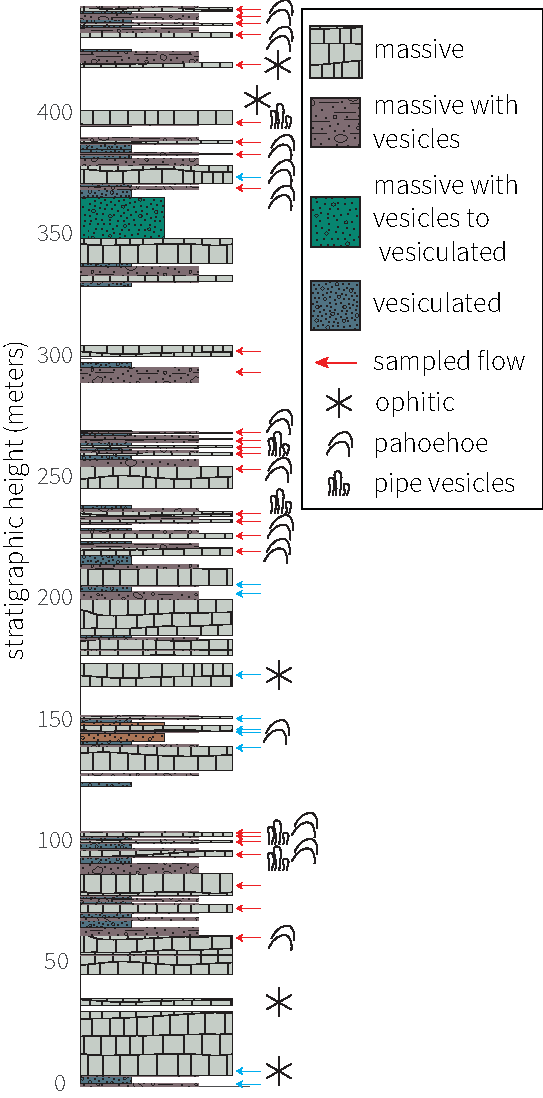
\includegraphics{../data/SLB/plots/SLB_strat.pdf}\\

Additionally, a broader map view of the stack of lava flows highlights the discontinuity of the two VGP populations.\\

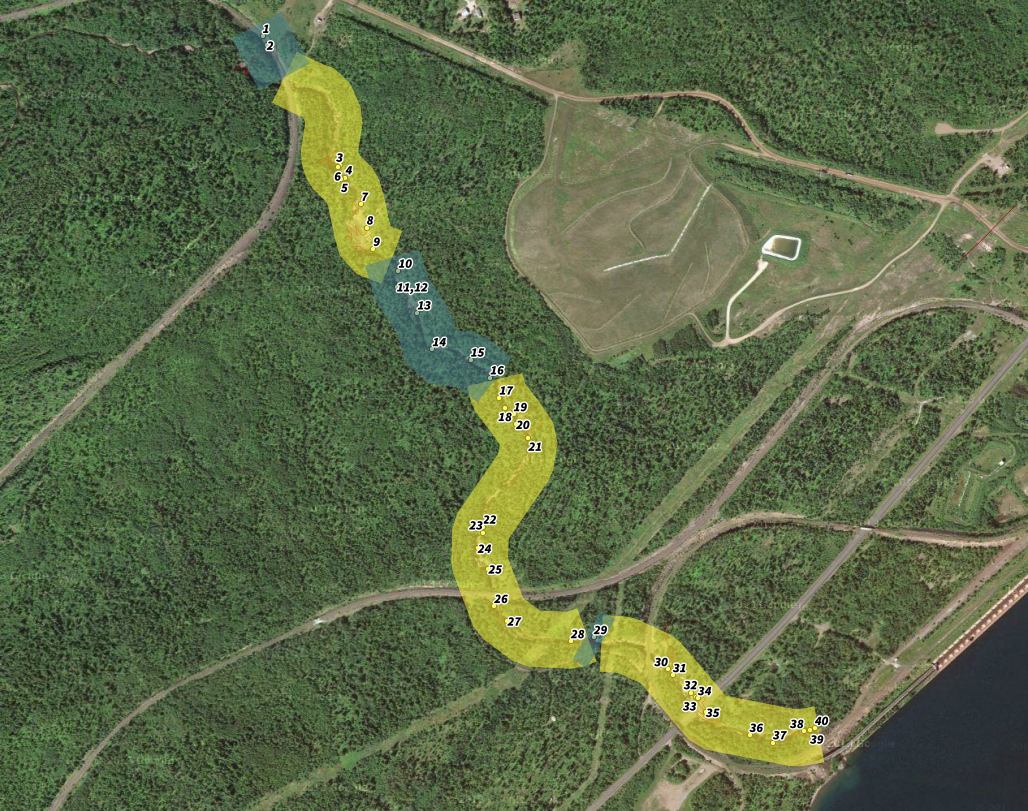
\includegraphics[width=\textwidth]{../data/SLB/plots/SLB_shadedbyVGPlat.png}\\

One last way to approach this problem is to inspect the path of the
paleomagnetic poles being traced out by secular variation. We can look
for potential patterns in the path of the poles through time by
considering each cooling unit's stratigraphic placement.

    \begin{Verbatim}[commandchars=\\\{\}]
{\color{incolor}In [{\color{incolor}21}]:} \PY{c+c1}{\PYZsh{} upload strat heights}
         \PY{n}{SLB\PYZus{}strat\PYZus{}df} \PY{o}{=} \PY{n}{pd}\PY{o}{.}\PY{n}{read\PYZus{}csv}\PY{p}{(}\PY{l+s+s1}{\PYZsq{}}\PY{l+s+s1}{../Data/SLB/er\PYZus{}sites.txt}\PY{l+s+s1}{\PYZsq{}}\PY{p}{,} \PY{n}{sep}\PY{o}{=}\PY{l+s+s1}{\PYZsq{}}\PY{l+s+se}{\PYZbs{}t}\PY{l+s+s1}{\PYZsq{}}\PY{p}{,} \PY{n}{skiprows}\PY{o}{=}\PY{l+m+mi}{1}\PY{p}{,} 
                                    \PY{n}{usecols}\PY{o}{=}\PY{p}{[}\PY{l+s+s1}{\PYZsq{}}\PY{l+s+s1}{er\PYZus{}site\PYZus{}name}\PY{l+s+s1}{\PYZsq{}}\PY{p}{,} \PY{l+s+s1}{\PYZsq{}}\PY{l+s+s1}{site\PYZus{}height}\PY{l+s+s1}{\PYZsq{}}\PY{p}{]}\PY{p}{)}
         \PY{n}{SLB\PYZus{}strat\PYZus{}df} \PY{o}{=} \PY{n}{SLB\PYZus{}strat\PYZus{}df}\PY{o}{.}\PY{n}{set\PYZus{}index}\PY{p}{(}\PY{l+s+s1}{\PYZsq{}}\PY{l+s+s1}{er\PYZus{}site\PYZus{}name}\PY{l+s+s1}{\PYZsq{}}\PY{p}{)}
         
         \PY{n}{m} \PY{o}{=} \PY{n}{pole\PYZus{}figure\PYZus{}appearance}\PY{p}{(}\PY{p}{)}
         
         \PY{n}{centerlon}\PY{p}{,} \PY{n}{centerlat} \PY{o}{=} \PY{n}{m}\PY{p}{(}\PY{n}{SLB\PYZus{}Data}\PY{p}{[}\PY{l+s+s1}{\PYZsq{}}\PY{l+s+s1}{vgp\PYZus{}lon}\PY{l+s+s1}{\PYZsq{}}\PY{p}{]}\PY{o}{.}\PY{n}{tolist}\PY{p}{(}\PY{p}{)}\PY{p}{,}\PY{n}{SLB\PYZus{}Data}\PY{p}{[}\PY{l+s+s1}{\PYZsq{}}\PY{l+s+s1}{vgp\PYZus{}lat}\PY{l+s+s1}{\PYZsq{}}\PY{p}{]}\PY{o}{.}\PY{n}{tolist}\PY{p}{(}\PY{p}{)}\PY{p}{)}
         \PY{n}{m}\PY{o}{.}\PY{n}{plot}\PY{p}{(}\PY{n}{centerlon}\PY{p}{,} \PY{n}{centerlat}\PY{p}{,} \PY{n}{alpha}\PY{o}{=}\PY{l+m+mf}{0.5}\PY{p}{,} \PY{n}{zorder}\PY{o}{=}\PY{l+m+mi}{1}\PY{p}{)}
         \PY{n}{m}\PY{o}{.}\PY{n}{scatter}\PY{p}{(}\PY{n}{centerlon}\PY{p}{,} \PY{n}{centerlat}\PY{p}{,} \PY{n}{marker}\PY{o}{=}\PY{l+s+s1}{\PYZsq{}}\PY{l+s+s1}{.}\PY{l+s+s1}{\PYZsq{}}\PY{p}{,} \PY{n}{s}\PY{o}{=}\PY{l+m+mf}{300.0}\PY{p}{,} 
                  \PY{n}{c} \PY{o}{=} \PY{n}{SLB\PYZus{}strat\PYZus{}df}\PY{o}{.}\PY{n}{site\PYZus{}height}\PY{o}{.}\PY{n}{tolist}\PY{p}{(}\PY{p}{)}\PY{p}{,} \PY{n}{cmap}\PY{o}{=}\PY{l+s+s1}{\PYZsq{}}\PY{l+s+s1}{Paired}\PY{l+s+s1}{\PYZsq{}}\PY{p}{,} \PY{n}{zorder}\PY{o}{=}\PY{l+m+mi}{2}\PY{p}{)}
         
         \PY{n}{plt}\PY{o}{.}\PY{n}{colorbar}\PY{p}{(}\PY{n}{label}\PY{o}{=}\PY{l+s+s1}{\PYZsq{}}\PY{l+s+s1}{Stratigraphy (meters)}\PY{l+s+s1}{\PYZsq{}}\PY{p}{,} \PY{n}{shrink}\PY{o}{=}\PY{l+m+mf}{0.7}\PY{p}{)}
         \PY{n}{plt}\PY{o}{.}\PY{n}{show}\PY{p}{(}\PY{p}{)}
\end{Verbatim}

    \begin{center}
    \adjustimage{max size={0.7\linewidth}{0.7\paperheight}}{Late_Rift_Data_Analysis_files/Late_Rift_Data_Analysis_34_0.pdf}
    \end{center}
    
    From this view, we notice the relatively tight grouping of poles among
certain stratigraphic intervals as they trace out sections of the entire
distribution. However, there is still no apparent explanation for the
occasional excursion of the geomagnetic pole to lower latitudes. It
therefore seems likely that the divergence of these two VGP populations
can be attributed to a recurrent geomagnetic excursional behavior rather than a
post-emplacement offset of magnetizations. We also note the similarity
of this anomalous behavior to the distribution of paleomagnetic poles
from the Lake Shore Traps (see below).

    \subsection{Combine new SLB data with Tauxe and Kodama
(2009)}\label{combine-new-slb-data-with-tauxe-and-kodama-2009}

    \begin{Verbatim}[commandchars=\\\{\}]
{\color{incolor}In [{\color{incolor}22}]:} \PY{n}{combined\PYZus{}SLB\PYZus{}lon} \PY{o}{=} \PY{n}{NSVG\PYZus{}nsl}\PY{p}{[}\PY{l+s+s1}{\PYZsq{}}\PY{l+s+s1}{pole\PYZus{}lon}\PY{l+s+s1}{\PYZsq{}}\PY{p}{]}\PY{o}{.}\PY{n}{tolist}\PY{p}{(}\PY{p}{)} \PY{o}{+} \PY{n}{SLB\PYZus{}Data}\PY{p}{[}\PY{l+s+s1}{\PYZsq{}}\PY{l+s+s1}{vgp\PYZus{}lon}\PY{l+s+s1}{\PYZsq{}}\PY{p}{]}\PY{o}{.}\PY{n}{tolist}\PY{p}{(}\PY{p}{)}
         \PY{n}{combined\PYZus{}SLB\PYZus{}lat} \PY{o}{=} \PY{n}{NSVG\PYZus{}nsl}\PY{p}{[}\PY{l+s+s1}{\PYZsq{}}\PY{l+s+s1}{pole\PYZus{}lat}\PY{l+s+s1}{\PYZsq{}}\PY{p}{]}\PY{o}{.}\PY{n}{tolist}\PY{p}{(}\PY{p}{)} \PY{o}{+} \PY{n}{SLB\PYZus{}Data}\PY{p}{[}\PY{l+s+s1}{\PYZsq{}}\PY{l+s+s1}{vgp\PYZus{}lat}\PY{l+s+s1}{\PYZsq{}}\PY{p}{]}\PY{o}{.}\PY{n}{tolist}\PY{p}{(}\PY{p}{)}
         \PY{n}{combined\PYZus{}SLB\PYZus{}mean} \PY{o}{=} \PY{n}{ipmag}\PY{o}{.}\PY{n}{fisher\PYZus{}mean}\PY{p}{(}\PY{n}{combined\PYZus{}SLB\PYZus{}lon}\PY{p}{,}\PY{n}{combined\PYZus{}SLB\PYZus{}lat}\PY{p}{)}
\end{Verbatim}

    \begin{Verbatim}[commandchars=\\\{\}]
{\color{incolor}In [{\color{incolor}23}]:} \PY{n}{m} \PY{o}{=} \PY{n}{pole\PYZus{}figure\PYZus{}appearance}\PY{p}{(}\PY{p}{)}
         \PY{n}{ipmag}\PY{o}{.}\PY{n}{plot\PYZus{}pole}\PY{p}{(}\PY{n}{m}\PY{p}{,}\PY{n}{NSVG\PYZus{}nswu\PYZus{}mean}\PY{p}{[}\PY{l+s+s1}{\PYZsq{}}\PY{l+s+s1}{dec}\PY{l+s+s1}{\PYZsq{}}\PY{p}{]}\PY{p}{,}\PY{n}{NSVG\PYZus{}nswu\PYZus{}mean}\PY{p}{[}\PY{l+s+s1}{\PYZsq{}}\PY{l+s+s1}{inc}\PY{l+s+s1}{\PYZsq{}}\PY{p}{]}\PY{p}{,}
                         \PY{n}{NSVG\PYZus{}nswu\PYZus{}mean}\PY{p}{[}\PY{l+s+s1}{\PYZsq{}}\PY{l+s+s1}{alpha95}\PY{l+s+s1}{\PYZsq{}}\PY{p}{]}\PY{p}{,} \PY{n}{marker}\PY{o}{=}\PY{l+s+s1}{\PYZsq{}}\PY{l+s+s1}{s}\PY{l+s+s1}{\PYZsq{}}\PY{p}{,}\PY{n}{color}\PY{o}{=}\PY{l+s+s1}{\PYZsq{}}\PY{l+s+s1}{b}\PY{l+s+s1}{\PYZsq{}}\PY{p}{,}
                         \PY{n}{label}\PY{o}{=}\PY{l+s+s1}{\PYZsq{}}\PY{l+s+s1}{NSVG mean (nswu; Tauxe and Kodama (2009))}\PY{l+s+s1}{\PYZsq{}}\PY{p}{)}
         \PY{n}{ipmag}\PY{o}{.}\PY{n}{plot\PYZus{}vgp}\PY{p}{(}\PY{n}{m}\PY{p}{,}\PY{n}{combined\PYZus{}SLB\PYZus{}lon}\PY{p}{,}\PY{n}{combined\PYZus{}SLB\PYZus{}lat}\PY{p}{,} \PY{n}{color}\PY{o}{=}\PY{l+s+s1}{\PYZsq{}}\PY{l+s+s1}{g}\PY{l+s+s1}{\PYZsq{}}\PY{p}{,}
                        \PY{n}{label}\PY{o}{=}\PY{l+s+s1}{\PYZsq{}}\PY{l+s+s1}{combined SLB (this study and Tauxe and Kodama (2009))}\PY{l+s+s1}{\PYZsq{}}\PY{p}{)}
         \PY{n}{ipmag}\PY{o}{.}\PY{n}{plot\PYZus{}vgp}\PY{p}{(}\PY{n}{m}\PY{p}{,}\PY{n}{NSVG\PYZus{}nsl}\PY{p}{[}\PY{l+s+s1}{\PYZsq{}}\PY{l+s+s1}{pole\PYZus{}lon}\PY{l+s+s1}{\PYZsq{}}\PY{p}{]}\PY{o}{.}\PY{n}{tolist}\PY{p}{(}\PY{p}{)}\PY{p}{,}\PY{n}{NSVG\PYZus{}nsl}\PY{p}{[}\PY{l+s+s1}{\PYZsq{}}\PY{l+s+s1}{pole\PYZus{}lat}\PY{l+s+s1}{\PYZsq{}}\PY{p}{]}\PY{o}{.}\PY{n}{tolist}\PY{p}{(}\PY{p}{)}\PY{p}{,}
                        \PY{n}{color}\PY{o}{=}\PY{l+s+s1}{\PYZsq{}}\PY{l+s+s1}{springgreen}\PY{l+s+s1}{\PYZsq{}}\PY{p}{,}\PY{n}{label}\PY{o}{=}\PY{l+s+s1}{\PYZsq{}}\PY{l+s+s1}{SLB (nsl; Tauxe and Kodama (2009))}\PY{l+s+s1}{\PYZsq{}}\PY{p}{)}
         \PY{n}{ipmag}\PY{o}{.}\PY{n}{plot\PYZus{}pole}\PY{p}{(}\PY{n}{m}\PY{p}{,}\PY{n}{combined\PYZus{}SLB\PYZus{}mean}\PY{p}{[}\PY{l+s+s1}{\PYZsq{}}\PY{l+s+s1}{dec}\PY{l+s+s1}{\PYZsq{}}\PY{p}{]}\PY{p}{,}\PY{n}{combined\PYZus{}SLB\PYZus{}mean}\PY{p}{[}\PY{l+s+s1}{\PYZsq{}}\PY{l+s+s1}{inc}\PY{l+s+s1}{\PYZsq{}}\PY{p}{]}\PY{p}{,}
                         \PY{n}{combined\PYZus{}SLB\PYZus{}mean}\PY{p}{[}\PY{l+s+s1}{\PYZsq{}}\PY{l+s+s1}{alpha95}\PY{l+s+s1}{\PYZsq{}}\PY{p}{]}\PY{p}{,} \PY{n}{marker}\PY{o}{=}\PY{l+s+s1}{\PYZsq{}}\PY{l+s+s1}{s}\PY{l+s+s1}{\PYZsq{}}\PY{p}{,}\PY{n}{color}\PY{o}{=}\PY{l+s+s1}{\PYZsq{}}\PY{l+s+s1}{g}\PY{l+s+s1}{\PYZsq{}}\PY{p}{)}
         
         \PY{n}{ipmag}\PY{o}{.}\PY{n}{print\PYZus{}pole\PYZus{}mean}\PY{p}{(}\PY{n}{combined\PYZus{}SLB\PYZus{}mean}\PY{p}{)}
         
         \PY{n}{plt}\PY{o}{.}\PY{n}{legend}\PY{p}{(}\PY{p}{)}
         \PY{n}{plt}\PY{o}{.}\PY{n}{savefig}\PY{p}{(}\PY{l+s+s1}{\PYZsq{}}\PY{l+s+s1}{./Code\PYZus{}output/NSVG\PYZus{}SLB\PYZus{}poles\PYZus{}combined.pdf}\PY{l+s+s1}{\PYZsq{}}\PY{p}{)}
         \PY{n}{plt}\PY{o}{.}\PY{n}{show}\PY{p}{(}\PY{p}{)}
\end{Verbatim}

    \begin{Verbatim}[commandchars=\\\{\}]
Plong: 187.8  Plat: 27.1
Number of directions in mean (n): 50
Angular radius of 95\% confidence (A\_95): 3.0
Precision parameter (k) estimate: 46.5
    \end{Verbatim}

    \begin{center}
    \adjustimage{max size={0.6\linewidth}{0.6\paperheight}}{Late_Rift_Data_Analysis_files/Late_Rift_Data_Analysis_38_1.pdf}
    \end{center}
    
This combined VGPs are non-Fisherian in distribution as seen in the Fisher Q--Q test below.
    
    \begin{Verbatim}[commandchars=\\\{\}]
{\color{incolor}In [{\color{incolor}24}]:} \PY{n}{ipmag}\PY{o}{.}\PY{n}{fishqq}\PY{p}{(}\PY{n}{combined\PYZus{}SLB\PYZus{}lon}\PY{p}{,}\PY{n}{combined\PYZus{}SLB\PYZus{}lat}\PY{p}{)}
\end{Verbatim}

            \begin{Verbatim}[commandchars=\\\{\}]
{\color{outcolor}Out[{\color{outcolor}24}]:} \{'Dec': 187.79191234206988,
          'Inc': 27.199685356762615,
          'Me': 0.53556909069644332,
          'Me\_critical': 1.094,
          'Mode': 'Mode 1',
          'Mu': 1.4805683534761531,
          'Mu\_critical': 1.207,
          'N': 50,
          'Test\_result': 'Fisherian model rejected'\}
\end{Verbatim}
        
    \begin{center}
    \adjustimage{max size={0.9\linewidth}{0.9\paperheight}}{Late_Rift_Data_Analysis_files/Late_Rift_Data_Analysis_42_1.pdf}
    \end{center}
%    { \hspace*{\fill} \\}
%    
%    \begin{center}
%    \adjustimage{max size={0.9\linewidth}{0.9\paperheight}}{Late_Rift_Data_Analysis_files/Late_Rift_Data_Analysis_39_2.pdf}
%    \end{center}
%    { \hspace*{\fill} \\}
    
\section{Lake Shore Traps}\label{lake-shore-traps}

We first import paleomagnetic from \cite{Diehl1994a}. 

    \begin{Verbatim}[commandchars=\\\{\}]
{\color{incolor}In [{\color{incolor}25}]:} \PY{n}{Diehl1994a\PYZus{}LST\PYZus{}Data\PYZus{}all}\PY{o}{=}\PY{n}{pd}\PY{o}{.}\PY{n}{read\PYZus{}csv}\PY{p}{(}\PY{l+s+s1}{\PYZsq{}}\PY{l+s+s1}{../Data/Previous\PYZus{}studies/Diehl1994a\PYZus{}data.csv}\PY{l+s+s1}{\PYZsq{}}\PY{p}{,}\PY{n}{sep}\PY{o}{=}\PY{l+s+s1}{\PYZsq{}}\PY{l+s+s1}{,}\PY{l+s+s1}{\PYZsq{}}\PY{p}{)}
         \PY{c+c1}{\PYZsh{}Kulakov2013 reported data for the flow LST28 that supersedes }
         \PY{c+c1}{\PYZsh{}the Diehl direction which should accordingly be dropped}
         \PY{n}{Diehl1994a\PYZus{}LST\PYZus{}Data}\PY{o}{=}\PY{n}{Diehl1994a\PYZus{}LST\PYZus{}Data\PYZus{}all}\PY{o}{.}\PY{n}{drop}\PY{p}{(}\PY{l+m+mi}{17}\PY{p}{)}
         \PY{n}{Diehl1994a\PYZus{}LST\PYZus{}Data}\PY{o}{.}\PY{n}{reset\PYZus{}index}\PY{p}{(}\PY{n}{inplace}\PY{o}{=}\PY{n+nb+bp}{True}\PY{p}{)}
         \PY{n}{Diehl1994a\PYZus{}LST\PYZus{}Data}\PY{o}{.}\PY{n}{head}\PY{p}{(}\PY{p}{)}
\end{Verbatim}

%            \begin{Verbatim}[commandchars=\\\{\}]
%See Data Repository file under \texttt{/Data/Previous\_studies/Diehl1994a.csv} to view the data of Diehl and Haig (1994)
%\end{Verbatim}
\noindent This file can be found in the Data Repository under \texttt{/Data/Previous\_studies/Diehl1994a\_data.csv}.\\ 

\noindent Next, we import paleomagnetic data from \cite{Kulakov2013a}. The original \cite{Kulakov2013a} data set incorporated the data of \cite{Diehl1994a}; however, we elect to manually combine these data and recalculate the associated grand mean here.
        
    \begin{Verbatim}[commandchars=\\\{\}]
{\color{incolor}In [{\color{incolor}26}]:} \PY{n}{Kulakov2013a\PYZus{}LST\PYZus{}Data}\PY{o}{=}\PY{n}{pd}\PY{o}{.}\PY{n}{read\PYZus{}csv}\PY{p}{(}\PY{l+s+s1}{\PYZsq{}}\PY{l+s+s1}{../Data/Previous\PYZus{}studies/Kulakov2013a\PYZus{}data.csv}\PY{l+s+s1}{\PYZsq{}}\PY{p}{,}\PY{n}{sep}\PY{o}{=}\PY{l+s+s1}{\PYZsq{}}\PY{l+s+s1}{,}\PY{l+s+s1}{\PYZsq{}}\PY{p}{)}
         \PY{n}{Kulakov2013a\PYZus{}LST\PYZus{}Data}\PY{o}{.}\PY{n}{head}\PY{p}{(}\PY{p}{)}
\end{Verbatim}

%            \begin{Verbatim}[commandchars=\\\{\}]
%{\color{outcolor}Out[{\color{outcolor}26}]:} \href{run:../Data/Previous_studies/Kulakov2013a_data.csv}{Click to view the data of Kulakov et al. (2013)}
%\end{Verbatim}
\noindent This file can be found in the Data Repository under \texttt{/Data/Previous\_studies/Kulakov2013a\_data.csv}.\\ 

        
    \begin{Verbatim}[commandchars=\\\{\}]
{\color{incolor}In [{\color{incolor}27}]:} \PY{n}{LST\PYZus{}Diehl\PYZus{}VGPs}\PY{o}{=}\PY{n}{ipmag}\PY{o}{.}\PY{n}{make\PYZus{}di\PYZus{}block}\PY{p}{(}\PY{n}{Diehl1994a\PYZus{}LST\PYZus{}Data}\PY{p}{[}\PY{l+s+s1}{\PYZsq{}}\PY{l+s+s1}{vgp\PYZus{}lon}\PY{l+s+s1}{\PYZsq{}}\PY{p}{]}\PY{p}{,}
                                            \PY{n}{Diehl1994a\PYZus{}LST\PYZus{}Data}\PY{p}{[}\PY{l+s+s1}{\PYZsq{}}\PY{l+s+s1}{vgp\PYZus{}lat}\PY{l+s+s1}{\PYZsq{}}\PY{p}{]}\PY{p}{)}
         
         \PY{n}{LST\PYZus{}Kulakov\PYZus{}VGPs}\PY{o}{=}\PY{n}{ipmag}\PY{o}{.}\PY{n}{make\PYZus{}di\PYZus{}block}\PY{p}{(}\PY{n}{Kulakov2013a\PYZus{}LST\PYZus{}Data}\PY{p}{[}\PY{l+s+s1}{\PYZsq{}}\PY{l+s+s1}{vgp\PYZus{}lon}\PY{l+s+s1}{\PYZsq{}}\PY{p}{]}\PY{p}{,}
                                              \PY{n}{Kulakov2013a\PYZus{}LST\PYZus{}Data}\PY{p}{[}\PY{l+s+s1}{\PYZsq{}}\PY{l+s+s1}{vgp\PYZus{}lat}\PY{l+s+s1}{\PYZsq{}}\PY{p}{]}\PY{p}{)}
         
         \PY{n}{LST\PYZus{}VGPs}\PY{o}{=}\PY{n}{np}\PY{o}{.}\PY{n}{concatenate}\PY{p}{(}\PY{p}{(}\PY{n}{LST\PYZus{}Diehl\PYZus{}VGPs}\PY{p}{,}\PY{n}{LST\PYZus{}Kulakov\PYZus{}VGPs}\PY{p}{)}\PY{p}{)}
         
         \PY{n}{LST\PYZus{}Diehl\PYZus{}mean} \PY{o}{=} \PY{n}{pmag}\PY{o}{.}\PY{n}{fisher\PYZus{}mean}\PY{p}{(}\PY{n}{LST\PYZus{}Diehl\PYZus{}VGPs}\PY{p}{)}
         \PY{n}{LST\PYZus{}Kulakov\PYZus{}mean}\PY{o}{=}\PY{n}{pmag}\PY{o}{.}\PY{n}{fisher\PYZus{}mean}\PY{p}{(}\PY{n}{LST\PYZus{}Kulakov\PYZus{}VGPs}\PY{p}{)}
         \PY{n}{LST\PYZus{}all\PYZus{}mean}\PY{o}{=}\PY{n}{pmag}\PY{o}{.}\PY{n}{fisher\PYZus{}mean}\PY{p}{(}\PY{n}{LST\PYZus{}VGPs}\PY{p}{)}
\end{Verbatim}

    \begin{Verbatim}[commandchars=\\\{\}]
{\color{incolor}In [{\color{incolor}28}]:} \PY{n}{m} \PY{o}{=} \PY{n}{Basemap}\PY{p}{(}\PY{n}{projection}\PY{o}{=}\PY{l+s+s1}{\PYZsq{}}\PY{l+s+s1}{ortho}\PY{l+s+s1}{\PYZsq{}}\PY{p}{,}\PY{n}{lat\PYZus{}0}\PY{o}{=}\PY{l+m+mi}{35}\PY{p}{,}\PY{n}{lon\PYZus{}0}\PY{o}{=}\PY{l+m+mi}{200}\PY{p}{,}\PY{n}{resolution}\PY{o}{=}\PY{l+s+s1}{\PYZsq{}}\PY{l+s+s1}{c}\PY{l+s+s1}{\PYZsq{}}\PY{p}{,}
                     \PY{n}{area\PYZus{}thresh}\PY{o}{=}\PY{l+m+mi}{50000}\PY{p}{)}
         \PY{n}{pole\PYZus{}figure\PYZus{}appearance}\PY{p}{(}\PY{p}{)}
         
         \PY{n}{ipmag}\PY{o}{.}\PY{n}{plot\PYZus{}vgp}\PY{p}{(}\PY{n}{m}\PY{p}{,}\PY{n}{Diehl1994a\PYZus{}LST\PYZus{}Data}\PY{p}{[}\PY{l+s+s1}{\PYZsq{}}\PY{l+s+s1}{vgp\PYZus{}lon}\PY{l+s+s1}{\PYZsq{}}\PY{p}{]}\PY{o}{.}\PY{n}{tolist}\PY{p}{(}\PY{p}{)}\PY{p}{,}
                        \PY{n}{Diehl1994a\PYZus{}LST\PYZus{}Data}\PY{p}{[}\PY{l+s+s1}{\PYZsq{}}\PY{l+s+s1}{vgp\PYZus{}lat}\PY{l+s+s1}{\PYZsq{}}\PY{p}{]}\PY{o}{.}\PY{n}{tolist}\PY{p}{(}\PY{p}{)}\PY{p}{,}
                       \PY{n}{label}\PY{o}{=}\PY{l+s+s1}{\PYZsq{}}\PY{l+s+s1}{LST dikes VGPs (Diehl1994a)}\PY{l+s+s1}{\PYZsq{}}\PY{p}{,}\PY{n}{color}\PY{o}{=}\PY{l+s+s1}{\PYZsq{}}\PY{l+s+s1}{r}\PY{l+s+s1}{\PYZsq{}}\PY{p}{)}
         \PY{n}{ipmag}\PY{o}{.}\PY{n}{plot\PYZus{}vgp}\PY{p}{(}\PY{n}{m}\PY{p}{,}\PY{n}{Kulakov2013a\PYZus{}LST\PYZus{}Data}\PY{p}{[}\PY{l+s+s1}{\PYZsq{}}\PY{l+s+s1}{vgp\PYZus{}lon}\PY{l+s+s1}{\PYZsq{}}\PY{p}{]}\PY{o}{.}\PY{n}{tolist}\PY{p}{(}\PY{p}{)}\PY{p}{,}
                        \PY{n}{Kulakov2013a\PYZus{}LST\PYZus{}Data}\PY{p}{[}\PY{l+s+s1}{\PYZsq{}}\PY{l+s+s1}{vgp\PYZus{}lat}\PY{l+s+s1}{\PYZsq{}}\PY{p}{]}\PY{o}{.}\PY{n}{tolist}\PY{p}{(}\PY{p}{)}\PY{p}{,}
                       \PY{n}{label}\PY{o}{=}\PY{l+s+s1}{\PYZsq{}}\PY{l+s+s1}{LST dikes VGPs (Kulakov2013a)}\PY{l+s+s1}{\PYZsq{}}\PY{p}{,}\PY{n}{color}\PY{o}{=}\PY{l+s+s1}{\PYZsq{}}\PY{l+s+s1}{b}\PY{l+s+s1}{\PYZsq{}}\PY{p}{)}
         \PY{n}{ipmag}\PY{o}{.}\PY{n}{plot\PYZus{}pole}\PY{p}{(}\PY{n}{m}\PY{p}{,}\PY{n}{LST\PYZus{}all\PYZus{}mean}\PY{p}{[}\PY{l+s+s1}{\PYZsq{}}\PY{l+s+s1}{dec}\PY{l+s+s1}{\PYZsq{}}\PY{p}{]}\PY{p}{,}\PY{n}{LST\PYZus{}all\PYZus{}mean}\PY{p}{[}\PY{l+s+s1}{\PYZsq{}}\PY{l+s+s1}{inc}\PY{l+s+s1}{\PYZsq{}}\PY{p}{]}\PY{p}{,}
                         \PY{n}{LST\PYZus{}all\PYZus{}mean}\PY{p}{[}\PY{l+s+s1}{\PYZsq{}}\PY{l+s+s1}{alpha95}\PY{l+s+s1}{\PYZsq{}}\PY{p}{]}\PY{p}{,} \PY{n}{label}\PY{o}{=}\PY{l+s+s1}{\PYZsq{}}\PY{l+s+s1}{LST dikes mean pole}\PY{l+s+s1}{\PYZsq{}}\PY{p}{,}\PY{n}{marker}\PY{o}{=}\PY{l+s+s1}{\PYZsq{}}\PY{l+s+s1}{s}\PY{l+s+s1}{\PYZsq{}}\PY{p}{)}
         \PY{n}{ipmag}\PY{o}{.}\PY{n}{plot\PYZus{}pole}\PY{p}{(}\PY{n}{m}\PY{p}{,}\PY{n}{LST\PYZus{}Diehl\PYZus{}mean}\PY{p}{[}\PY{l+s+s1}{\PYZsq{}}\PY{l+s+s1}{dec}\PY{l+s+s1}{\PYZsq{}}\PY{p}{]}\PY{p}{,}\PY{n}{LST\PYZus{}Diehl\PYZus{}mean}\PY{p}{[}\PY{l+s+s1}{\PYZsq{}}\PY{l+s+s1}{inc}\PY{l+s+s1}{\PYZsq{}}\PY{p}{]}\PY{p}{,}
                         \PY{n}{LST\PYZus{}Diehl\PYZus{}mean}\PY{p}{[}\PY{l+s+s1}{\PYZsq{}}\PY{l+s+s1}{alpha95}\PY{l+s+s1}{\PYZsq{}}\PY{p}{]}\PY{p}{,} \PY{n}{color}\PY{o}{=}\PY{l+s+s1}{\PYZsq{}}\PY{l+s+s1}{r}\PY{l+s+s1}{\PYZsq{}}\PY{p}{,}
                         \PY{n}{label}\PY{o}{=}\PY{l+s+s1}{\PYZsq{}}\PY{l+s+s1}{Diehl1994a mean}\PY{l+s+s1}{\PYZsq{}}\PY{p}{,}\PY{n}{marker}\PY{o}{=}\PY{l+s+s1}{\PYZsq{}}\PY{l+s+s1}{s}\PY{l+s+s1}{\PYZsq{}}\PY{p}{)}
         \PY{c+c1}{\PYZsh{}from Kulakov2013a}
         \PY{n}{ipmag}\PY{o}{.}\PY{n}{plot\PYZus{}pole}\PY{p}{(}\PY{n}{m}\PY{p}{,}\PY{l+m+mf}{186.4}\PY{p}{,}\PY{l+m+mf}{23.1}\PY{p}{,}\PY{l+m+mf}{4.0}\PY{p}{,}\PY{n}{color}\PY{o}{=}\PY{l+s+s1}{\PYZsq{}}\PY{l+s+s1}{g}\PY{l+s+s1}{\PYZsq{}}\PY{p}{,}
                         \PY{n}{label}\PY{o}{=}\PY{l+s+s1}{\PYZsq{}}\PY{l+s+s1}{mean as calculated in Kulakov2013a}\PY{l+s+s1}{\PYZsq{}}\PY{p}{,}\PY{n}{marker}\PY{o}{=}\PY{l+s+s1}{\PYZsq{}}\PY{l+s+s1}{s}\PY{l+s+s1}{\PYZsq{}}\PY{p}{)}
         
         \PY{n}{plt}\PY{o}{.}\PY{n}{legend}\PY{p}{(}\PY{n}{loc}\PY{o}{=}\PY{l+m+mi}{4}\PY{p}{)}
         \PY{n}{plt}\PY{o}{.}\PY{n}{savefig}\PY{p}{(}\PY{l+s+s1}{\PYZsq{}}\PY{l+s+s1}{Code\PYZus{}output/LST\PYZus{}vgps.pdf}\PY{l+s+s1}{\PYZsq{}}\PY{p}{)}
         \PY{n}{plt}\PY{o}{.}\PY{n}{show}\PY{p}{(}\PY{p}{)}
\end{Verbatim}

    \begin{center}
    \adjustimage{max size={0.6\linewidth}{0.6\paperheight}}{Late_Rift_Data_Analysis_files/Late_Rift_Data_Analysis_44_0.pdf}
    \end{center}
    
    Here we test whether the distribution of Lake Shore Traps VGPs are
Fisherian.

    \begin{Verbatim}[commandchars=\\\{\}]
{\color{incolor}In [{\color{incolor}29}]:} \PY{n}{ipmag}\PY{o}{.}\PY{n}{fishqq}\PY{p}{(}\PY{n}{di\PYZus{}block}\PY{o}{=}\PY{n}{LST\PYZus{}VGPs}\PY{p}{)}
\end{Verbatim}

            \begin{Verbatim}[commandchars=\\\{\}]
{\color{outcolor}Out[{\color{outcolor}29}]:} \{'Dec': 185.61848690207148,
          'Inc': 23.207239038463833,
          'Me': 1.1080580586218494,
          'Me\_critical': 1.094,
          'Mode': 'Mode 1',
          'Mu': 1.8795789739707827,
          'Mu\_critical': 1.207,
          'N': 49,
          'Test\_result': 'Fisherian model rejected'\}
\end{Verbatim}
        
    \begin{center}
    \adjustimage{max size={0.9\linewidth}{0.9\paperheight}}{Late_Rift_Data_Analysis_files/Late_Rift_Data_Analysis_49_1.pdf}
    \end{center}
%    { \hspace*{\fill} \\}
%    
%    \begin{center}
%    \adjustimage{max size={0.9\linewidth}{0.9\paperheight}}{Late_Rift_Data_Analysis_files/Late_Rift_Data_Analysis_46_2.pdf}
%    \end{center}
%    { \hspace*{\fill} \\}

Here we test for a common mean between the Lake Shore Traps VGPs and our newly combined data from the Schroeder-Lutsen basalts.
    \begin{Verbatim}[commandchars=\\\{\}]
{\color{incolor}In [{\color{incolor}30}]:} \PY{n}{ipmag}\PY{o}{.}\PY{n}{common\PYZus{}mean\PYZus{}bootstrap}\PY{p}{(}\PY{n}{LST\PYZus{}VGPs}\PY{p}{,}\PY{n}{ipmag}\PY{o}{.}\PY{n}{make\PYZus{}di\PYZus{}block}\PY{p}{(}\PY{n}{combined\PYZus{}SLB\PYZus{}lon}\PY{p}{,}
                                                                  \PY{n}{combined\PYZus{}SLB\PYZus{}lat}\PY{p}{)}\PY{p}{)}
\end{Verbatim}

    \begin{center}
    \adjustimage{max size={0.9\linewidth}{0.9\paperheight}}{Late_Rift_Data_Analysis_files/Late_Rift_Data_Analysis_47_0.pdf}
    \end{center}
    
    \begin{Verbatim}[commandchars=\\\{\}]
{\color{incolor}In [{\color{incolor}31}]:} \PY{n}{ipmag}\PY{o}{.}\PY{n}{common\PYZus{}mean\PYZus{}watson}\PY{p}{(}\PY{n}{LST\PYZus{}VGPs}\PY{p}{,}
                                  \PY{n}{ipmag}\PY{o}{.}\PY{n}{make\PYZus{}di\PYZus{}block}\PY{p}{(}\PY{n}{combined\PYZus{}SLB\PYZus{}lon}\PY{p}{,}\PY{n}{combined\PYZus{}SLB\PYZus{}lat}\PY{p}{)}\PY{p}{,} 
                                  \PY{n}{plot}\PY{o}{=}\PY{l+s+s1}{\PYZsq{}}\PY{l+s+s1}{yes}\PY{l+s+s1}{\PYZsq{}}\PY{p}{)}
\end{Verbatim}

    \begin{Verbatim}[commandchars=\\\{\}]
Results of Watson V test: 

Watson's V:           6.0
Critical value of V:  5.9
"Fail": Since V is greater than Vcrit, the two means can
be distinguished at the 95\% confidence level.

M\&M1990 classification:

Angle between data set means: 4.4
Critical angle for M\&M1990:   4.4
    \end{Verbatim}

    \begin{center}
    \adjustimage{max size={0.9\linewidth}{0.9\paperheight}}{Late_Rift_Data_Analysis_files/Late_Rift_Data_Analysis_48_1.pdf}
    \end{center}
    
\section{Michipicoten Island}\label{michipicoten-island}

\subsection{Palmer and Davis (1987)
data}\label{palmer-and-davis-1987-data}

    \begin{Verbatim}[commandchars=\\\{\}]
{\color{incolor}In [{\color{incolor}32}]:} \PY{n}{Palmer1987\PYZus{}data}\PY{o}{=}\PY{n}{pd}\PY{o}{.}\PY{n}{read\PYZus{}csv}\PY{p}{(}\PY{l+s+s1}{\PYZsq{}}\PY{l+s+s1}{\small{../Data/Previous\PYZus{}studies/Palmer1987a\PYZus{}data\PYZus{}combined\PYZus{}sites.csv}\PY{l+s+s1}{\PYZsq{}}\PY{p}{)}}
         \PY{n}{ipmag}\PY{o}{.}\PY{n}{vgp\PYZus{}calc}\PY{p}{(}\PY{n}{Palmer1987\PYZus{}data}\PY{p}{)}
\end{Verbatim}

\begin{Verbatim}[commandchars=\\\{\}]
{\color{outcolor}Out[{\color{outcolor}32}]:} \href{http://earthref.org/magic/m006169dt20061219133107}{View data of Palmer and Davis (1987) in the MagIC database}
        (http://earthref.org/magic/m006169dt20061219133107)
\end{Verbatim}
\noindent \textbf{NOTE: }If you are having trouble opening the above link to the MagIC database, the file can also be found in the Github repository under \texttt{/Data/Previous\_studies/Palmer1987a\_data\_combined\_sites.csv}.\\  

%\noindent If you are having trouble opening the local file via this link, the file can be found in the Data Repository under \texttt{/Data/Previous\_studies/Palmer1987a\_data\_combined\_sites.csv} and opened manually.\\ 


    The code below splits this dataframe into sites from older main stage
basalts that have been correlated to the Mamainse Point Formation, sites
from the instrusive suite, and sites from the Michipicoten Island
Formation.

While not explicitly described as such, it appears that each of the
sites sampled in \cite{Palmer1987a} are treated as single cooling
units except for site `KM' which is decribed as being collected over a
stratigraphic interval containing multiple flows. As the site is not
from a single cooling unit, data from this are excluded. Also, site 18
is described as coming from a fault bound block with anomalous steep dip
where a structural attitude could not be determined and should be
excluded.

\cite{Palmer1987a} sampled the Channel Lake Member, the Cuesta
Member, and the Davieaux Island Member at multiple sites from which VGPs
were found and used in the final calculation of the Michipicoten Island
Formation mean paleomagnetic pole. However, field observations reveal
that some of these sites represented the redundant sampling of a single
cooling unit, meaning that several VGPs that were originally treated as
independent should have been combined with one another in the final
calculation. Here we reduce the \cite{Palmer1987a} data set to
satisfy these concerns. The reduced number of sites for each
Michipicoten Island Formation member is shown below.

    \begin{Verbatim}[commandchars=\\\{\}]
{\color{incolor}In [{\color{incolor}33}]:} \PY{k}{print} \PY{l+s+s1}{\PYZsq{}}\PY{l+s+s1}{Number of Cuesta Member flows: }\PY{l+s+s1}{\PYZsq{}}\PY{p}{,} 
         \PY{n+nb}{len}\PY{p}{(}\PY{n}{Palmer1987\PYZus{}data}\PY{o}{.}\PY{n}{loc}\PY{p}{[}\PY{n}{Palmer1987\PYZus{}data}\PY{p}{[}\PY{l+s+s1}{\PYZsq{}}\PY{l+s+s1}{member}\PY{l+s+s1}{\PYZsq{}}\PY{p}{]}\PY{o}{==}\PY{l+s+s1}{\PYZsq{}}\PY{l+s+s1}{Cuesta\PYZus{}Member}\PY{l+s+s1}{\PYZsq{}}\PY{p}{]}\PY{p}{)}
         \PY{k}{print} \PY{l+s+s1}{\PYZsq{}}\PY{l+s+s1}{Number of Channel Lake Member flows: }\PY{l+s+s1}{\PYZsq{}}\PY{p}{,}
         \PY{n+nb}{len}\PY{p}{(}\PY{n}{Palmer1987\PYZus{}data}\PY{o}{.}\PY{n}{loc}\PY{p}{[}\PY{n}{Palmer1987\PYZus{}data}\PY{p}{[}\PY{l+s+s1}{\PYZsq{}}\PY{l+s+s1}{member}\PY{l+s+s1}{\PYZsq{}}\PY{p}{]}\PY{o}{==}\PY{l+s+s1}{\PYZsq{}}\PY{l+s+s1}{Channel\PYZus{}Lake\PYZus{}Member}\PY{l+s+s1}{\PYZsq{}}\PY{p}{]}\PY{p}{)}
         \PY{k}{print} \PY{l+s+s1}{\PYZsq{}}\PY{l+s+s1}{Number of Quebec Harbour Member flows: }\PY{l+s+s1}{\PYZsq{}}\PY{p}{,}
         \PY{n+nb}{len}\PY{p}{(}\PY{n}{Palmer1987\PYZus{}data}\PY{o}{.}\PY{n}{loc}\PY{p}{[}\PY{n}{Palmer1987\PYZus{}data}\PY{p}{[}\PY{l+s+s1}{\PYZsq{}}\PY{l+s+s1}{member}\PY{l+s+s1}{\PYZsq{}}\PY{p}{]}\PY{o}{==}\PY{l+s+s1}{\PYZsq{}}\PY{l+s+s1}{Quebec\PYZus{}Harbour\PYZus{}Member}\PY{l+s+s1}{\PYZsq{}}\PY{p}{]}\PY{p}{)}
         \PY{k}{print} \PY{l+s+s1}{\PYZsq{}}\PY{l+s+s1}{Number of South Shore Member flows: }\PY{l+s+s1}{\PYZsq{}}\PY{p}{,}
         \PY{n+nb}{len}\PY{p}{(}\PY{n}{Palmer1987\PYZus{}data}\PY{o}{.}\PY{n}{loc}\PY{p}{[}\PY{n}{Palmer1987\PYZus{}data}\PY{p}{[}\PY{l+s+s1}{\PYZsq{}}\PY{l+s+s1}{member}\PY{l+s+s1}{\PYZsq{}}\PY{p}{]}\PY{o}{==}\PY{l+s+s1}{\PYZsq{}}\PY{l+s+s1}{South\PYZus{}Shore\PYZus{}Member}\PY{l+s+s1}{\PYZsq{}}\PY{p}{]}\PY{p}{)}
         \PY{k}{print} \PY{l+s+s1}{\PYZsq{}}\PY{l+s+s1}{Number of Davieaux Island Member flows: }\PY{l+s+s1}{\PYZsq{}}\PY{p}{,} 
         \PY{n+nb}{len}\PY{p}{(}\PY{n}{Palmer1987\PYZus{}data}\PY{o}{.}\PY{n}{loc}\PY{p}{[}\PY{n}{Palmer1987\PYZus{}data}\PY{p}{[}\PY{l+s+s1}{\PYZsq{}}\PY{l+s+s1}{member}\PY{l+s+s1}{\PYZsq{}}\PY{p}{]}\PY{o}{==}\PY{l+s+s1}{\PYZsq{}}\PY{l+s+s1}{Davieaux\PYZus{}Island\PYZus{}Member}\PY{l+s+s1}{\PYZsq{}}\PY{p}{]}\PY{p}{)}
         \PY{k}{print} \PY{l+s+s1}{\PYZsq{}}\PY{l+s+s1}{Total number of cooling units from the Michipicoten Island Formation: }\PY{l+s+s1}{\PYZsq{}}\PY{p}{,}
         \PY{n+nb}{len}\PY{p}{(}\PY{n}{Palmer1987\PYZus{}data}\PY{o}{.}\PY{n}{loc}\PY{p}{[}\PY{n}{Palmer1987\PYZus{}data}\PY{p}{[}\PY{l+s+s1}{\PYZsq{}}\PY{l+s+s1}{formation}\PY{l+s+s1}{\PYZsq{}}\PY{p}{]}\PY{o}{==}\PY{l+s+s1}{\PYZsq{}}\PY{l+s+s1}{Michipicoten\PYZus{}Island}\PY{l+s+s1}{\PYZsq{}}\PY{p}{]}\PY{p}{)}
\end{Verbatim}

    \begin{Verbatim}[commandchars=\\\{\}]
Number of Cuesta Member flows:  2
Number of Channel Lake Member flows:  1
Number of Quebec Harbour Member flows:  1
Number of South Shore Member flows:  3
Number of Davieaux Island Member flows:  1
Total number of cooling units from the Michipicoten Island Formation:  8
    \end{Verbatim}

    \begin{Verbatim}[commandchars=\\\{\}]
{\color{incolor}In [{\color{incolor}34}]:} \PY{n}{MI\PYZus{}Mamainse\PYZus{}Fm}\PY{o}{=}\PY{n}{Palmer1987\PYZus{}data}\PY{o}{.}\PY{n}{ix}\PY{p}{[}\PY{n}{Palmer1987\PYZus{}data}\PY{p}{[}\PY{l+s+s1}{\PYZsq{}}\PY{l+s+s1}{formation}\PY{l+s+s1}{\PYZsq{}}\PY{p}{]} \PY{o}{==} \PY{l+s+s1}{\PYZsq{}}\PY{l+s+s1}{Quebec\PYZus{}Mine}\PY{l+s+s1}{\PYZsq{}}\PY{p}{]}
         \PY{n}{MI\PYZus{}Mamainse\PYZus{}Fm}\PY{o}{.}\PY{n}{reset\PYZus{}index}\PY{p}{(}\PY{n}{inplace}\PY{o}{=}\PY{n+nb+bp}{True}\PY{p}{,} \PY{n}{drop}\PY{o}{=}\PY{n+nb+bp}{True}\PY{p}{)}
         \PY{c+c1}{\PYZsh{}make dataframe that excludes sites 18 and KM and reset the index of the dataframe}
         \PY{c+c1}{\PYZsh{}MI\PYZus{}Mamainse\PYZus{}Fm=MI\PYZus{}Mamainse\PYZus{}Fm\PYZus{}all.drop([1,8])}
         \PY{n}{MI\PYZus{}Mamainse\PYZus{}Fm}\PY{o}{.}\PY{n}{reset\PYZus{}index}\PY{p}{(}\PY{n}{inplace}\PY{o}{=}\PY{n+nb+bp}{True}\PY{p}{)}
         \PY{n}{MI\PYZus{}Mamainse\PYZus{}Fm\PYZus{}VGPs} \PY{o}{=} \PY{n}{ipmag}\PY{o}{.}\PY{n}{make\PYZus{}di\PYZus{}block}\PY{p}{(}\PY{n}{MI\PYZus{}Mamainse\PYZus{}Fm}\PY{p}{[}\PY{l+s+s1}{\PYZsq{}}\PY{l+s+s1}{vgp\PYZus{}lon}\PY{l+s+s1}{\PYZsq{}}\PY{p}{]}\PY{p}{,}
                         \PY{n}{MI\PYZus{}Mamainse\PYZus{}Fm}\PY{p}{[}\PY{l+s+s1}{\PYZsq{}}\PY{l+s+s1}{vgp\PYZus{}lat}\PY{l+s+s1}{\PYZsq{}}\PY{p}{]}\PY{p}{)}
         \PY{n}{MI\PYZus{}Mamainse\PYZus{}Fm\PYZus{}mean} \PY{o}{=} \PY{n}{pmag}\PY{o}{.}\PY{n}{fisher\PYZus{}mean}\PY{p}{(}\PY{n}{MI\PYZus{}Mamainse\PYZus{}Fm\PYZus{}VGPs}\PY{p}{)}
         \PY{k}{print} \PY{l+s+s1}{\PYZsq{}}\PY{l+s+s1}{Michipicoten Island Mamainse Formation mean:}\PY{l+s+s1}{\PYZsq{}}
         \PY{n}{ipmag}\PY{o}{.}\PY{n}{print\PYZus{}pole\PYZus{}mean}\PY{p}{(}\PY{n}{MI\PYZus{}Mamainse\PYZus{}Fm\PYZus{}mean}\PY{p}{)}
         
         \PY{n}{MI\PYZus{}intrusions}\PY{o}{=}\PY{n}{Palmer1987\PYZus{}data}\PY{o}{.}\PY{n}{ix}\PY{p}{[}\PY{n}{Palmer1987\PYZus{}data}\PY{p}{[}\PY{l+s+s1}{\PYZsq{}}\PY{l+s+s1}{formation}\PY{l+s+s1}{\PYZsq{}}\PY{p}{]} \PY{o}{==} \PY{l+s+s1}{\PYZsq{}}\PY{l+s+s1}{intrusive}\PY{l+s+s1}{\PYZsq{}}\PY{p}{]}
         \PY{n}{MI\PYZus{}intrusions}\PY{o}{.}\PY{n}{reset\PYZus{}index}\PY{p}{(}\PY{n}{inplace}\PY{o}{=}\PY{n+nb+bp}{True}\PY{p}{,} \PY{n}{drop}\PY{o}{=}\PY{n+nb+bp}{True}\PY{p}{)}
         \PY{n}{MI\PYZus{}intrusions\PYZus{}VGPs} \PY{o}{=} \PY{n}{ipmag}\PY{o}{.}\PY{n}{make\PYZus{}di\PYZus{}block}\PY{p}{(}\PY{n}{MI\PYZus{}intrusions}\PY{p}{[}\PY{l+s+s1}{\PYZsq{}}\PY{l+s+s1}{vgp\PYZus{}lon}\PY{l+s+s1}{\PYZsq{}}\PY{p}{]}\PY{p}{,}
                     \PY{n}{MI\PYZus{}intrusions}\PY{p}{[}\PY{l+s+s1}{\PYZsq{}}\PY{l+s+s1}{vgp\PYZus{}lat}\PY{l+s+s1}{\PYZsq{}}\PY{p}{]}\PY{p}{)}
         \PY{n}{MI\PYZus{}intrusions\PYZus{}mean} \PY{o}{=} \PY{n}{pmag}\PY{o}{.}\PY{n}{fisher\PYZus{}mean}\PY{p}{(}\PY{n}{MI\PYZus{}intrusions\PYZus{}VGPs}\PY{p}{)}
         \PY{k}{print} \PY{l+s+s1}{\PYZsq{}}\PY{l+s+se}{\PYZbs{}n}\PY{l+s+s1}{Michipicoten Island instrusions mean:}\PY{l+s+s1}{\PYZsq{}}
         \PY{n}{ipmag}\PY{o}{.}\PY{n}{print\PYZus{}pole\PYZus{}mean}\PY{p}{(}\PY{n}{MI\PYZus{}intrusions\PYZus{}mean}\PY{p}{)}
         
         \PY{n}{Michipicoten\PYZus{}Island\PYZus{}Fm}\PY{o}{=}\PY{n}{Palmer1987\PYZus{}data}\PY{o}{.}\PY{n}{ix}\PY{p}{[}\PY{n}{Palmer1987\PYZus{}data}\PY{p}{[}\PY{l+s+s1}{\PYZsq{}}\PY{l+s+s1}{formation}\PY{l+s+s1}{\PYZsq{}}\PY{p}{]} \PY{o}{==} 
                 \PY{l+s+s1}{\PYZsq{}}\PY{l+s+s1}{Michipicoten\PYZus{}Island}\PY{l+s+s1}{\PYZsq{}}\PY{p}{]}
         \PY{n}{Michipicoten\PYZus{}Island\PYZus{}Fm}\PY{o}{.}\PY{n}{reset\PYZus{}index}\PY{p}{(}\PY{n}{inplace}\PY{o}{=}\PY{n+nb+bp}{True}\PY{p}{,} \PY{n}{drop}\PY{o}{=}\PY{n+nb+bp}{True}\PY{p}{)}
         \PY{n}{Michipicoten\PYZus{}Island\PYZus{}Fm\PYZus{}VGPs} \PY{o}{=} \PY{n}{ipmag}\PY{o}{.}\PY{n}{make\PYZus{}di\PYZus{}block}\PY{p}{(}\PY{n}{Michipicoten\PYZus{}Island\PYZus{}Fm}\PY{p}{[}\PY{l+s+s1}{\PYZsq{}}\PY{l+s+s1}{vgp\PYZus{}lon}\PY{l+s+s1}{\PYZsq{}}\PY{p}{]}\PY{p}{,}
                 \PY{n}{Michipicoten\PYZus{}Island\PYZus{}Fm}\PY{p}{[}\PY{l+s+s1}{\PYZsq{}}\PY{l+s+s1}{vgp\PYZus{}lat}\PY{l+s+s1}{\PYZsq{}}\PY{p}{]}\PY{p}{)}
         \PY{n}{Michipicoten\PYZus{}Island\PYZus{}Fm\PYZus{}mean} \PY{o}{=} \PY{n}{pmag}\PY{o}{.}\PY{n}{fisher\PYZus{}mean}\PY{p}{(}\PY{n}{Michipicoten\PYZus{}Island\PYZus{}Fm\PYZus{}VGPs}\PY{p}{)}
         \PY{k}{print} \PY{l+s+s1}{\PYZsq{}}\PY{l+s+se}{\PYZbs{}n}\PY{l+s+s1}{Michipicoten Island Formation mean:}\PY{l+s+s1}{\PYZsq{}}
         \PY{n}{ipmag}\PY{o}{.}\PY{n}{print\PYZus{}pole\PYZus{}mean}\PY{p}{(}\PY{n}{Michipicoten\PYZus{}Island\PYZus{}Fm\PYZus{}mean}\PY{p}{)}
         
         \PY{n}{m} \PY{o}{=} \PY{n}{pole\PYZus{}figure\PYZus{}appearance}\PY{p}{(}\PY{p}{)}
         
         \PY{n}{ipmag}\PY{o}{.}\PY{n}{plot\PYZus{}vgp}\PY{p}{(}\PY{n}{m}\PY{p}{,}\PY{n}{MI\PYZus{}Mamainse\PYZus{}Fm}\PY{p}{[}\PY{l+s+s1}{\PYZsq{}}\PY{l+s+s1}{vgp\PYZus{}lon}\PY{l+s+s1}{\PYZsq{}}\PY{p}{]}\PY{o}{.}\PY{n}{tolist}\PY{p}{(}\PY{p}{)}\PY{p}{,}\PY{n}{MI\PYZus{}Mamainse\PYZus{}Fm}\PY{p}{[}\PY{l+s+s1}{\PYZsq{}}\PY{l+s+s1}{vgp\PYZus{}lat}\PY{l+s+s1}{\PYZsq{}}\PY{p}{]}\PY{o}{.}\PY{n}{tolist}\PY{p}{(}\PY{p}{)}\PY{p}{,}
                        \PY{n}{label}\PY{o}{=}\PY{l+s+s1}{\PYZsq{}}\PY{l+s+s1}{MI\PYZus{}MP VGPs}\PY{l+s+s1}{\PYZsq{}}\PY{p}{,}\PY{n}{color}\PY{o}{=}\PY{l+s+s1}{\PYZsq{}}\PY{l+s+s1}{g}\PY{l+s+s1}{\PYZsq{}}\PY{p}{)}
         \PY{n}{ipmag}\PY{o}{.}\PY{n}{plot\PYZus{}pole}\PY{p}{(}\PY{n}{m}\PY{p}{,}\PY{n}{MI\PYZus{}Mamainse\PYZus{}Fm\PYZus{}mean}\PY{p}{[}\PY{l+s+s1}{\PYZsq{}}\PY{l+s+s1}{dec}\PY{l+s+s1}{\PYZsq{}}\PY{p}{]}\PY{p}{,}\PY{n}{MI\PYZus{}Mamainse\PYZus{}Fm\PYZus{}mean}\PY{p}{[}\PY{l+s+s1}{\PYZsq{}}\PY{l+s+s1}{inc}\PY{l+s+s1}{\PYZsq{}}\PY{p}{]}\PY{p}{,}
                         \PY{n}{MI\PYZus{}Mamainse\PYZus{}Fm\PYZus{}mean}\PY{p}{[}\PY{l+s+s1}{\PYZsq{}}\PY{l+s+s1}{alpha95}\PY{l+s+s1}{\PYZsq{}}\PY{p}{]}\PY{p}{,}
                         \PY{n}{label}\PY{o}{=}\PY{l+s+s1}{\PYZsq{}}\PY{l+s+s1}{MI\PYZus{}MP\PYZus{}mean}\PY{l+s+s1}{\PYZsq{}}\PY{p}{,}\PY{n}{marker}\PY{o}{=}\PY{l+s+s1}{\PYZsq{}}\PY{l+s+s1}{s}\PY{l+s+s1}{\PYZsq{}}\PY{p}{,}\PY{n}{color}\PY{o}{=}\PY{l+s+s1}{\PYZsq{}}\PY{l+s+s1}{g}\PY{l+s+s1}{\PYZsq{}}\PY{p}{)}
         \PY{n}{ipmag}\PY{o}{.}\PY{n}{plot\PYZus{}pole}\PY{p}{(}\PY{n}{m}\PY{p}{,}\PY{l+m+mf}{183.2}\PY{p}{,}\PY{l+m+mf}{31.2}\PY{p}{,}\PY{l+m+mf}{2.5}\PY{p}{,}\PY{n}{label}\PY{o}{=}\PY{l+s+s1}{\PYZsq{}}\PY{l+s+s1}{upper Mamainse (S\PYZhy{}H et al., 2014)}\PY{l+s+s1}{\PYZsq{}}\PY{p}{,}\PY{n}{marker}\PY{o}{=}\PY{l+s+s1}{\PYZsq{}}\PY{l+s+s1}{s}\PY{l+s+s1}{\PYZsq{}}\PY{p}{)}
         
         \PY{n}{ipmag}\PY{o}{.}\PY{n}{plot\PYZus{}vgp}\PY{p}{(}\PY{n}{m}\PY{p}{,}\PY{n}{MI\PYZus{}intrusions}\PY{p}{[}\PY{l+s+s1}{\PYZsq{}}\PY{l+s+s1}{vgp\PYZus{}lon}\PY{l+s+s1}{\PYZsq{}}\PY{p}{]}\PY{o}{.}\PY{n}{tolist}\PY{p}{(}\PY{p}{)}\PY{p}{,}\PY{n}{MI\PYZus{}intrusions}\PY{p}{[}\PY{l+s+s1}{\PYZsq{}}\PY{l+s+s1}{vgp\PYZus{}lat}\PY{l+s+s1}{\PYZsq{}}\PY{p}{]}\PY{o}{.}\PY{n}{tolist}\PY{p}{(}\PY{p}{)}\PY{p}{,}
                        \PY{n}{label}\PY{o}{=}\PY{l+s+s1}{\PYZsq{}}\PY{l+s+s1}{intrusion VGPs}\PY{l+s+s1}{\PYZsq{}}\PY{p}{,}\PY{n}{color}\PY{o}{=}\PY{l+s+s1}{\PYZsq{}}\PY{l+s+s1}{blue}\PY{l+s+s1}{\PYZsq{}}\PY{p}{)}
         \PY{n}{ipmag}\PY{o}{.}\PY{n}{plot\PYZus{}pole}\PY{p}{(}\PY{n}{m}\PY{p}{,}\PY{n}{MI\PYZus{}intrusions\PYZus{}mean}\PY{p}{[}\PY{l+s+s1}{\PYZsq{}}\PY{l+s+s1}{dec}\PY{l+s+s1}{\PYZsq{}}\PY{p}{]}\PY{p}{,}\PY{n}{MI\PYZus{}intrusions\PYZus{}mean}\PY{p}{[}\PY{l+s+s1}{\PYZsq{}}\PY{l+s+s1}{inc}\PY{l+s+s1}{\PYZsq{}}\PY{p}{]}\PY{p}{,}
                         \PY{n}{MI\PYZus{}intrusions\PYZus{}mean}\PY{p}{[}\PY{l+s+s1}{\PYZsq{}}\PY{l+s+s1}{alpha95}\PY{l+s+s1}{\PYZsq{}}\PY{p}{]}\PY{p}{,}
                         \PY{n}{label}\PY{o}{=}\PY{l+s+s1}{\PYZsq{}}\PY{l+s+s1}{intrusion mean}\PY{l+s+s1}{\PYZsq{}}\PY{p}{,}\PY{n}{marker}\PY{o}{=}\PY{l+s+s1}{\PYZsq{}}\PY{l+s+s1}{s}\PY{l+s+s1}{\PYZsq{}}\PY{p}{,}\PY{n}{color}\PY{o}{=}\PY{l+s+s1}{\PYZsq{}}\PY{l+s+s1}{blue}\PY{l+s+s1}{\PYZsq{}}\PY{p}{)}
         
         \PY{n}{ipmag}\PY{o}{.}\PY{n}{plot\PYZus{}vgp}\PY{p}{(}\PY{n}{m}\PY{p}{,}\PY{n}{Michipicoten\PYZus{}Island\PYZus{}Fm}\PY{p}{[}\PY{l+s+s1}{\PYZsq{}}\PY{l+s+s1}{vgp\PYZus{}lon}\PY{l+s+s1}{\PYZsq{}}\PY{p}{]}\PY{o}{.}\PY{n}{tolist}\PY{p}{(}\PY{p}{)}\PY{p}{,}
                        \PY{n}{Michipicoten\PYZus{}Island\PYZus{}Fm}\PY{p}{[}\PY{l+s+s1}{\PYZsq{}}\PY{l+s+s1}{vgp\PYZus{}lat}\PY{l+s+s1}{\PYZsq{}}\PY{p}{]}\PY{o}{.}\PY{n}{tolist}\PY{p}{(}\PY{p}{)}\PY{p}{,}
                        \PY{n}{label}\PY{o}{=}\PY{l+s+s1}{\PYZsq{}}\PY{l+s+s1}{Mich. Fm VGPs}\PY{l+s+s1}{\PYZsq{}}\PY{p}{,}\PY{n}{color}\PY{o}{=}\PY{l+s+s1}{\PYZsq{}}\PY{l+s+s1}{goldenrod}\PY{l+s+s1}{\PYZsq{}}\PY{p}{)}
         \PY{n}{ipmag}\PY{o}{.}\PY{n}{plot\PYZus{}pole}\PY{p}{(}\PY{n}{m}\PY{p}{,}\PY{n}{Michipicoten\PYZus{}Island\PYZus{}Fm\PYZus{}mean}\PY{p}{[}\PY{l+s+s1}{\PYZsq{}}\PY{l+s+s1}{dec}\PY{l+s+s1}{\PYZsq{}}\PY{p}{]}\PY{p}{,}\PY{n}{Michipicoten\PYZus{}Island\PYZus{}Fm\PYZus{}mean}\PY{p}{[}\PY{l+s+s1}{\PYZsq{}}\PY{l+s+s1}{inc}\PY{l+s+s1}{\PYZsq{}}\PY{p}{]}\PY{p}{,}
                         \PY{n}{Michipicoten\PYZus{}Island\PYZus{}Fm\PYZus{}mean}\PY{p}{[}\PY{l+s+s1}{\PYZsq{}}\PY{l+s+s1}{alpha95}\PY{l+s+s1}{\PYZsq{}}\PY{p}{]}\PY{p}{,}
                         \PY{n}{label}\PY{o}{=}\PY{l+s+s1}{\PYZsq{}}\PY{l+s+s1}{Mich. Fm mean}\PY{l+s+s1}{\PYZsq{}}\PY{p}{,}\PY{n}{marker}\PY{o}{=}\PY{l+s+s1}{\PYZsq{}}\PY{l+s+s1}{s}\PY{l+s+s1}{\PYZsq{}}\PY{p}{,}\PY{n}{color}\PY{o}{=}\PY{l+s+s1}{\PYZsq{}}\PY{l+s+s1}{goldenrod}\PY{l+s+s1}{\PYZsq{}}\PY{p}{)}
         \PY{n}{plt}\PY{o}{.}\PY{n}{legend}\PY{p}{(}\PY{p}{)}
         \PY{n}{plt}\PY{o}{.}\PY{n}{show}\PY{p}{(}\PY{p}{)}
\end{Verbatim}

    \begin{Verbatim}[commandchars=\\\{\}]
Michipicoten Island Mamainse Formation mean:
Plong: 185.6  Plat: 36.9
Number of directions in mean (n): 7
Angular radius of 95\% confidence (A\_95): 13.4
Precision parameter (k) estimate: 21.2

Michipicoten Island instrusions mean:
Plong: 165.7  Plat: 23.9
Number of directions in mean (n): 3
Angular radius of 95\% confidence (A\_95): 22.5
Precision parameter (k) estimate: 31.2

Michipicoten Island Formation mean:
Plong: 174.9  Plat: 25.5
Number of directions in mean (n): 8
Angular radius of 95\% confidence (A\_95): 7.7
Precision parameter (k) estimate: 53.2
    \end{Verbatim}

    \begin{center}
    \adjustimage{max size={0.6\linewidth}{0.6\paperheight}}{Late_Rift_Data_Analysis_files/Late_Rift_Data_Analysis_54_1.pdf}
    \end{center}
        
\subsection{New data from the Michipicoten Island
Formation}\label{new-data-from-the-michipicoten-island-formation}

    New paleomagnetic data from the Michipicoten Island Formation are
imported below. We first separate data by \textit{in situ} (``geo") and
tilt-corrected (``tc") coordinates. We then further separate data by
member (``SS" = South Shore Member basalts, ``CM" = Cuesta Member
andesite).

    \begin{Verbatim}[commandchars=\\\{\}]
{\color{incolor}In [{\color{incolor}36}]:} \PY{n}{All\PYZus{}Michi} \PY{o}{=} \PY{n}{pd}\PY{o}{.}\PY{n}{read\PYZus{}csv}\PY{p}{(}\PY{l+s+s1}{\PYZsq{}}\PY{l+s+s1}{../Data/Michipicoten/pmag\PYZus{}results.txt}\PY{l+s+s1}{\PYZsq{}}\PY{p}{,}
                                 \PY{n}{sep}\PY{o}{=}\PY{l+s+s1}{\PYZsq{}}\PY{l+s+se}{\PYZbs{}t}\PY{l+s+s1}{\PYZsq{}}\PY{p}{,}\PY{n}{skiprows}\PY{o}{=}\PY{l+m+mi}{1}\PY{p}{)}
         \PY{n}{All\PYZus{}Michi\PYZus{}geo} \PY{o}{=} \PY{n}{All\PYZus{}Michi}\PY{o}{.}\PY{n}{ix}\PY{p}{[}\PY{n}{All\PYZus{}Michi}\PY{p}{[}\PY{l+s+s1}{\PYZsq{}}\PY{l+s+s1}{pole\PYZus{}comp\PYZus{}name}\PY{l+s+s1}{\PYZsq{}}\PY{p}{]} \PY{o}{==} \PY{l+s+s1}{\PYZsq{}}\PY{l+s+s1}{HT}\PY{l+s+s1}{\PYZsq{}}\PY{p}{]}\PYZbs{}
         \PY{o}{.}\PY{n}{ix}\PY{p}{[}\PY{n}{All\PYZus{}Michi}\PY{p}{[}\PY{l+s+s1}{\PYZsq{}}\PY{l+s+s1}{tilt\PYZus{}correction}\PY{l+s+s1}{\PYZsq{}}\PY{p}{]}\PY{o}{==}\PY{l+m+mi}{0}\PY{p}{]}
         \PY{n}{All\PYZus{}Michi\PYZus{}tc} \PY{o}{=} \PY{n}{All\PYZus{}Michi}\PY{o}{.}\PY{n}{ix}\PY{p}{[}\PY{n}{All\PYZus{}Michi}\PY{p}{[}\PY{l+s+s1}{\PYZsq{}}\PY{l+s+s1}{pole\PYZus{}comp\PYZus{}name}\PY{l+s+s1}{\PYZsq{}}\PY{p}{]} \PY{o}{==} \PY{l+s+s1}{\PYZsq{}}\PY{l+s+s1}{HT}\PY{l+s+s1}{\PYZsq{}}\PY{p}{]}\PYZbs{}
         \PY{o}{.}\PY{n}{ix}\PY{p}{[}\PY{n}{All\PYZus{}Michi}\PY{p}{[}\PY{l+s+s1}{\PYZsq{}}\PY{l+s+s1}{tilt\PYZus{}correction}\PY{l+s+s1}{\PYZsq{}}\PY{p}{]}\PY{o}{==}\PY{l+m+mi}{100}\PY{p}{]}
         \PY{n}{All\PYZus{}Michi\PYZus{}tc}\PY{o}{.}\PY{n}{reset\PYZus{}index}\PY{p}{(}\PY{n}{inplace}\PY{o}{=}\PY{n+nb+bp}{True}\PY{p}{,} \PY{n}{drop}\PY{o}{=}\PY{n+nb+bp}{True}\PY{p}{)}
         \PY{n}{All\PYZus{}Michi\PYZus{}geo}\PY{o}{.}\PY{n}{reset\PYZus{}index}\PY{p}{(}\PY{n}{inplace}\PY{o}{=}\PY{n+nb+bp}{True}\PY{p}{,} \PY{n}{drop}\PY{o}{=}\PY{n+nb+bp}{True}\PY{p}{)}
\end{Verbatim}

\begin{Verbatim}[commandchars=\\\{\}]
{\color{outcolor}Out[{\color{outcolor}36}]:} \href{https://earthref.org/MagIC/doi/10.1130/L580.1}{View raw data in the MagIC contribution of this study}
        (https://earthref.org/MagIC/doi/10.1130/L580.1)
\end{Verbatim}
\noindent If you are having trouble opening the file via this link, the file can be found in the Data Repository under \texttt{/Data/Michipicoten/pmag\_results}.\\   


    \begin{Verbatim}[commandchars=\\\{\}]
{\color{incolor}In [{\color{incolor}37}]:} \PY{n}{SS\PYZus{}final} \PY{o}{=} \PY{n}{All\PYZus{}Michi}\PY{o}{.}\PY{n}{ix}\PY{p}{[}\PY{n}{All\PYZus{}Michi}\PY{p}{[}\PY{l+s+s1}{\PYZsq{}}\PY{l+s+s1}{er\PYZus{}site\PYZus{}names}\PY{l+s+s1}{\PYZsq{}}\PY{p}{]}\PY{o}{.}\PY{n}{str}\PY{o}{.}\PY{n}{startswith}\PY{p}{(}\PY{l+s+s1}{\PYZsq{}}\PY{l+s+s1}{SS}\PY{l+s+s1}{\PYZsq{}}\PY{p}{)}\PY{p}{]}
         \PY{n}{SS\PYZus{}final\PYZus{}tc} \PY{o}{=} \PY{n}{All\PYZus{}Michi\PYZus{}tc}\PY{o}{.}\PY{n}{ix}\PY{p}{[}\PY{n}{All\PYZus{}Michi\PYZus{}tc}\PY{p}{[}\PY{l+s+s1}{\PYZsq{}}\PY{l+s+s1}{er\PYZus{}site\PYZus{}names}\PY{l+s+s1}{\PYZsq{}}\PY{p}{]}\PY{o}{.}\PY{n}{str}\PY{o}{.}\PY{n}{startswith}\PY{p}{(}\PY{l+s+s1}{\PYZsq{}}\PY{l+s+s1}{SS}\PY{l+s+s1}{\PYZsq{}}\PY{p}{)}\PY{p}{]}
         \PY{n}{SS\PYZus{}final\PYZus{}geo} \PY{o}{=} \PY{n}{All\PYZus{}Michi\PYZus{}geo}\PY{o}{.}\PY{n}{ix}\PY{p}{[}\PY{n}{All\PYZus{}Michi\PYZus{}geo}\PY{p}{[}\PY{l+s+s1}{\PYZsq{}}\PY{l+s+s1}{er\PYZus{}site\PYZus{}names}\PY{l+s+s1}{\PYZsq{}}\PY{p}{]}\PY{o}{.}\PY{n}{str}\PY{o}{.}\PY{n}{startswith}\PY{p}{(}\PY{l+s+s1}{\PYZsq{}}\PY{l+s+s1}{SS}\PY{l+s+s1}{\PYZsq{}}\PY{p}{)}\PY{p}{]}
         \PY{n}{SS\PYZus{}final\PYZus{}tc}\PY{o}{.}\PY{n}{head}\PY{p}{(}\PY{p}{)}
\end{Verbatim}
        
    \begin{Verbatim}[commandchars=\\\{\}]
{\color{incolor}In [{\color{incolor}38}]:} \PY{n}{CM\PYZus{}final\PYZus{}tc} \PY{o}{=} \PY{n}{All\PYZus{}Michi\PYZus{}tc}\PY{o}{.}\PY{n}{ix}\PY{p}{[}\PY{n}{All\PYZus{}Michi\PYZus{}tc}\PY{p}{[}\PY{l+s+s1}{\PYZsq{}}\PY{l+s+s1}{er\PYZus{}site\PYZus{}names}\PY{l+s+s1}{\PYZsq{}}\PY{p}{]}\PY{o}{.}\PY{n}{str}\PY{o}{.}\PY{n}{startswith}\PY{p}{(}\PY{l+s+s1}{\PYZsq{}}\PY{l+s+s1}{CM}\PY{l+s+s1}{\PYZsq{}}\PY{p}{)}\PY{p}{]}
         \PY{n}{CM\PYZus{}final\PYZus{}tc}
\end{Verbatim}
        
    Paleomagnetic site means of the South Shore basalts are plotted below
with the overall mean.

    \begin{Verbatim}[commandchars=\\\{\}]
{\color{incolor}In [{\color{incolor}39}]:} \PY{n}{plt}\PY{o}{.}\PY{n}{figure}\PY{p}{(}\PY{n}{num}\PY{o}{=}\PY{l+m+mi}{1}\PY{p}{,}\PY{n}{figsize}\PY{o}{=}\PY{p}{(}\PY{l+m+mi}{7}\PY{p}{,}\PY{l+m+mi}{7}\PY{p}{)}\PY{p}{)}
         \PY{n}{ipmag}\PY{o}{.}\PY{n}{plot\PYZus{}net}\PY{p}{(}\PY{l+m+mi}{1}\PY{p}{)}
         
         \PY{n}{SS\PYZus{}dec} \PY{o}{=} \PY{n}{SS\PYZus{}final\PYZus{}tc}\PY{p}{[}\PY{l+s+s1}{\PYZsq{}}\PY{l+s+s1}{average\PYZus{}dec}\PY{l+s+s1}{\PYZsq{}}\PY{p}{]}\PY{o}{.}\PY{n}{tolist}\PY{p}{(}\PY{p}{)}
         \PY{n}{SS\PYZus{}inc} \PY{o}{=} \PY{n}{SS\PYZus{}final\PYZus{}tc}\PY{p}{[}\PY{l+s+s1}{\PYZsq{}}\PY{l+s+s1}{average\PYZus{}inc}\PY{l+s+s1}{\PYZsq{}}\PY{p}{]}\PY{o}{.}\PY{n}{tolist}\PY{p}{(}\PY{p}{)}
         \PY{n}{SS\PYZus{}a95} \PY{o}{=} \PY{n}{SS\PYZus{}final\PYZus{}tc}\PY{p}{[}\PY{l+s+s1}{\PYZsq{}}\PY{l+s+s1}{average\PYZus{}alpha95}\PY{l+s+s1}{\PYZsq{}}\PY{p}{]}\PY{o}{.}\PY{n}{tolist}\PY{p}{(}\PY{p}{)}
         
         \PY{k}{for} \PY{n}{i} \PY{o+ow}{in} \PY{n+nb}{range}\PY{p}{(}\PY{n+nb}{len}\PY{p}{(}\PY{n}{SS\PYZus{}dec}\PY{p}{)}\PY{p}{)}\PY{p}{:}
             \PY{n}{ipmag}\PY{o}{.}\PY{n}{plot\PYZus{}di\PYZus{}mean}\PY{p}{(}\PY{n}{SS\PYZus{}dec}\PY{p}{[}\PY{n}{i}\PY{p}{]}\PY{p}{,} \PY{n}{SS\PYZus{}inc}\PY{p}{[}\PY{n}{i}\PY{p}{]}\PY{p}{,} \PY{n}{SS\PYZus{}a95}\PY{p}{[}\PY{n}{i}\PY{p}{]}\PY{p}{)}
         
         \PY{n}{SS\PYZus{}mean\PYZus{}dir} \PY{o}{=} \PY{n}{ipmag}\PY{o}{.}\PY{n}{fisher\PYZus{}mean}\PY{p}{(}\PY{n}{SS\PYZus{}dec}\PY{p}{,}\PY{n}{SS\PYZus{}inc}\PY{p}{)}
         
         \PY{n}{ipmag}\PY{o}{.}\PY{n}{plot\PYZus{}di\PYZus{}mean}\PY{p}{(}\PY{n}{SS\PYZus{}mean\PYZus{}dir}\PY{p}{[}\PY{l+s+s1}{\PYZsq{}}\PY{l+s+s1}{dec}\PY{l+s+s1}{\PYZsq{}}\PY{p}{]}\PY{p}{,}\PY{n}{SS\PYZus{}mean\PYZus{}dir}\PY{p}{[}\PY{l+s+s1}{\PYZsq{}}\PY{l+s+s1}{inc}\PY{l+s+s1}{\PYZsq{}}\PY{p}{]}\PY{p}{,}
                            \PY{n}{SS\PYZus{}mean\PYZus{}dir}\PY{p}{[}\PY{l+s+s1}{\PYZsq{}}\PY{l+s+s1}{alpha95}\PY{l+s+s1}{\PYZsq{}}\PY{p}{]}\PY{p}{,}\PY{n}{marker}\PY{o}{=}\PY{l+s+s1}{\PYZsq{}}\PY{l+s+s1}{s}\PY{l+s+s1}{\PYZsq{}}\PY{p}{,} \PY{n}{color}\PY{o}{=}\PY{l+s+s1}{\PYZsq{}}\PY{l+s+s1}{r}\PY{l+s+s1}{\PYZsq{}}\PY{p}{)}
         \PY{n}{ipmag}\PY{o}{.}\PY{n}{print\PYZus{}direction\PYZus{}mean}\PY{p}{(}\PY{n}{SS\PYZus{}mean\PYZus{}dir}\PY{p}{)}
         \PY{n}{plt}\PY{o}{.}\PY{n}{savefig}\PY{p}{(}\PY{l+s+s1}{\PYZsq{}}\PY{l+s+s1}{Code\PYZus{}output/All\PYZus{}SS\PYZus{}data.pdf}\PY{l+s+s1}{\PYZsq{}}\PY{p}{)}
         \PY{n}{plt}\PY{o}{.}\PY{n}{title}\PY{p}{(}\PY{l+s+s1}{\PYZsq{}}\PY{l+s+s1}{Magnetization directions of South Shore basalts}\PY{l+s+s1}{\PYZsq{}}\PY{p}{)}
         \PY{n}{plt}\PY{o}{.}\PY{n}{clabel}
         \PY{n}{plt}\PY{o}{.}\PY{n}{show}\PY{p}{(}\PY{p}{)}
\end{Verbatim}

    \begin{Verbatim}[commandchars=\\\{\}]
Dec: 287.6  Inc: 10.4
Number of directions in mean (n): 21
Angular radius of 95\% confidence (a\_95): 5.4
Precision parameter (k) estimate: 35.4
    \end{Verbatim}

    \begin{center}
    \adjustimage{max size={0.55\linewidth}{0.55\paperheight}}{Late_Rift_Data_Analysis_files/Late_Rift_Data_Analysis_62_1.pdf}
    \end{center}
    { \hspace*{\fill} \\}
    
    A Fisher Q-Q test reveals these data to be consistent with the Fisherian
model.

    \begin{Verbatim}[commandchars=\\\{\}]
{\color{incolor}In [{\color{incolor}40}]:} \PY{n}{ipmag}\PY{o}{.}\PY{n}{fishqq}\PY{p}{(}\PY{n}{SS\PYZus{}dec}\PY{p}{,} \PY{n}{SS\PYZus{}inc}\PY{p}{)}
\end{Verbatim}

            \begin{Verbatim}[commandchars=\\\{\}]
{\color{outcolor}Out[{\color{outcolor}40}]:} \{'Dec': 287.60360855657012,
          'Inc': 10.297033320865525,
          'Me': 0.92123018046225358,
          'Me\_critical': 1.094,
          'Mode': 'Mode 1',
          'Mu': 0.92607542329666181,
          'Mu\_critical': 1.207,
          'N': 21,
          'Test\_result': 'consistent with Fisherian model'\}
\end{Verbatim}
        
    \begin{center}
    \adjustimage{max size={0.9\linewidth}{0.9\paperheight}}{Late_Rift_Data_Analysis_files/Late_Rift_Data_Analysis_68_1.pdf}
    \end{center}
%    { \hspace*{\fill} \\}
%    
%    \begin{center}
%    \adjustimage{max size={0.9\linewidth}{0.9\paperheight}}{Late_Rift_Data_Analysis_files/Late_Rift_Data_Analysis_64_2.pdf}
%    \end{center}
%    { \hspace*{\fill} \\}
    
    The bedding is similar through the South Shore Member such that a fold
test is inconclusive (see below). A more complete treatment of our
structural analysis of the Michipicoten Island lava flows, including a
walkthrough of how we determined tilt-correction for different
stratigraphic sections of the South Shore Member, is included within the
Data Repository as a separate Jupyter notebook.

    \begin{Verbatim}[commandchars=\\\{\}]
{\color{incolor}In [{\color{incolor}41}]:} \PY{c+c1}{\PYZsh{} get bedding info}
         \PY{n}{bedding} \PY{o}{=} \PY{n}{pd}\PY{o}{.}\PY{n}{read\PYZus{}csv}\PY{p}{(}\PY{l+s+s1}{\PYZsq{}}\PY{l+s+s1}{../Data/Michipicoten/er\PYZus{}samples.txt}\PY{l+s+s1}{\PYZsq{}}\PY{p}{,} 
                               \PY{n}{sep}\PY{o}{=}\PY{l+s+s1}{\PYZsq{}}\PY{l+s+se}{\PYZbs{}t}\PY{l+s+s1}{\PYZsq{}}\PY{p}{,}\PY{n}{skiprows}\PY{o}{=}\PY{l+m+mi}{1}\PY{p}{,} \PY{n}{usecols}\PY{o}{=}\PY{p}{[}\PY{l+s+s1}{\PYZsq{}}\PY{l+s+s1}{er\PYZus{}site\PYZus{}name}\PY{l+s+s1}{\PYZsq{}}\PY{p}{,} 
                                                             \PY{l+s+s1}{\PYZsq{}}\PY{l+s+s1}{sample\PYZus{}bed\PYZus{}dip}\PY{l+s+s1}{\PYZsq{}}\PY{p}{,} 
                                                             \PY{l+s+s1}{\PYZsq{}}\PY{l+s+s1}{sample\PYZus{}bed\PYZus{}dip\PYZus{}direction}\PY{l+s+s1}{\PYZsq{}}\PY{p}{]}\PY{p}{)}
\end{Verbatim}

    \begin{Verbatim}[commandchars=\\\{\}]
{\color{incolor}In [{\color{incolor}42}]:} \PY{n}{bedding} \PY{o}{=} \PY{n}{bedding}\PY{o}{.}\PY{n}{drop\PYZus{}duplicates}\PY{p}{(}\PY{p}{)}
         \PY{n}{bedding} \PY{o}{=} \PY{n}{bedding}\PY{o}{.}\PY{n}{set\PYZus{}index}\PY{p}{(}\PY{l+s+s1}{\PYZsq{}}\PY{l+s+s1}{er\PYZus{}site\PYZus{}name}\PY{l+s+s1}{\PYZsq{}}\PY{p}{)}
\end{Verbatim}

    \begin{Verbatim}[commandchars=\\\{\}]
{\color{incolor}In [{\color{incolor}43}]:} \PY{n}{bedding}\PY{o}{.}\PY{n}{head}\PY{p}{(}\PY{p}{)}
\end{Verbatim}

            \begin{Verbatim}[commandchars=\\\{\}]
{\color{outcolor}Out[{\color{outcolor}43}]:}               sample\_bed\_dip  sample\_bed\_dip\_direction
         er\_site\_name                                          
         CM1                     31.8                     171.9
         CM2                     25.5                     177.7
         SS1                     20.0                     237.6
         SS10                    20.0                     237.6
         SS11                    20.0                     237.6
\end{Verbatim}
        
    \begin{Verbatim}[commandchars=\\\{\}]
{\color{incolor}In [{\color{incolor}44}]:} \PY{n}{SS\PYZus{}diddd} \PY{o}{=} \PY{p}{[}\PY{p}{]}
         
         \PY{k}{for} \PY{n}{site} \PY{o+ow}{in} \PY{n}{bedding}\PY{o}{.}\PY{n}{index}\PY{p}{:}
             \PY{k}{if} \PY{n+nb}{str}\PY{p}{(}\PY{n}{site}\PY{p}{)} \PY{o+ow}{in} \PY{n}{SS\PYZus{}final\PYZus{}geo}\PY{o}{.}\PY{n}{er\PYZus{}site\PYZus{}names}\PY{o}{.}\PY{n}{tolist}\PY{p}{(}\PY{p}{)}\PY{p}{:}
                 \PY{n}{SS\PYZus{}diddd}\PY{o}{.}\PY{n}{append}\PY{p}{(}\PY{p}{[}\PY{n+nb}{float}\PY{p}{(}\PY{n}{SS\PYZus{}final\PYZus{}geo}\PY{o}{.}\PY{n}{loc}\PY{p}{[}\PY{n}{SS\PYZus{}final\PYZus{}geo}\PY{p}{[}\PY{l+s+s1}{\PYZsq{}}\PY{l+s+s1}{er\PYZus{}site\PYZus{}names}\PY{l+s+s1}{\PYZsq{}}\PY{p}{]}\PYZbs{}
                                                         \PY{o}{==}\PY{n+nb}{str}\PY{p}{(}\PY{n}{site}\PY{p}{)}\PY{p}{]}\PY{p}{[}\PY{l+s+s1}{\PYZsq{}}\PY{l+s+s1}{average\PYZus{}dec}\PY{l+s+s1}{\PYZsq{}}\PY{p}{]}\PY{p}{)}\PY{p}{,}
                                  \PY{n+nb}{float}\PY{p}{(}\PY{n}{SS\PYZus{}final\PYZus{}geo}\PY{o}{.}\PY{n}{loc}\PY{p}{[}\PY{n}{SS\PYZus{}final\PYZus{}geo}\PY{p}{[}\PY{l+s+s1}{\PYZsq{}}\PY{l+s+s1}{er\PYZus{}site\PYZus{}names}\PY{l+s+s1}{\PYZsq{}}\PY{p}{]}\PYZbs{}
                                                         \PY{o}{==}\PY{n+nb}{str}\PY{p}{(}\PY{n}{site}\PY{p}{)}\PY{p}{]}\PY{p}{[}\PY{l+s+s1}{\PYZsq{}}\PY{l+s+s1}{average\PYZus{}inc}\PY{l+s+s1}{\PYZsq{}}\PY{p}{]}\PY{p}{)}\PY{p}{,}
                                  \PY{n}{bedding}\PY{o}{.}\PY{n}{loc}\PY{p}{[}\PY{n+nb}{str}\PY{p}{(}\PY{n}{site}\PY{p}{)}\PY{p}{,} \PY{l+s+s1}{\PYZsq{}}\PY{l+s+s1}{sample\PYZus{}bed\PYZus{}dip\PYZus{}direction}\PY{l+s+s1}{\PYZsq{}}\PY{p}{]}\PY{p}{,}
                                  \PY{n}{bedding}\PY{o}{.}\PY{n}{loc}\PY{p}{[}\PY{n+nb}{str}\PY{p}{(}\PY{n}{site}\PY{p}{)}\PY{p}{,} \PY{l+s+s1}{\PYZsq{}}\PY{l+s+s1}{sample\PYZus{}bed\PYZus{}dip}\PY{l+s+s1}{\PYZsq{}}\PY{p}{]}\PY{p}{]}\PY{p}{)}
\end{Verbatim}

    \begin{Verbatim}[commandchars=\\\{\}]
{\color{incolor}In [{\color{incolor}45}]:} \PY{n}{ipmag}\PY{o}{.}\PY{n}{bootstrap\PYZus{}fold\PYZus{}test}\PY{p}{(}\PY{n}{np}\PY{o}{.}\PY{n}{array}\PY{p}{(}\PY{n}{SS\PYZus{}diddd}\PY{p}{)}\PY{p}{)}
\end{Verbatim}

    \begin{Verbatim}[commandchars=\\\{\}]
doing  1000  iterations{\ldots}please be patient{\ldots}
    \end{Verbatim}

    \begin{center}
    \adjustimage{max size={0.5\linewidth}{0.5\paperheight}}{Late_Rift_Data_Analysis_files/Late_Rift_Data_Analysis_70_1.pdf}
    \end{center}
    
    \begin{center}
    \adjustimage{max size={0.5\linewidth}{0.5\paperheight}}{Late_Rift_Data_Analysis_files/Late_Rift_Data_Analysis_70_2.pdf}
    \end{center}
    
    \begin{Verbatim}[commandchars=\\\{\}]
tightest grouping of vectors obtained at (95\% confidence bounds):
7 - 95 percent unfolding
range of all bootstrap samples: 
-10  -  119 percent unfolding
    \end{Verbatim}

    \begin{center}
    \adjustimage{max size={0.6\linewidth}{0.6\paperheight}}{Late_Rift_Data_Analysis_files/Late_Rift_Data_Analysis_70_4.pdf}
    \end{center}
    
    Paleomagnetic site means of the Cuesta Member andesite are plotted
below. Only two Cuesta Member flows were identified in the field, so a
Cuesta Member mean would not have much significance.

    \begin{Verbatim}[commandchars=\\\{\}]
{\color{incolor}In [{\color{incolor}46}]:} \PY{n}{plt}\PY{o}{.}\PY{n}{figure}\PY{p}{(}\PY{n}{num}\PY{o}{=}\PY{l+m+mi}{1}\PY{p}{,}\PY{n}{figsize}\PY{o}{=}\PY{p}{(}\PY{l+m+mi}{5}\PY{p}{,}\PY{l+m+mi}{5}\PY{p}{)}\PY{p}{)}
         \PY{n}{ipmag}\PY{o}{.}\PY{n}{plot\PYZus{}net}\PY{p}{(}\PY{l+m+mi}{1}\PY{p}{)}
         
         \PY{n}{CM\PYZus{}dec} \PY{o}{=} \PY{n}{CM\PYZus{}final\PYZus{}tc}\PY{p}{[}\PY{l+s+s1}{\PYZsq{}}\PY{l+s+s1}{average\PYZus{}dec}\PY{l+s+s1}{\PYZsq{}}\PY{p}{]}\PY{o}{.}\PY{n}{tolist}\PY{p}{(}\PY{p}{)}
         \PY{n}{CM\PYZus{}inc} \PY{o}{=} \PY{n}{CM\PYZus{}final\PYZus{}tc}\PY{p}{[}\PY{l+s+s1}{\PYZsq{}}\PY{l+s+s1}{average\PYZus{}inc}\PY{l+s+s1}{\PYZsq{}}\PY{p}{]}\PY{o}{.}\PY{n}{tolist}\PY{p}{(}\PY{p}{)}
         \PY{n}{CM\PYZus{}a95} \PY{o}{=} \PY{n}{CM\PYZus{}final\PYZus{}tc}\PY{p}{[}\PY{l+s+s1}{\PYZsq{}}\PY{l+s+s1}{average\PYZus{}alpha95}\PY{l+s+s1}{\PYZsq{}}\PY{p}{]}\PY{o}{.}\PY{n}{tolist}\PY{p}{(}\PY{p}{)}
         
         \PY{k}{for} \PY{n}{i} \PY{o+ow}{in} \PY{n+nb}{range}\PY{p}{(}\PY{n+nb}{len}\PY{p}{(}\PY{n}{CM\PYZus{}dec}\PY{p}{)}\PY{p}{)}\PY{p}{:}
             \PY{n}{ipmag}\PY{o}{.}\PY{n}{plot\PYZus{}di\PYZus{}mean}\PY{p}{(}\PY{n}{CM\PYZus{}dec}\PY{p}{[}\PY{n}{i}\PY{p}{]}\PY{p}{,} \PY{n}{CM\PYZus{}inc}\PY{p}{[}\PY{n}{i}\PY{p}{]}\PY{p}{,} \PY{n}{CM\PYZus{}a95}\PY{p}{[}\PY{n}{i}\PY{p}{]}\PY{p}{)}
         
         \PY{n}{plt}\PY{o}{.}\PY{n}{show}\PY{p}{(}\PY{p}{)}
\end{Verbatim}

    \begin{center}
    \adjustimage{max size={0.55\linewidth}{0.55\paperheight}}{Late_Rift_Data_Analysis_files/Late_Rift_Data_Analysis_72_0.pdf}
    \end{center}
    
    \subsection{Combine new Michipicoten data with Palmer and Davis
(1987)}\label{combine-new-michipicoten-data-with-palmer-and-davis-1987}

    Given that we have obtained U-Pb dates for the West Sand Bay tuff and
the Davieaux Island Member rhyolite, we are interested in generating a
pole that is bracketed by these dates. The units between and including
these dates are the West Sand Bay Member, the Quebec Harbor Member, the
East Sand Bay Member, the South Shore Member and the Davieaux Island
Member. Therefore we combine our data from the South Shore Member with
the Quebec Harbour Member and Davieaux Island Member data from \cite{Palmer1987a}.

    \begin{Verbatim}[commandchars=\\\{\}]
{\color{incolor}In [{\color{incolor}47}]:} \PY{n}{Michipicoten\PYZus{}Island\PYZus{}Fm}\PY{o}{.}\PY{n}{iloc}\PY{p}{[}\PY{p}{[}\PY{l+m+mi}{3}\PY{p}{,}\PY{l+m+mi}{7}\PY{p}{]}\PY{p}{,} \PY{p}{:}\PY{p}{]}
\end{Verbatim}

    \begin{Verbatim}[commandchars=\\\{\}]
{\color{incolor}In [{\color{incolor}48}]:} \PY{n}{Palmer\PYZus{}data\PYZus{}trimmed} \PY{o}{=} \PY{n}{Michipicoten\PYZus{}Island\PYZus{}Fm}\PY{o}{.}\PY{n}{iloc}\PY{p}{[}\PY{p}{[}\PY{l+m+mi}{3}\PY{p}{,}\PY{l+m+mi}{7}\PY{p}{]}\PY{p}{,} \PY{p}{:}\PY{p}{]}
         \PY{n}{combined\PYZus{}Michi\PYZus{}lon} \PY{o}{=} \PY{n}{Palmer\PYZus{}data\PYZus{}trimmed}\PY{p}{[}\PY{l+s+s1}{\PYZsq{}}\PY{l+s+s1}{vgp\PYZus{}lon}\PY{l+s+s1}{\PYZsq{}}\PY{p}{]}\PY{o}{.}\PY{n}{tolist}\PY{p}{(}\PY{p}{)}\PYZbs{}
         \PY{o}{+} \PY{n}{SS\PYZus{}final\PYZus{}tc}\PY{p}{[}\PY{l+s+s1}{\PYZsq{}}\PY{l+s+s1}{vgp\PYZus{}lon}\PY{l+s+s1}{\PYZsq{}}\PY{p}{]}\PY{o}{.}\PY{n}{tolist}\PY{p}{(}\PY{p}{)}
         \PY{n}{combined\PYZus{}Michi\PYZus{}lat} \PY{o}{=} \PY{n}{Palmer\PYZus{}data\PYZus{}trimmed}\PY{p}{[}\PY{l+s+s1}{\PYZsq{}}\PY{l+s+s1}{vgp\PYZus{}lat}\PY{l+s+s1}{\PYZsq{}}\PY{p}{]}\PY{o}{.}\PY{n}{tolist}\PY{p}{(}\PY{p}{)}\PYZbs{}
         \PY{o}{+} \PY{n}{SS\PYZus{}final\PYZus{}tc}\PY{p}{[}\PY{l+s+s1}{\PYZsq{}}\PY{l+s+s1}{vgp\PYZus{}lat}\PY{l+s+s1}{\PYZsq{}}\PY{p}{]}\PY{o}{.}\PY{n}{tolist}\PY{p}{(}\PY{p}{)}
         \PY{n}{combined\PYZus{}Michi\PYZus{}mean} \PY{o}{=} \PY{n}{ipmag}\PY{o}{.}\PY{n}{fisher\PYZus{}mean}\PY{p}{(}\PY{n}{combined\PYZus{}Michi\PYZus{}lon}\PY{p}{,}\PY{n}{combined\PYZus{}Michi\PYZus{}lat}\PY{p}{)}
\end{Verbatim}

    \begin{Verbatim}[commandchars=\\\{\}]
{\color{incolor}In [{\color{incolor}49}]:} \PY{n}{SS\PYZus{}final\PYZus{}mean} \PY{o}{=} \PY{n}{ipmag}\PY{o}{.}\PY{n}{fisher\PYZus{}mean}\PY{p}{(}\PY{n}{SS\PYZus{}final\PYZus{}tc}\PY{p}{[}\PY{l+s+s1}{\PYZsq{}}\PY{l+s+s1}{vgp\PYZus{}lon}\PY{l+s+s1}{\PYZsq{}}\PY{p}{]}\PY{o}{.}\PY{n}{tolist}\PY{p}{(}\PY{p}{)}\PY{p}{,}
                                           \PY{n}{SS\PYZus{}final\PYZus{}tc}\PY{p}{[}\PY{l+s+s1}{\PYZsq{}}\PY{l+s+s1}{vgp\PYZus{}lat}\PY{l+s+s1}{\PYZsq{}}\PY{p}{]}\PY{o}{.}\PY{n}{tolist}\PY{p}{(}\PY{p}{)}\PY{p}{)}
         
         \PY{n}{m} \PY{o}{=} \PY{n}{pole\PYZus{}figure\PYZus{}appearance}\PY{p}{(}\PY{p}{)}
         
         \PY{n}{ipmag}\PY{o}{.}\PY{n}{plot\PYZus{}vgp}\PY{p}{(}\PY{n}{m}\PY{p}{,}\PY{n}{SS\PYZus{}final\PYZus{}tc}\PY{p}{[}\PY{l+s+s1}{\PYZsq{}}\PY{l+s+s1}{vgp\PYZus{}lon}\PY{l+s+s1}{\PYZsq{}}\PY{p}{]}\PY{o}{.}\PY{n}{tolist}\PY{p}{(}\PY{p}{)}\PY{p}{,}
                        \PY{n}{SS\PYZus{}final\PYZus{}tc}\PY{p}{[}\PY{l+s+s1}{\PYZsq{}}\PY{l+s+s1}{vgp\PYZus{}lat}\PY{l+s+s1}{\PYZsq{}}\PY{p}{]}\PY{o}{.}\PY{n}{tolist}\PY{p}{(}\PY{p}{)}\PY{p}{,}
                        \PY{n}{label}\PY{o}{=}\PY{l+s+s1}{\PYZsq{}}\PY{l+s+s1}{South Shore Member VGPs (this study)}\PY{l+s+s1}{\PYZsq{}}\PY{p}{,}\PY{n}{color}\PY{o}{=}\PY{l+s+s1}{\PYZsq{}}\PY{l+s+s1}{b}\PY{l+s+s1}{\PYZsq{}}\PY{p}{)}
         
         \PY{n}{ipmag}\PY{o}{.}\PY{n}{plot\PYZus{}vgp}\PY{p}{(}\PY{n}{m}\PY{p}{,}\PY{n}{Palmer\PYZus{}data\PYZus{}trimmed}\PY{p}{[}\PY{l+s+s1}{\PYZsq{}}\PY{l+s+s1}{vgp\PYZus{}lon}\PY{l+s+s1}{\PYZsq{}}\PY{p}{]}\PY{o}{.}\PY{n}{tolist}\PY{p}{(}\PY{p}{)}\PY{p}{,}
                        \PY{n}{Palmer\PYZus{}data\PYZus{}trimmed}\PY{p}{[}\PY{l+s+s1}{\PYZsq{}}\PY{l+s+s1}{vgp\PYZus{}lat}\PY{l+s+s1}{\PYZsq{}}\PY{p}{]}\PY{o}{.}\PY{n}{tolist}\PY{p}{(}\PY{p}{)}\PY{p}{,}
                        \PY{n}{label}\PY{o}{=}\PY{l+s+s1}{\PYZsq{}}\PY{l+s+s1}{Palmer and Davis (1987) VGPs used in mean pole}\PY{l+s+s1}{\PYZsq{}}\PY{p}{,}
                        \PY{n}{color}\PY{o}{=}\PY{l+s+s1}{\PYZsq{}}\PY{l+s+s1}{purple}\PY{l+s+s1}{\PYZsq{}}\PY{p}{)}
         
         \PY{n}{ipmag}\PY{o}{.}\PY{n}{plot\PYZus{}pole}\PY{p}{(}\PY{n}{m}\PY{p}{,}\PY{n}{combined\PYZus{}Michi\PYZus{}mean}\PY{p}{[}\PY{l+s+s1}{\PYZsq{}}\PY{l+s+s1}{dec}\PY{l+s+s1}{\PYZsq{}}\PY{p}{]}\PY{p}{,}\PY{n}{combined\PYZus{}Michi\PYZus{}mean}\PY{p}{[}\PY{l+s+s1}{\PYZsq{}}\PY{l+s+s1}{inc}\PY{l+s+s1}{\PYZsq{}}\PY{p}{]}\PY{p}{,}
                         \PY{n}{combined\PYZus{}Michi\PYZus{}mean}\PY{p}{[}\PY{l+s+s1}{\PYZsq{}}\PY{l+s+s1}{alpha95}\PY{l+s+s1}{\PYZsq{}}\PY{p}{]}\PY{p}{,} \PY{n}{label}\PY{o}{=}\PY{l+s+s1}{\PYZsq{}}\PY{l+s+s1}{Michipicoten Island Fm. }\PY{l+s+se}{\PYZbs{}}
         \PY{l+s+s1}{grand mean (this study and Palmer and Davis, 1987)}\PY{l+s+s1}{\PYZsq{}}\PY{p}{,}
                         \PY{n}{marker}\PY{o}{=}\PY{l+s+s1}{\PYZsq{}}\PY{l+s+s1}{s}\PY{l+s+s1}{\PYZsq{}}\PY{p}{,}\PY{n}{markersize}\PY{o}{=}\PY{l+m+mi}{25}\PY{p}{,} \PY{n}{color}\PY{o}{=}\PY{l+s+s1}{\PYZsq{}}\PY{l+s+s1}{red}\PY{l+s+s1}{\PYZsq{}}\PY{p}{)}
         
         \PY{n}{plt}\PY{o}{.}\PY{n}{legend}\PY{p}{(}\PY{p}{)}
         \PY{n}{plt}\PY{o}{.}\PY{n}{savefig}\PY{p}{(}\PY{l+s+s1}{\PYZsq{}}\PY{l+s+s1}{Code\PYZus{}output/Michi\PYZus{}VGPs.pdf}\PY{l+s+s1}{\PYZsq{}}\PY{p}{)}
         
         \PY{k}{print} \PY{l+s+s2}{\PYZdq{}}\PY{l+s+s2}{South Shore Member pole: }\PY{l+s+s2}{\PYZdq{}}
         \PY{n}{ipmag}\PY{o}{.}\PY{n}{print\PYZus{}pole\PYZus{}mean}\PY{p}{(}\PY{n}{SS\PYZus{}final\PYZus{}mean}\PY{p}{)}
         
         \PY{k}{print} \PY{l+s+s2}{\PYZdq{}}\PY{l+s+se}{\PYZbs{}n}\PY{l+s+s2}{Grand mean: }\PY{l+s+s2}{\PYZdq{}}
         \PY{n}{ipmag}\PY{o}{.}\PY{n}{print\PYZus{}pole\PYZus{}mean}\PY{p}{(}\PY{n}{combined\PYZus{}Michi\PYZus{}mean}\PY{p}{)}
         
         \PY{n}{plt}\PY{o}{.}\PY{n}{show}\PY{p}{(}\PY{p}{)}
\end{Verbatim}

    \begin{Verbatim}[commandchars=\\\{\}]
South Shore Member pole: 
Plong: 174.7  Plat: 15.8
Number of directions in mean (n): 21
Angular radius of 95\% confidence (A\_95): 4.3
Precision parameter (k) estimate: 55.4

Grand mean: 
Plong: 174.7  Plat: 17.0
Number of directions in mean (n): 23
Angular radius of 95\% confidence (A\_95): 4.4
Precision parameter (k) estimate: 48.4
    \end{Verbatim}

    \begin{center}
    \adjustimage{max size={0.65\linewidth}{0.65\paperheight}}{Late_Rift_Data_Analysis_files/Late_Rift_Data_Analysis_77_1.pdf}
    \end{center}
    
    \begin{Verbatim}[commandchars=\\\{\}]
{\color{incolor}In [{\color{incolor}50}]:} \PY{n}{ipmag}\PY{o}{.}\PY{n}{fishqq}\PY{p}{(}\PY{n}{combined\PYZus{}Michi\PYZus{}lon}\PY{p}{,}\PY{n}{combined\PYZus{}Michi\PYZus{}lat}\PY{p}{)}
\end{Verbatim}

            \begin{Verbatim}[commandchars=\\\{\}]
{\color{outcolor}Out[{\color{outcolor}50}]:} \{'Dec': 174.68056363405637,
          'Inc': 16.974664865055974,
          'Me': 0.8235241344357922,
          'Me\_critical': 1.094,
          'Mode': 'Mode 1',
          'Mu': 1.1041506813063025,
          'Mu\_critical': 1.207,
          'N': 23,
          'Test\_result': 'consistent with Fisherian model'\}
\end{Verbatim}
        
    \begin{center}
    \adjustimage{max size={0.9\linewidth}{0.9\paperheight}}{Late_Rift_Data_Analysis_files/Late_Rift_Data_Analysis_81_1.pdf}
    \end{center}
%    { \hspace*{\fill} \\}
%    
%    \begin{center}
%    \adjustimage{max size={0.9\linewidth}{0.9\paperheight}}{Late_Rift_Data_Analysis_files/Late_Rift_Data_Analysis_78_2.pdf}
%    \end{center}
%    { \hspace*{\fill} \\}
    
    \section{Paleogeography of
Laurentia}\label{paleogeography-of-laurentia}

\subsection{Late Rift Poles
Compilation}\label{late-rift-poles-compilation}

    Here we compile selected paleomagnetic poles of the Keweenawan Track and
add our newly developed data. This section of the code integrates the
functionality of the GPlates software for our paleogeographic
reconstruction of Laurentia. The \texttt{pygplates} package is a
dependecy of the following code blocks and is imported below. If you
wish to render this notebook interactively, the \texttt{pygplates}
package can be downloaded from the GPlates website:
\url{http://www.gplates.org/download.html}

    \begin{Verbatim}[commandchars=\\\{\}]
{\color{incolor}In [{\color{incolor}51}]:} \PY{c+c1}{\PYZsh{} If this code block gives an error after you have already }
         \PY{c+c1}{\PYZsh{} installed PyGPlates, you probably still need to add the package to your path}
         \PY{k+kn}{import} \PY{n+nn}{pygplates}
\end{Verbatim}

    \begin{Verbatim}[commandchars=\\\{\}]
{\color{incolor}In [{\color{incolor}52}]:} \PY{c+c1}{\PYZsh{} 1080 Ma = Nonesuch pole in recon, 1070 Ma = Freda pole, 1050 = Jacobsville}
         \PY{k}{for} \PY{n}{reconstruction\PYZus{}time} \PY{o+ow}{in} \PY{p}{[}\PY{l+m+mi}{1109}\PY{p}{,} \PY{l+m+mi}{1105}\PY{p}{,} \PY{l+m+mi}{1100}\PY{p}{,} \PY{l+m+mi}{1097}\PY{p}{,} \PY{l+m+mi}{1090}\PY{p}{,} \PY{l+m+mi}{1083}\PY{p}{,} \PY{l+m+mi}{1080}\PY{p}{,} \PY{l+m+mi}{1070}\PY{p}{,} \PY{l+m+mi}{1050}\PY{p}{]}\PY{p}{:}
             \PY{n}{rotation\PYZus{}model} \PY{o}{=} \PY{n}{pygplates}\PY{o}{.}\PY{n}{RotationModel}\PY{p}{(}
             \PY{l+s+s1}{\PYZsq{}}\PY{l+s+s1}{../Data/Reconstruction/Late\PYZus{}Rift\PYZus{}recon.rot}\PY{l+s+s1}{\PYZsq{}}\PY{p}{)}
             \PY{n}{plate} \PY{o}{=} \PY{n}{pygplates}\PY{o}{.}\PY{n}{FeatureCollection}\PY{p}{(}
             \PY{l+s+s1}{\PYZsq{}}\PY{l+s+s1}{../Data/Reconstruction/1000\PYZus{}Laurentia.gpml}\PY{l+s+s1}{\PYZsq{}}\PY{p}{)}
             \PY{n}{plate\PYZus{}outline} \PY{o}{=} \PY{n}{pygplates}\PY{o}{.}\PY{n}{FeatureCollection}\PY{p}{(}
             \PY{l+s+s1}{\PYZsq{}}\PY{l+s+s1}{../Data/Reconstruction/1000\PYZus{}Laurentia2.gpml}\PY{l+s+s1}{\PYZsq{}}\PY{p}{)}
             \PY{n}{export\PYZus{}filename} \PY{o}{=} \PY{l+s+s1}{\PYZsq{}}\PY{l+s+s1}{./Code\PYZus{}output/Reconstructions/reconstructed\PYZus{}\PYZob{}0\PYZcb{}Ma.shp}\PY{l+s+s1}{\PYZsq{}}
                     \PY{o}{.}\PY{n}{format}\PY{p}{(}\PY{n}{reconstruction\PYZus{}time}\PY{p}{)}
             \PY{n}{export\PYZus{}outline\PYZus{}filename} \PY{o}{=} 
                 \PY{l+s+s1}{\PYZsq{}}\PY{l+s+s1}{./Code\PYZus{}output/Reconstructions/reconstructed\PYZus{}outline\PYZus{}\PYZob{}0\PYZcb{}Ma.shp}\PY{l+s+s1}{\PYZsq{}}
                 \PY{o}{.}\PY{n}{format}\PY{p}{(}\PY{n}{reconstruction\PYZus{}time}\PY{p}{)}
             \PY{n}{pygplates}\PY{o}{.}\PY{n}{reconstruct}\PY{p}{(}\PY{n}{plate}\PY{p}{,} \PY{n}{rotation\PYZus{}model}\PY{p}{,} \PY{n}{export\PYZus{}filename}\PY{p}{,} 
                         \PY{n}{reconstruction\PYZus{}time}\PY{p}{)}
             \PY{n}{pygplates}\PY{o}{.}\PY{n}{reconstruct}\PY{p}{(}\PY{n}{plate\PYZus{}outline}\PY{p}{,} \PY{n}{rotation\PYZus{}model}\PY{p}{,} 
                         \PY{n}{export\PYZus{}outline\PYZus{}filename}\PY{p}{,} \PY{n}{reconstruction\PYZus{}time}\PY{p}{)}
\end{Verbatim}

    \begin{Verbatim}[commandchars=\\\{\}]
{\color{incolor}In [{\color{incolor}53}]:} \PY{n}{fig} \PY{o}{=} \PY{n}{plt}\PY{o}{.}\PY{n}{figure}\PY{p}{(}\PY{n}{figsize}\PY{o}{=}\PY{p}{(}\PY{l+m+mi}{12}\PY{p}{,}\PY{l+m+mi}{6}\PY{p}{)}\PY{p}{)}
         \PY{n}{ax1} \PY{o}{=} \PY{n}{fig}\PY{o}{.}\PY{n}{add\PYZus{}subplot}\PY{p}{(}\PY{l+m+mi}{121}\PY{p}{)}
         \PY{n}{m} \PY{o}{=} \PY{n}{Basemap}\PY{p}{(}\PY{n}{projection}\PY{o}{=}\PY{l+s+s1}{\PYZsq{}}\PY{l+s+s1}{ortho}\PY{l+s+s1}{\PYZsq{}}\PY{p}{,}\PY{n}{lat\PYZus{}0}\PY{o}{=}\PY{l+m+mi}{35}\PY{p}{,}\PY{n}{lon\PYZus{}0}\PY{o}{=}\PY{l+m+mi}{200}\PY{p}{,}\PY{n}{resolution}\PY{o}{=}\PY{l+s+s1}{\PYZsq{}}\PY{l+s+s1}{c}\PY{l+s+s1}{\PYZsq{}}\PY{p}{,}
                     \PY{n}{area\PYZus{}thresh}\PY{o}{=}\PY{l+m+mi}{50000}\PY{p}{)}
         \PY{n}{ax1}\PY{o}{.}\PY{n}{set\PYZus{}aspect}\PY{p}{(}\PY{l+m+mi}{30}\PY{p}{,} \PY{n}{adjustable}\PY{o}{=}\PY{l+s+s1}{\PYZsq{}}\PY{l+s+s1}{box}\PY{l+s+s1}{\PYZsq{}}\PY{p}{)}
         \PY{n}{m}\PY{o}{.}\PY{n}{drawcoastlines}\PY{p}{(}\PY{n}{linewidth}\PY{o}{=}\PY{l+m+mf}{0.25}\PY{p}{)}
         \PY{n}{m}\PY{o}{.}\PY{n}{fillcontinents}\PY{p}{(}\PY{n}{color}\PY{o}{=}\PY{l+s+s1}{\PYZsq{}}\PY{l+s+s1}{bisque}\PY{l+s+s1}{\PYZsq{}}\PY{p}{,}\PY{n}{lake\PYZus{}color}\PY{o}{=}\PY{l+s+s1}{\PYZsq{}}\PY{l+s+s1}{white}\PY{l+s+s1}{\PYZsq{}}\PY{p}{)}
         \PY{n}{m}\PY{o}{.}\PY{n}{drawmapboundary}\PY{p}{(}\PY{n}{fill\PYZus{}color}\PY{o}{=}\PY{l+s+s1}{\PYZsq{}}\PY{l+s+s1}{white}\PY{l+s+s1}{\PYZsq{}}\PY{p}{)}
         \PY{n}{m}\PY{o}{.}\PY{n}{drawmeridians}\PY{p}{(}\PY{n}{np}\PY{o}{.}\PY{n}{arange}\PY{p}{(}\PY{l+m+mi}{0}\PY{p}{,}\PY{l+m+mi}{360}\PY{p}{,}\PY{l+m+mi}{30}\PY{p}{)}\PY{p}{)}
         \PY{n}{m}\PY{o}{.}\PY{n}{drawparallels}\PY{p}{(}\PY{n}{np}\PY{o}{.}\PY{n}{arange}\PY{p}{(}\PY{o}{\PYZhy{}}\PY{l+m+mi}{90}\PY{p}{,}\PY{l+m+mi}{90}\PY{p}{,}\PY{l+m+mi}{30}\PY{p}{)}\PY{p}{)}
         \PY{n}{m}\PY{o}{.}\PY{n}{readshapefile}\PY{p}{(}\PY{l+s+s1}{\PYZsq{}}\PY{l+s+s1}{../Data/Reconstruction/Laurentia}\PY{l+s+s1}{\PYZsq{}}\PY{p}{,} \PY{l+s+s1}{\PYZsq{}}\PY{l+s+s1}{Laurentia}\PY{l+s+s1}{\PYZsq{}}\PY{p}{,} \PY{n}{linewidth}\PY{o}{=}\PY{l+m+mi}{1}\PY{p}{)}
         \PY{c+c1}{\PYZsh{} Swanson\PYZhy{}Hysell et al., 2014a \PYZhy{}\PYZhy{} 1100 Ma}
         \PY{n}{ipmag}\PY{o}{.}\PY{n}{plot\PYZus{}pole}\PY{p}{(}\PY{n}{m}\PY{p}{,} \PY{l+m+mf}{227.0}\PY{p}{,} \PY{l+m+mf}{49.5}\PY{p}{,} \PY{l+m+mf}{5.3}\PY{p}{,} \PY{n}{marker}\PY{o}{=}\PY{l+s+s1}{\PYZsq{}}\PY{l+s+s1}{s}\PY{l+s+s1}{\PYZsq{}}\PY{p}{,}
                         \PY{n}{label}\PY{o}{=}\PY{l+s+s1}{\PYZsq{}}\PY{l+s+s1}{Mamainse Pt. (lowermostR)}\PY{l+s+s1}{\PYZsq{}}\PY{p}{)}
         \PY{c+c1}{\PYZsh{} Swanson\PYZhy{}Hysell et al., 2014b \PYZhy{}\PYZhy{} 1105 Ma}
         \PY{n}{ipmag}\PY{o}{.}\PY{n}{plot\PYZus{}pole}\PY{p}{(}\PY{n}{m}\PY{p}{,} \PY{o}{\PYZhy{}}\PY{l+m+mf}{158.3}\PY{p}{,} \PY{l+m+mf}{42.5}\PY{p}{,} \PY{l+m+mf}{3.7}\PY{p}{,} \PY{n}{marker}\PY{o}{=}\PY{l+s+s1}{\PYZsq{}}\PY{l+s+s1}{s}\PY{l+s+s1}{\PYZsq{}}\PY{p}{,}
                         \PY{n}{label}\PY{o}{=}\PY{l+s+s1}{\PYZsq{}}\PY{l+s+s1}{Osler Volcanic Group (upperR)}\PY{l+s+s1}{\PYZsq{}}\PY{p}{)}
         \PY{c+c1}{\PYZsh{} Swanson\PYZhy{}Hysell et al., 2014a \PYZhy{}\PYZhy{} 1100 Ma}
         \PY{n}{ipmag}\PY{o}{.}\PY{n}{plot\PYZus{}pole}\PY{p}{(}\PY{n}{m}\PY{p}{,} \PY{o}{\PYZhy{}}\PY{l+m+mf}{170.3}\PY{p}{,} \PY{l+m+mf}{36.1}\PY{p}{,} \PY{l+m+mf}{4.9}\PY{p}{,} \PY{n}{marker}\PY{o}{=}\PY{l+s+s1}{\PYZsq{}}\PY{l+s+s1}{s}\PY{l+s+s1}{\PYZsq{}}\PY{p}{,} 
                         \PY{n}{label}\PY{o}{=}\PY{l+s+s1}{\PYZsq{}}\PY{l+s+s1}{Mamainse Pt. (lowerN, upperR)}\PY{l+s+s1}{\PYZsq{}}\PY{p}{)}
         \PY{c+c1}{\PYZsh{} Tauxe and Kodama (2009) \PYZhy{}\PYZhy{} 1097 Ma}
         \PY{n}{ipmag}\PY{o}{.}\PY{n}{plot\PYZus{}pole}\PY{p}{(}\PY{n}{m}\PY{p}{,}\PY{n}{NSVG\PYZus{}nswu\PYZus{}mean}\PY{p}{[}\PY{l+s+s1}{\PYZsq{}}\PY{l+s+s1}{dec}\PY{l+s+s1}{\PYZsq{}}\PY{p}{]}\PY{p}{,}\PY{n}{NSVG\PYZus{}nswu\PYZus{}mean}\PY{p}{[}\PY{l+s+s1}{\PYZsq{}}\PY{l+s+s1}{inc}\PY{l+s+s1}{\PYZsq{}}\PY{p}{]}\PY{p}{,}
                         \PY{n}{NSVG\PYZus{}nswu\PYZus{}mean}\PY{p}{[}\PY{l+s+s1}{\PYZsq{}}\PY{l+s+s1}{alpha95}\PY{l+s+s1}{\PYZsq{}}\PY{p}{]}\PY{p}{,} \PY{n}{marker}\PY{o}{=}\PY{l+s+s1}{\PYZsq{}}\PY{l+s+s1}{s}\PY{l+s+s1}{\PYZsq{}}\PY{p}{,}\PY{n}{label}\PY{o}{=}\PY{l+s+s1}{\PYZsq{}}\PY{l+s+s1}{NSVG}\PY{l+s+s1}{\PYZsq{}}\PY{p}{)}
         \PY{c+c1}{\PYZsh{} this study + Tauxe and Kodama (2009) \PYZhy{}\PYZhy{} 1090 Ma}
         \PY{n}{ipmag}\PY{o}{.}\PY{n}{plot\PYZus{}pole}\PY{p}{(}\PY{n}{m}\PY{p}{,}\PY{n}{combined\PYZus{}SLB\PYZus{}mean}\PY{p}{[}\PY{l+s+s1}{\PYZsq{}}\PY{l+s+s1}{dec}\PY{l+s+s1}{\PYZsq{}}\PY{p}{]}\PY{p}{,}\PY{n}{combined\PYZus{}SLB\PYZus{}mean}\PY{p}{[}\PY{l+s+s1}{\PYZsq{}}\PY{l+s+s1}{inc}\PY{l+s+s1}{\PYZsq{}}\PY{p}{]}\PY{p}{,}
                         \PY{n}{combined\PYZus{}SLB\PYZus{}mean}\PY{p}{[}\PY{l+s+s1}{\PYZsq{}}\PY{l+s+s1}{alpha95}\PY{l+s+s1}{\PYZsq{}}\PY{p}{]}\PY{p}{,} \PY{n}{marker}\PY{o}{=}\PY{l+s+s1}{\PYZsq{}}\PY{l+s+s1}{s}\PY{l+s+s1}{\PYZsq{}}\PY{p}{,}                         
                        \PY{n}{label}\PY{o}{=}\PY{l+s+s1}{\PYZsq{}}\PY{l+s+s1}{SLB}\PY{l+s+s1}{\PYZsq{}}\PY{p}{)}
         \PY{c+c1}{\PYZsh{} Combine Books (1972) and Hnat et al. (2006) \PYZhy{}\PYZhy{} 1093 Ma}
         \PY{n}{ipmag}\PY{o}{.}\PY{n}{plot\PYZus{}pole}\PY{p}{(}\PY{n}{m}\PY{p}{,} \PY{l+m+mf}{182.0}\PY{p}{,} \PY{l+m+mf}{27.1}\PY{p}{,} \PY{l+m+mf}{2.2}\PY{p}{,} \PY{n}{marker}\PY{o}{=}\PY{l+s+s1}{\PYZsq{}}\PY{l+s+s1}{s}\PY{l+s+s1}{\PYZsq{}}\PY{p}{,}
                         \PY{n}{label}\PY{o}{=}\PY{l+s+s1}{\PYZsq{}}\PY{l+s+s1}{Portage Lake Volcanics}\PY{l+s+s1}{\PYZsq{}}\PY{p}{)}
         \PY{c+c1}{\PYZsh{} Kulakov et al. (2013)}
         \PY{n}{ipmag}\PY{o}{.}\PY{n}{plot\PYZus{}pole}\PY{p}{(}\PY{n}{m}\PY{p}{,}\PY{n}{LST\PYZus{}all\PYZus{}mean}\PY{p}{[}\PY{l+s+s1}{\PYZsq{}}\PY{l+s+s1}{dec}\PY{l+s+s1}{\PYZsq{}}\PY{p}{]}\PY{p}{,}\PY{n}{LST\PYZus{}all\PYZus{}mean}\PY{p}{[}\PY{l+s+s1}{\PYZsq{}}\PY{l+s+s1}{inc}\PY{l+s+s1}{\PYZsq{}}\PY{p}{]}\PY{p}{,}
                         \PY{n}{LST\PYZus{}all\PYZus{}mean}\PY{p}{[}\PY{l+s+s1}{\PYZsq{}}\PY{l+s+s1}{alpha95}\PY{l+s+s1}{\PYZsq{}}\PY{p}{]}\PY{p}{,} \PY{n}{label}\PY{o}{=}\PY{l+s+s1}{\PYZsq{}}\PY{l+s+s1}{LST dikes mean pole}\PY{l+s+s1}{\PYZsq{}}\PY{p}{,}
                         \PY{n}{marker}\PY{o}{=}\PY{l+s+s1}{\PYZsq{}}\PY{l+s+s1}{s}\PY{l+s+s1}{\PYZsq{}}\PY{p}{)}
         \PY{c+c1}{\PYZsh{} this study + Palmer and Davis (1987) \PYZhy{}\PYZhy{} 1083 Ma}
         \PY{n}{ipmag}\PY{o}{.}\PY{n}{plot\PYZus{}pole}\PY{p}{(}\PY{n}{m}\PY{p}{,}\PY{n}{combined\PYZus{}Michi\PYZus{}mean}\PY{p}{[}\PY{l+s+s1}{\PYZsq{}}\PY{l+s+s1}{dec}\PY{l+s+s1}{\PYZsq{}}\PY{p}{]}\PY{p}{,}\PY{n}{combined\PYZus{}Michi\PYZus{}mean}\PY{p}{[}\PY{l+s+s1}{\PYZsq{}}\PY{l+s+s1}{inc}\PY{l+s+s1}{\PYZsq{}}\PY{p}{]}\PY{p}{,}
                         \PY{n}{combined\PYZus{}Michi\PYZus{}mean}\PY{p}{[}\PY{l+s+s1}{\PYZsq{}}\PY{l+s+s1}{alpha95}\PY{l+s+s1}{\PYZsq{}}\PY{p}{]}\PY{p}{,}
                         \PY{n}{label}\PY{o}{=}\PY{l+s+s1}{\PYZsq{}}\PY{l+s+s1}{Michipicoten Island Fm.}\PY{l+s+s1}{\PYZsq{}}\PY{p}{,}\PY{n}{marker}\PY{o}{=}\PY{l+s+s1}{\PYZsq{}}\PY{l+s+s1}{s}\PY{l+s+s1}{\PYZsq{}}\PY{p}{)}
         \PY{c+c1}{\PYZsh{} Henry et al. (1977)}
         \PY{n}{ipmag}\PY{o}{.}\PY{n}{plot\PYZus{}pole}\PY{p}{(}\PY{n}{m}\PY{p}{,} \PY{l+m+mf}{178.1}\PY{p}{,} \PY{l+m+mf}{7.6}\PY{p}{,} \PY{l+m+mf}{5.5}\PY{p}{,} \PY{n}{label}\PY{o}{=}\PY{l+s+s1}{\PYZsq{}}\PY{l+s+s1}{Nonesuch Shale}\PY{l+s+s1}{\PYZsq{}}\PY{p}{,}
                         \PY{n}{marker}\PY{o}{=}\PY{l+s+s1}{\PYZsq{}}\PY{l+s+s1}{s}\PY{l+s+s1}{\PYZsq{}}\PY{p}{)}
         \PY{c+c1}{\PYZsh{} Henry et al. (1977)}
         \PY{n}{ipmag}\PY{o}{.}\PY{n}{plot\PYZus{}pole}\PY{p}{(}\PY{n}{m}\PY{p}{,} \PY{l+m+mi}{179}\PY{p}{,} \PY{l+m+mf}{2.2}\PY{p}{,} \PY{l+m+mf}{4.2}\PY{p}{,}\PY{n}{label}\PY{o}{=}\PY{l+s+s1}{\PYZsq{}}\PY{l+s+s1}{Freda Sandstone}\PY{l+s+s1}{\PYZsq{}}\PY{p}{,} 
                         \PY{n}{marker}\PY{o}{=}\PY{l+s+s1}{\PYZsq{}}\PY{l+s+s1}{s}\PY{l+s+s1}{\PYZsq{}}\PY{p}{)}
         \PY{c+c1}{\PYZsh{} Roy et al. (1978)}
         \PY{n}{ipmag}\PY{o}{.}\PY{n}{plot\PYZus{}pole}\PY{p}{(}\PY{n}{m}\PY{p}{,} \PY{l+m+mi}{184}\PY{p}{,} \PY{o}{\PYZhy{}}\PY{l+m+mi}{10}\PY{p}{,} \PY{l+m+mf}{4.2}\PY{p}{,}\PY{n}{label}\PY{o}{=}\PY{l+s+s1}{\PYZsq{}}\PY{l+s+s1}{Jacobsville Sandstone}\PY{l+s+s1}{\PYZsq{}}\PY{p}{,} 
                         \PY{n}{marker}\PY{o}{=}\PY{l+s+s1}{\PYZsq{}}\PY{l+s+s1}{s}\PY{l+s+s1}{\PYZsq{}}\PY{p}{)}
         
         \PY{n}{ax1}\PY{o}{.}\PY{n}{legend}\PY{p}{(}\PY{n}{fontsize}\PY{o}{=}\PY{l+m+mi}{8}\PY{p}{,} \PY{n}{loc}\PY{o}{=}\PY{l+s+s1}{\PYZsq{}}\PY{l+s+s1}{lower right}\PY{l+s+s1}{\PYZsq{}}\PY{p}{)}
         
         \PY{n}{ax2} \PY{o}{=} \PY{n}{fig}\PY{o}{.}\PY{n}{add\PYZus{}subplot}\PY{p}{(}\PY{l+m+mi}{122}\PY{p}{)}
         \PY{n}{m} \PY{o}{=} \PY{n}{Basemap}\PY{p}{(}\PY{n}{projection}\PY{o}{=}\PY{l+s+s1}{\PYZsq{}}\PY{l+s+s1}{ortho}\PY{l+s+s1}{\PYZsq{}}\PY{p}{,} \PY{n}{lat\PYZus{}0}\PY{o}{=}\PY{l+m+mi}{30}\PY{p}{,} \PY{n}{lon\PYZus{}0}\PY{o}{=}\PY{o}{\PYZhy{}}\PY{l+m+mi}{16}\PY{p}{)}
         \PY{n}{m}\PY{o}{.}\PY{n}{drawmapboundary}\PY{p}{(}\PY{n}{fill\PYZus{}color}\PY{o}{=}\PY{l+s+s1}{\PYZsq{}}\PY{l+s+s1}{white}\PY{l+s+s1}{\PYZsq{}}\PY{p}{)}
         \PY{n}{m}\PY{o}{.}\PY{n}{drawmeridians}\PY{p}{(}\PY{n}{np}\PY{o}{.}\PY{n}{arange}\PY{p}{(}\PY{l+m+mi}{0}\PY{p}{,}\PY{l+m+mi}{360}\PY{p}{,}\PY{l+m+mi}{30}\PY{p}{)}\PY{p}{)}
         \PY{n}{m}\PY{o}{.}\PY{n}{drawparallels}\PY{p}{(}\PY{n}{np}\PY{o}{.}\PY{n}{arange}\PY{p}{(}\PY{o}{\PYZhy{}}\PY{l+m+mi}{90}\PY{p}{,}\PY{l+m+mi}{90}\PY{p}{,}\PY{l+m+mi}{30}\PY{p}{)}\PY{p}{)}
         \PY{n}{m}\PY{o}{.}\PY{n}{readshapefile}\PY{p}{(}\PY{l+s+s1}{\PYZsq{}}\PY{l+s+s1}{./Code\PYZus{}output/Reconstructions/reconstructed\PYZus{}outline\PYZus{}\PYZob{}0\PYZcb{}Ma}\PY{l+s+s1}{\PYZsq{}}
                 \PY{o}{.}\PY{n}{format}\PY{p}{(}\PY{l+m+mi}{1109}\PY{p}{)}\PY{p}{,}
                         \PY{l+s+s1}{\PYZsq{}}\PY{l+s+s1}{Mamainse\PYZus{}lowermost}\PY{l+s+s1}{\PYZsq{}}\PY{p}{,} \PY{n}{color}\PY{o}{=}\PY{l+s+s1}{\PYZsq{}}\PY{l+s+s1}{navy}\PY{l+s+s1}{\PYZsq{}}\PY{p}{,} \PY{n}{linewidth}\PY{o}{=}\PY{l+m+mi}{1}\PY{p}{)}
         \PY{n}{patches}   \PY{o}{=} \PY{p}{[}\PY{p}{]}
         \PY{k}{for} \PY{n}{info}\PY{p}{,} \PY{n}{shape} \PY{o+ow}{in} \PY{n+nb}{zip}\PY{p}{(}\PY{n}{m}\PY{o}{.}\PY{n}{Mamainse\PYZus{}lowermost\PYZus{}info}\PY{p}{,} \PY{n}{m}\PY{o}{.}\PY{n}{Mamainse\PYZus{}lowermost}\PY{p}{)}\PY{p}{:}
             \PY{n}{patches}\PY{o}{.}\PY{n}{append}\PY{p}{(} \PY{n}{Polygon}\PY{p}{(}\PY{n}{np}\PY{o}{.}\PY{n}{array}\PY{p}{(}\PY{n}{shape}\PY{p}{)}\PY{p}{,} \PY{n+nb+bp}{True}\PY{p}{)} \PY{p}{)}
         \PY{n}{ax2}\PY{o}{.}\PY{n}{add\PYZus{}collection}\PY{p}{(}\PY{n}{PatchCollection}\PY{p}{(}\PY{n}{patches}\PY{p}{,} \PY{n}{facecolor}\PY{o}{=} \PY{l+s+s1}{\PYZsq{}}\PY{l+s+s1}{navy}\PY{l+s+s1}{\PYZsq{}}\PY{p}{,} \PY{n}{edgecolor}\PY{o}{=}\PY{l+s+s1}{\PYZsq{}}\PY{l+s+s1}{k}\PY{l+s+s1}{\PYZsq{}}\PY{p}{,} 
                                            \PY{n}{linewidths}\PY{o}{=}\PY{l+m+mf}{1.}\PY{p}{,} \PY{n}{zorder}\PY{o}{=}\PY{l+m+mi}{2}\PY{p}{)}\PY{p}{)}
         \PY{n}{m}\PY{o}{.}\PY{n}{readshapefile}\PY{p}{(}\PY{l+s+s1}{\PYZsq{}}\PY{l+s+s1}{./Code\PYZus{}output/Reconstructions/reconstructed\PYZus{}\PYZob{}0\PYZcb{}Ma}\PY{l+s+s1}{\PYZsq{}}\PY{o}{.}\PY{n}{format}\PY{p}{(}\PY{l+m+mi}{1109}\PY{p}{)}\PY{p}{,}
                         \PY{l+s+s1}{\PYZsq{}}\PY{l+s+s1}{Mamainse\PYZus{}lowermost}\PY{l+s+s1}{\PYZsq{}}\PY{p}{,} \PY{n}{color}\PY{o}{=}\PY{l+s+s1}{\PYZsq{}}\PY{l+s+s1}{k}\PY{l+s+s1}{\PYZsq{}}\PY{p}{,} \PY{n}{linewidth}\PY{o}{=}\PY{l+m+mi}{1}\PY{p}{)}
         \PY{n}{m}\PY{o}{.}\PY{n}{readshapefile}\PY{p}{(}\PY{l+s+s1}{\PYZsq{}}\PY{l+s+s1}{./Code\PYZus{}output/Reconstructions/reconstructed\PYZus{}outline\PYZus{}\PYZob{}0\PYZcb{}Ma}\PY{l+s+s1}{\PYZsq{}}
                     \PY{o}{.}\PY{n}{format}\PY{p}{(}\PY{l+m+mi}{1105}\PY{p}{)}\PY{p}{,}
                         \PY{l+s+s1}{\PYZsq{}}\PY{l+s+s1}{Osler\PYZus{}outline}\PY{l+s+s1}{\PYZsq{}}\PY{p}{,} \PY{n}{color}\PY{o}{=}\PY{l+s+s1}{\PYZsq{}}\PY{l+s+s1}{slategrey}\PY{l+s+s1}{\PYZsq{}}\PY{p}{,} \PY{n}{linewidth}\PY{o}{=}\PY{l+m+mi}{1}\PY{p}{)}
         \PY{n}{patches}   \PY{o}{=} \PY{p}{[}\PY{p}{]}
         \PY{k}{for} \PY{n}{info}\PY{p}{,} \PY{n}{shape} \PY{o+ow}{in} \PY{n+nb}{zip}\PY{p}{(}\PY{n}{m}\PY{o}{.}\PY{n}{Osler\PYZus{}outline\PYZus{}info}\PY{p}{,} \PY{n}{m}\PY{o}{.}\PY{n}{Osler\PYZus{}outline}\PY{p}{)}\PY{p}{:}
             \PY{n}{patches}\PY{o}{.}\PY{n}{append}\PY{p}{(} \PY{n}{Polygon}\PY{p}{(}\PY{n}{np}\PY{o}{.}\PY{n}{array}\PY{p}{(}\PY{n}{shape}\PY{p}{)}\PY{p}{,} \PY{n+nb+bp}{True}\PY{p}{)} \PY{p}{)}
         \PY{n}{ax2}\PY{o}{.}\PY{n}{add\PYZus{}collection}\PY{p}{(}\PY{n}{PatchCollection}\PY{p}{(}\PY{n}{patches}\PY{p}{,} \PY{n}{facecolor}\PY{o}{=} \PY{l+s+s1}{\PYZsq{}}\PY{l+s+s1}{slategrey}\PY{l+s+s1}{\PYZsq{}}\PY{p}{,} 
                                            \PY{n}{edgecolor}\PY{o}{=}\PY{l+s+s1}{\PYZsq{}}\PY{l+s+s1}{k}\PY{l+s+s1}{\PYZsq{}}\PY{p}{,} \PY{n}{linewidths}\PY{o}{=}\PY{l+m+mf}{1.}\PY{p}{,} \PY{n}{zorder}\PY{o}{=}\PY{l+m+mi}{2}\PY{p}{)}\PY{p}{)}
         \PY{n}{m}\PY{o}{.}\PY{n}{readshapefile}\PY{p}{(}\PY{l+s+s1}{\PYZsq{}}\PY{l+s+s1}{./Code\PYZus{}output/Reconstructions/reconstructed\PYZus{}\PYZob{}0\PYZcb{}Ma}\PY{l+s+s1}{\PYZsq{}}\PY{o}{.}\PY{n}{format}\PY{p}{(}\PY{l+m+mi}{1105}\PY{p}{)}\PY{p}{,}
                         \PY{l+s+s1}{\PYZsq{}}\PY{l+s+s1}{Osler}\PY{l+s+s1}{\PYZsq{}}\PY{p}{,} \PY{n}{color}\PY{o}{=}\PY{l+s+s1}{\PYZsq{}}\PY{l+s+s1}{k}\PY{l+s+s1}{\PYZsq{}}\PY{p}{,} \PY{n}{linewidth}\PY{o}{=}\PY{l+m+mi}{1}\PY{p}{)}
         \PY{n}{m}\PY{o}{.}\PY{n}{readshapefile}\PY{p}{(}\PY{l+s+s1}{\PYZsq{}}\PY{l+s+s1}{./Code\PYZus{}output/Reconstructions/reconstructed\PYZus{}outline\PYZus{}\PYZob{}0\PYZcb{}Ma}\PY{l+s+s1}{\PYZsq{}}
                     \PY{o}{.}\PY{n}{format}\PY{p}{(}\PY{l+m+mi}{1100}\PY{p}{)}\PY{p}{,}
                         \PY{l+s+s1}{\PYZsq{}}\PY{l+s+s1}{Mamainse}\PY{l+s+s1}{\PYZsq{}}\PY{p}{,} \PY{n}{color}\PY{o}{=}\PY{l+s+s1}{\PYZsq{}}\PY{l+s+s1}{lightgray}\PY{l+s+s1}{\PYZsq{}}\PY{p}{,} \PY{n}{linewidth}\PY{o}{=}\PY{l+m+mi}{1}\PY{p}{)}
         \PY{n}{patches}   \PY{o}{=} \PY{p}{[}\PY{p}{]}
         \PY{k}{for} \PY{n}{info}\PY{p}{,} \PY{n}{shape} \PY{o+ow}{in} \PY{n+nb}{zip}\PY{p}{(}\PY{n}{m}\PY{o}{.}\PY{n}{Mamainse\PYZus{}info}\PY{p}{,} \PY{n}{m}\PY{o}{.}\PY{n}{Mamainse}\PY{p}{)}\PY{p}{:}
             \PY{n}{patches}\PY{o}{.}\PY{n}{append}\PY{p}{(} \PY{n}{Polygon}\PY{p}{(}\PY{n}{np}\PY{o}{.}\PY{n}{array}\PY{p}{(}\PY{n}{shape}\PY{p}{)}\PY{p}{,} \PY{n+nb+bp}{True}\PY{p}{)} \PY{p}{)}
         \PY{n}{ax2}\PY{o}{.}\PY{n}{add\PYZus{}collection}\PY{p}{(}\PY{n}{PatchCollection}\PY{p}{(}\PY{n}{patches}\PY{p}{,} \PY{n}{facecolor}\PY{o}{=} \PY{l+s+s1}{\PYZsq{}}\PY{l+s+s1}{lightgray}\PY{l+s+s1}{\PYZsq{}}\PY{p}{,} 
                                            \PY{n}{edgecolor}\PY{o}{=}\PY{l+s+s1}{\PYZsq{}}\PY{l+s+s1}{k}\PY{l+s+s1}{\PYZsq{}}\PY{p}{,} \PY{n}{linewidths}\PY{o}{=}\PY{l+m+mf}{1.}\PY{p}{,} \PY{n}{zorder}\PY{o}{=}\PY{l+m+mi}{2}\PY{p}{)}\PY{p}{)}
         \PY{n}{m}\PY{o}{.}\PY{n}{readshapefile}\PY{p}{(}\PY{l+s+s1}{\PYZsq{}}\PY{l+s+s1}{./Code\PYZus{}output/Reconstructions/reconstructed\PYZus{}\PYZob{}0\PYZcb{}Ma}\PY{l+s+s1}{\PYZsq{}}
                     \PY{o}{.}\PY{n}{format}\PY{p}{(}\PY{l+m+mi}{1100}\PY{p}{)}\PY{p}{,}
                         \PY{l+s+s1}{\PYZsq{}}\PY{l+s+s1}{Mamainse}\PY{l+s+s1}{\PYZsq{}}\PY{p}{,} \PY{n}{color}\PY{o}{=}\PY{l+s+s1}{\PYZsq{}}\PY{l+s+s1}{k}\PY{l+s+s1}{\PYZsq{}}\PY{p}{,} \PY{n}{linewidth}\PY{o}{=}\PY{l+m+mi}{1}\PY{p}{)}
         \PY{n}{m}\PY{o}{.}\PY{n}{readshapefile}\PY{p}{(}\PY{l+s+s1}{\PYZsq{}}\PY{l+s+s1}{./Code\PYZus{}output/Reconstructions/reconstructed\PYZus{}outline\PYZus{}\PYZob{}0\PYZcb{}Ma}\PY{l+s+s1}{\PYZsq{}}
                     \PY{o}{.}\PY{n}{format}\PY{p}{(}\PY{l+m+mi}{1097}\PY{p}{)}\PY{p}{,}
                         \PY{l+s+s1}{\PYZsq{}}\PY{l+s+s1}{NSVG}\PY{l+s+s1}{\PYZsq{}}\PY{p}{,} \PY{n}{color}\PY{o}{=}\PY{l+s+s1}{\PYZsq{}}\PY{l+s+s1}{b}\PY{l+s+s1}{\PYZsq{}}\PY{p}{,} \PY{n}{linewidth}\PY{o}{=}\PY{l+m+mi}{1}\PY{p}{)}
         \PY{n}{patches} \PY{o}{=} \PY{p}{[}\PY{p}{]}
         \PY{k}{for} \PY{n}{info}\PY{p}{,} \PY{n}{shape} \PY{o+ow}{in} \PY{n+nb}{zip}\PY{p}{(}\PY{n}{m}\PY{o}{.}\PY{n}{NSVG\PYZus{}info}\PY{p}{,} \PY{n}{m}\PY{o}{.}\PY{n}{NSVG}\PY{p}{)}\PY{p}{:}
             \PY{n}{patches}\PY{o}{.}\PY{n}{append}\PY{p}{(} \PY{n}{Polygon}\PY{p}{(}\PY{n}{np}\PY{o}{.}\PY{n}{array}\PY{p}{(}\PY{n}{shape}\PY{p}{)}\PY{p}{,} \PY{n+nb+bp}{True}\PY{p}{)} \PY{p}{)}
         \PY{n}{ax2}\PY{o}{.}\PY{n}{add\PYZus{}collection}\PY{p}{(}\PY{n}{PatchCollection}\PY{p}{(}\PY{n}{patches}\PY{p}{,} \PY{n}{facecolor}\PY{o}{=} \PY{l+s+s1}{\PYZsq{}}\PY{l+s+s1}{b}\PY{l+s+s1}{\PYZsq{}}\PY{p}{,} \PY{n}{edgecolor}\PY{o}{=}\PY{l+s+s1}{\PYZsq{}}\PY{l+s+s1}{k}\PY{l+s+s1}{\PYZsq{}}\PY{p}{,} 
                                            \PY{n}{linewidths}\PY{o}{=}\PY{l+m+mf}{1.}\PY{p}{,} \PY{n}{zorder}\PY{o}{=}\PY{l+m+mi}{2}\PY{p}{)}\PY{p}{)}
         \PY{n}{m}\PY{o}{.}\PY{n}{readshapefile}\PY{p}{(}\PY{l+s+s1}{\PYZsq{}}\PY{l+s+s1}{./Code\PYZus{}output/Reconstructions/reconstructed\PYZus{}\PYZob{}0\PYZcb{}Ma}\PY{l+s+s1}{\PYZsq{}}\PY{o}{.}\PY{n}{format}\PY{p}{(}\PY{l+m+mi}{1097}\PY{p}{)}\PY{p}{,}
                         \PY{l+s+s1}{\PYZsq{}}\PY{l+s+s1}{NSVG}\PY{l+s+s1}{\PYZsq{}}\PY{p}{,} \PY{n}{color}\PY{o}{=}\PY{l+s+s1}{\PYZsq{}}\PY{l+s+s1}{k}\PY{l+s+s1}{\PYZsq{}}\PY{p}{,} \PY{n}{linewidth}\PY{o}{=}\PY{l+m+mi}{1}\PY{p}{)}
         \PY{n}{m}\PY{o}{.}\PY{n}{readshapefile}\PY{p}{(}\PY{l+s+s1}{\PYZsq{}}\PY{l+s+s1}{./Code\PYZus{}output/Reconstructions/reconstructed\PYZus{}outline\PYZus{}\PYZob{}0\PYZcb{}Ma}\PY{l+s+s1}{\PYZsq{}}
                     \PY{o}{.}\PY{n}{format}\PY{p}{(}\PY{l+m+mi}{1090}\PY{p}{)}\PY{p}{,}
                         \PY{l+s+s1}{\PYZsq{}}\PY{l+s+s1}{SLB}\PY{l+s+s1}{\PYZsq{}}\PY{p}{,} \PY{n}{color}\PY{o}{=}\PY{l+s+s1}{\PYZsq{}}\PY{l+s+s1}{g}\PY{l+s+s1}{\PYZsq{}}\PY{p}{,} \PY{n}{linewidth}\PY{o}{=}\PY{l+m+mi}{1}\PY{p}{)}
         \PY{n}{patches} \PY{o}{=} \PY{p}{[}\PY{p}{]}
         \PY{k}{for} \PY{n}{info}\PY{p}{,} \PY{n}{shape} \PY{o+ow}{in} \PY{n+nb}{zip}\PY{p}{(}\PY{n}{m}\PY{o}{.}\PY{n}{SLB\PYZus{}info}\PY{p}{,} \PY{n}{m}\PY{o}{.}\PY{n}{SLB}\PY{p}{)}\PY{p}{:}
             \PY{n}{patches}\PY{o}{.}\PY{n}{append}\PY{p}{(} \PY{n}{Polygon}\PY{p}{(}\PY{n}{np}\PY{o}{.}\PY{n}{array}\PY{p}{(}\PY{n}{shape}\PY{p}{)}\PY{p}{,} \PY{n+nb+bp}{True}\PY{p}{)} \PY{p}{)}
         \PY{n}{ax2}\PY{o}{.}\PY{n}{add\PYZus{}collection}\PY{p}{(}\PY{n}{PatchCollection}\PY{p}{(}\PY{n}{patches}\PY{p}{,} \PY{n}{facecolor}\PY{o}{=} \PY{l+s+s1}{\PYZsq{}}\PY{l+s+s1}{g}\PY{l+s+s1}{\PYZsq{}}\PY{p}{,} \PY{n}{edgecolor}\PY{o}{=}\PY{l+s+s1}{\PYZsq{}}\PY{l+s+s1}{k}\PY{l+s+s1}{\PYZsq{}}\PY{p}{,} 
                                            \PY{n}{linewidths}\PY{o}{=}\PY{l+m+mf}{1.}\PY{p}{,} \PY{n}{zorder}\PY{o}{=}\PY{l+m+mi}{2}\PY{p}{)}\PY{p}{)}
         \PY{n}{m}\PY{o}{.}\PY{n}{readshapefile}\PY{p}{(}\PY{l+s+s1}{\PYZsq{}}\PY{l+s+s1}{./Code\PYZus{}output/Reconstructions/reconstructed\PYZus{}\PYZob{}0\PYZcb{}Ma}\PY{l+s+s1}{\PYZsq{}}\PY{o}{.}\PY{n}{format}\PY{p}{(}\PY{l+m+mi}{1090}\PY{p}{)}\PY{p}{,}
                         \PY{l+s+s1}{\PYZsq{}}\PY{l+s+s1}{SLB}\PY{l+s+s1}{\PYZsq{}}\PY{p}{,} \PY{n}{color}\PY{o}{=}\PY{l+s+s1}{\PYZsq{}}\PY{l+s+s1}{k}\PY{l+s+s1}{\PYZsq{}}\PY{p}{,} \PY{n}{linewidth}\PY{o}{=}\PY{l+m+mi}{1}\PY{p}{)}
         \PY{n}{m}\PY{o}{.}\PY{n}{readshapefile}\PY{p}{(}\PY{l+s+s1}{\PYZsq{}}\PY{l+s+s1}{./Code\PYZus{}output/Reconstructions/reconstructed\PYZus{}outline\PYZus{}\PYZob{}0\PYZcb{}Ma}\PY{l+s+s1}{\PYZsq{}}
                     \PY{o}{.}\PY{n}{format}\PY{p}{(}\PY{l+m+mi}{1083}\PY{p}{)}\PY{p}{,}
                         \PY{l+s+s1}{\PYZsq{}}\PY{l+s+s1}{Michipicoten}\PY{l+s+s1}{\PYZsq{}}\PY{p}{,} \PY{n}{color}\PY{o}{=}\PY{l+s+s1}{\PYZsq{}}\PY{l+s+s1}{r}\PY{l+s+s1}{\PYZsq{}}\PY{p}{,} \PY{n}{linewidth}\PY{o}{=}\PY{l+m+mi}{1}\PY{p}{)}
         \PY{n}{patches} \PY{o}{=} \PY{p}{[}\PY{p}{]}
         \PY{k}{for} \PY{n}{info}\PY{p}{,} \PY{n}{shape} \PY{o+ow}{in} \PY{n+nb}{zip}\PY{p}{(}\PY{n}{m}\PY{o}{.}\PY{n}{Michipicoten\PYZus{}info}\PY{p}{,} \PY{n}{m}\PY{o}{.}\PY{n}{Michipicoten}\PY{p}{)}\PY{p}{:}
             \PY{n}{patches}\PY{o}{.}\PY{n}{append}\PY{p}{(} \PY{n}{Polygon}\PY{p}{(}\PY{n}{np}\PY{o}{.}\PY{n}{array}\PY{p}{(}\PY{n}{shape}\PY{p}{)}\PY{p}{,} \PY{n+nb+bp}{True}\PY{p}{)} \PY{p}{)}
         \PY{n}{ax2}\PY{o}{.}\PY{n}{add\PYZus{}collection}\PY{p}{(}\PY{n}{PatchCollection}\PY{p}{(}\PY{n}{patches}\PY{p}{,} \PY{n}{facecolor}\PY{o}{=} \PY{l+s+s1}{\PYZsq{}}\PY{l+s+s1}{r}\PY{l+s+s1}{\PYZsq{}}\PY{p}{,} \PY{n}{edgecolor}\PY{o}{=}\PY{l+s+s1}{\PYZsq{}}\PY{l+s+s1}{k}\PY{l+s+s1}{\PYZsq{}}\PY{p}{,} 
                                            \PY{n}{linewidths}\PY{o}{=}\PY{l+m+mf}{1.}\PY{p}{,} \PY{n}{zorder}\PY{o}{=}\PY{l+m+mi}{2}\PY{p}{)}\PY{p}{)}
         \PY{n}{m}\PY{o}{.}\PY{n}{readshapefile}\PY{p}{(}\PY{l+s+s1}{\PYZsq{}}\PY{l+s+s1}{./Code\PYZus{}output/Reconstructions/reconstructed\PYZus{}\PYZob{}0\PYZcb{}Ma}\PY{l+s+s1}{\PYZsq{}}\PY{o}{.}\PY{n}{format}\PY{p}{(}\PY{l+m+mi}{1083}\PY{p}{)}\PY{p}{,}
                         \PY{l+s+s1}{\PYZsq{}}\PY{l+s+s1}{Michipicoten}\PY{l+s+s1}{\PYZsq{}}\PY{p}{,} \PY{n}{color}\PY{o}{=}\PY{l+s+s1}{\PYZsq{}}\PY{l+s+s1}{k}\PY{l+s+s1}{\PYZsq{}}\PY{p}{,} \PY{n}{linewidth}\PY{o}{=}\PY{l+m+mi}{1}\PY{p}{)}
         \PY{n}{m}\PY{o}{.}\PY{n}{readshapefile}\PY{p}{(}\PY{l+s+s1}{\PYZsq{}}\PY{l+s+s1}{./Code\PYZus{}output/Reconstructions/reconstructed\PYZus{}outline\PYZus{}\PYZob{}0\PYZcb{}Ma}\PY{l+s+s1}{\PYZsq{}}
                     \PY{o}{.}\PY{n}{format}\PY{p}{(}\PY{l+m+mi}{1080}\PY{p}{)}\PY{p}{,}
                         \PY{l+s+s1}{\PYZsq{}}\PY{l+s+s1}{Nonesuch}\PY{l+s+s1}{\PYZsq{}}\PY{p}{,} \PY{n}{color}\PY{o}{=}\PY{l+s+s1}{\PYZsq{}}\PY{l+s+s1}{magenta}\PY{l+s+s1}{\PYZsq{}}\PY{p}{,} \PY{n}{linewidth}\PY{o}{=}\PY{l+m+mi}{1}\PY{p}{)}
         \PY{n}{patches} \PY{o}{=} \PY{p}{[}\PY{p}{]}
         \PY{k}{for} \PY{n}{info}\PY{p}{,} \PY{n}{shape} \PY{o+ow}{in} \PY{n+nb}{zip}\PY{p}{(}\PY{n}{m}\PY{o}{.}\PY{n}{Nonesuch\PYZus{}info}\PY{p}{,} \PY{n}{m}\PY{o}{.}\PY{n}{Nonesuch}\PY{p}{)}\PY{p}{:}
             \PY{n}{patches}\PY{o}{.}\PY{n}{append}\PY{p}{(} \PY{n}{Polygon}\PY{p}{(}\PY{n}{np}\PY{o}{.}\PY{n}{array}\PY{p}{(}\PY{n}{shape}\PY{p}{)}\PY{p}{,} \PY{n+nb+bp}{True}\PY{p}{)} \PY{p}{)}
         \PY{n}{ax2}\PY{o}{.}\PY{n}{add\PYZus{}collection}\PY{p}{(}\PY{n}{PatchCollection}\PY{p}{(}\PY{n}{patches}\PY{p}{,} \PY{n}{facecolor}\PY{o}{=} \PY{l+s+s1}{\PYZsq{}}\PY{l+s+s1}{magenta}\PY{l+s+s1}{\PYZsq{}}\PY{p}{,} 
                                            \PY{n}{edgecolor}\PY{o}{=}\PY{l+s+s1}{\PYZsq{}}\PY{l+s+s1}{k}\PY{l+s+s1}{\PYZsq{}}\PY{p}{,} \PY{n}{linewidths}\PY{o}{=}\PY{l+m+mf}{1.}\PY{p}{,} \PY{n}{zorder}\PY{o}{=}\PY{l+m+mi}{2}\PY{p}{)}\PY{p}{)}
         \PY{n}{m}\PY{o}{.}\PY{n}{readshapefile}\PY{p}{(}\PY{l+s+s1}{\PYZsq{}}\PY{l+s+s1}{./Code\PYZus{}output/Reconstructions/reconstructed\PYZus{}\PYZob{}0\PYZcb{}Ma}\PY{l+s+s1}{\PYZsq{}}\PY{o}{.}\PY{n}{format}\PY{p}{(}\PY{l+m+mi}{1080}\PY{p}{)}\PY{p}{,}
                         \PY{l+s+s1}{\PYZsq{}}\PY{l+s+s1}{Nonesuch}\PY{l+s+s1}{\PYZsq{}}\PY{p}{,} \PY{n}{color}\PY{o}{=}\PY{l+s+s1}{\PYZsq{}}\PY{l+s+s1}{k}\PY{l+s+s1}{\PYZsq{}}\PY{p}{,} \PY{n}{linewidth}\PY{o}{=}\PY{l+m+mi}{1}\PY{p}{)}
         \PY{n}{m}\PY{o}{.}\PY{n}{readshapefile}\PY{p}{(}\PY{l+s+s1}{\PYZsq{}}\PY{l+s+s1}{./Code\PYZus{}output/Reconstructions/reconstructed\PYZus{}outline\PYZus{}\PYZob{}0\PYZcb{}Ma}\PY{l+s+s1}{\PYZsq{}}
                     \PY{o}{.}\PY{n}{format}\PY{p}{(}\PY{l+m+mi}{1070}\PY{p}{)}\PY{p}{,}
                         \PY{l+s+s1}{\PYZsq{}}\PY{l+s+s1}{Freda}\PY{l+s+s1}{\PYZsq{}}\PY{p}{,} \PY{n}{color}\PY{o}{=}\PY{l+s+s1}{\PYZsq{}}\PY{l+s+s1}{goldenrod}\PY{l+s+s1}{\PYZsq{}}\PY{p}{,} \PY{n}{linewidth}\PY{o}{=}\PY{l+m+mi}{1}\PY{p}{)}
         \PY{n}{patches} \PY{o}{=} \PY{p}{[}\PY{p}{]}
         \PY{k}{for} \PY{n}{info}\PY{p}{,} \PY{n}{shape} \PY{o+ow}{in} \PY{n+nb}{zip}\PY{p}{(}\PY{n}{m}\PY{o}{.}\PY{n}{Freda\PYZus{}info}\PY{p}{,} \PY{n}{m}\PY{o}{.}\PY{n}{Freda}\PY{p}{)}\PY{p}{:}
             \PY{n}{patches}\PY{o}{.}\PY{n}{append}\PY{p}{(} \PY{n}{Polygon}\PY{p}{(}\PY{n}{np}\PY{o}{.}\PY{n}{array}\PY{p}{(}\PY{n}{shape}\PY{p}{)}\PY{p}{,} \PY{n+nb+bp}{True}\PY{p}{)} \PY{p}{)}
         \PY{n}{ax2}\PY{o}{.}\PY{n}{add\PYZus{}collection}\PY{p}{(}\PY{n}{PatchCollection}\PY{p}{(}\PY{n}{patches}\PY{p}{,} \PY{n}{facecolor}\PY{o}{=} \PY{l+s+s1}{\PYZsq{}}\PY{l+s+s1}{goldenrod}\PY{l+s+s1}{\PYZsq{}}\PY{p}{,} 
                                            \PY{n}{edgecolor}\PY{o}{=}\PY{l+s+s1}{\PYZsq{}}\PY{l+s+s1}{k}\PY{l+s+s1}{\PYZsq{}}\PY{p}{,} \PY{n}{linewidths}\PY{o}{=}\PY{l+m+mf}{1.}\PY{p}{,} \PY{n}{zorder}\PY{o}{=}\PY{l+m+mi}{2}\PY{p}{)}\PY{p}{)}
         \PY{n}{m}\PY{o}{.}\PY{n}{readshapefile}\PY{p}{(}\PY{l+s+s1}{\PYZsq{}}\PY{l+s+s1}{./Code\PYZus{}output/Reconstructions/reconstructed\PYZus{}\PYZob{}0\PYZcb{}Ma}\PY{l+s+s1}{\PYZsq{}}\PY{o}{.}\PY{n}{format}\PY{p}{(}\PY{l+m+mi}{1070}\PY{p}{)}\PY{p}{,}
                         \PY{l+s+s1}{\PYZsq{}}\PY{l+s+s1}{Freda}\PY{l+s+s1}{\PYZsq{}}\PY{p}{,} \PY{n}{color}\PY{o}{=}\PY{l+s+s1}{\PYZsq{}}\PY{l+s+s1}{k}\PY{l+s+s1}{\PYZsq{}}\PY{p}{,} \PY{n}{linewidth}\PY{o}{=}\PY{l+m+mi}{1}\PY{p}{)}
         \PY{c+c1}{\PYZsh{}plt.savefig(\PYZsq{}Code\PYZus{}output/poles.pdf\PYZsq{})}
         \PY{n}{plt}\PY{o}{.}\PY{n}{show}\PY{p}{(}\PY{p}{)}
\end{Verbatim}

    \begin{center}
    \adjustimage{max size={0.9\linewidth}{0.9\paperheight}}{Late_Rift_Data_Analysis_files/Late_Rift_Data_Analysis_83_0.pdf}
    \end{center}
    
\newpage
    
\subsection{Rates of plate motion}\label{rates-of-plate-motion}
Using the reference location of Duluth, MN we determine the latitudinal rate of motion implied by pairs of paleomagnetic poles and utilize the Monte Carlo rates estimate approach of \cite{Swanson-Hysell2014b} to estimate the uncertainty on these estimates. For the source code of the plots below, please see the Github repository.

\subsubsection{Latitudinal motion implied by Osler and Michipicoten poles}\label{OslerMichipicotenRate}

\begin{itemize}
\item{The paleolatitude for reference location (Duluth, MN) resulting from pole 1 (Osler Volcanic Group) is: 44.1\textdegree}
\item{The paleolatitude for reference location (Duluth, MN) resulting from pole 2 (Michipicoten Island Formation) is: 10.2\textdegree}
\item{The rate of paleolatitudinal change implied by the poles pairs is: 17.3 cm/yr}
\end{itemize}

    \begin{center}
    \adjustimage{max size={0.6\linewidth}{0.6\paperheight}}{Late_Rift_Data_Analysis_files/OslerMichipicoten_1.pdf}
    \end{center}
    
    \begin{figure}[h]
    \centering
%    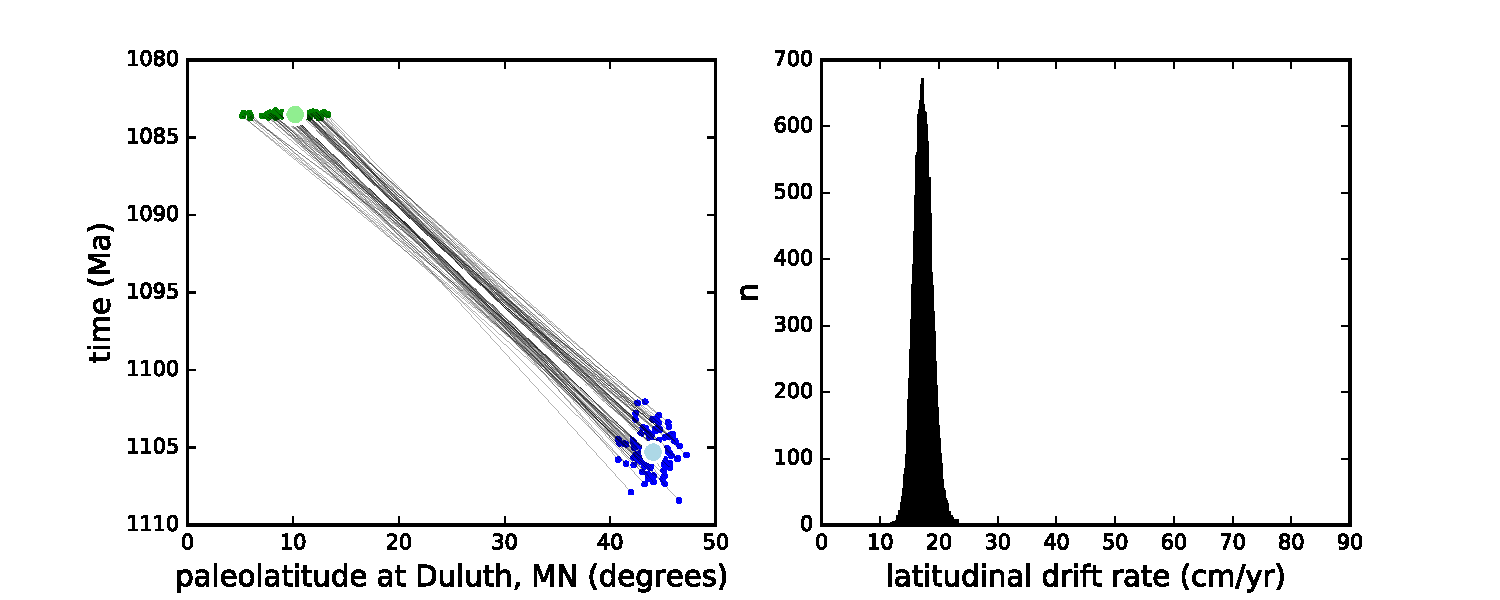
\includegraphics{Late_Rift_Data_Analysis_files/OslerMichipicoten_3.pdf}
    \adjustimage{max size={\linewidth}{\paperheight}}{Late_Rift_Data_Analysis_files/OslerMichipicoten_3.pdf}
    \end{figure}
    
\noindent 2.5\textsuperscript{th} percentile is: 14.5 cm/yr\\
50\textsuperscript{th} percentile is: 17.3 cm/yr\\
97.5\textsuperscript{th} percentile is: 20.4 cm/yr\\


\newpage

\subsubsection{Latitudinal motion implied by Mamainse lowerN/upperR and Michipicoten poles}\label{MamainseMichipicotenRate}

\begin{itemize}
\item{The paleolatitude for reference location (Duluth, MN) resulting from pole 1 (Mamainse Point lowerN/upperR) is: 32.9\textdegree}
\item{The paleolatitude for reference location (Duluth, MN) resulting from pole 2 (Michipicoten Island Formation) is: 10.2\textdegree}
\item{The rate of paleolatitudinal change implied by the poles pairs is: 14.9 cm/yr}
\end{itemize}

    \begin{center}
    \adjustimage{max size={0.6\linewidth}{0.6\paperheight}}{Late_Rift_Data_Analysis_files/MamainseMichipicoten_1.pdf}
    \end{center}
    
    \begin{figure}[h]
    \centering
%    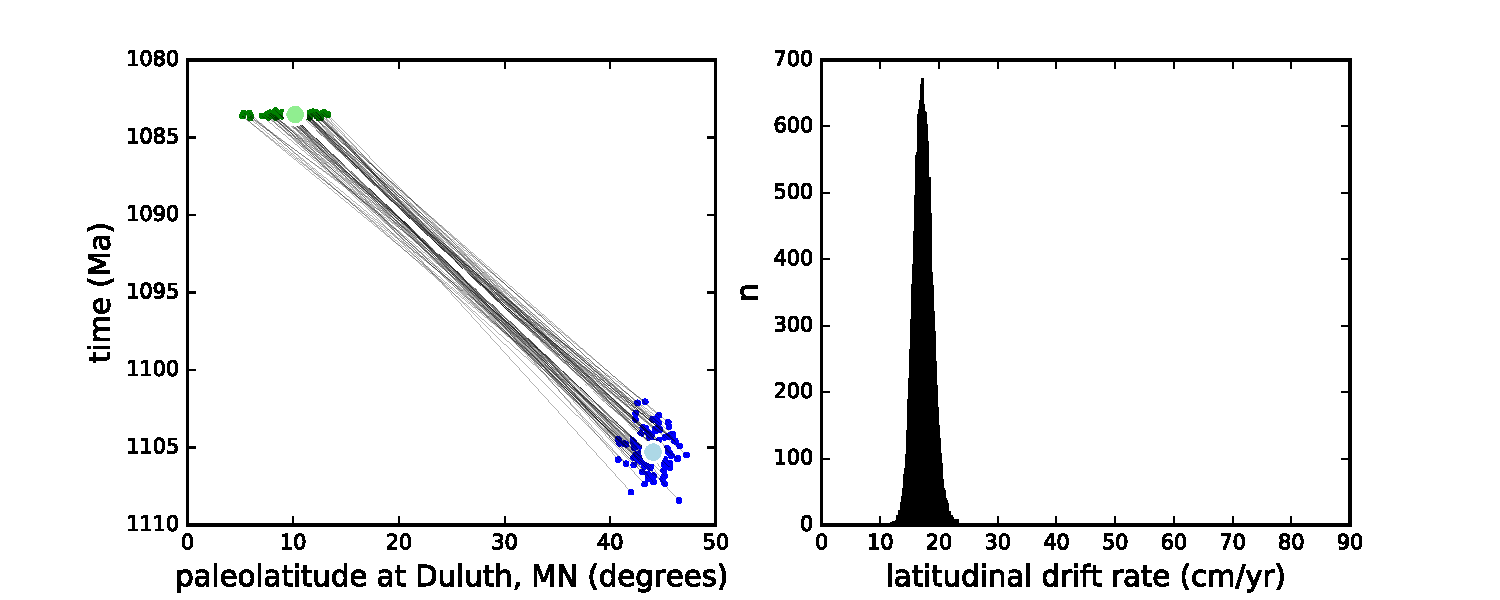
\includegraphics{Late_Rift_Data_Analysis_files/OslerMichipicoten_3.pdf}
    \adjustimage{max size={\linewidth}{\paperheight}}{Late_Rift_Data_Analysis_files/MamainseMichipicoten_3.pdf}
    \end{figure}
    
\noindent 2.5\textsuperscript{th} percentile is: 11.6 cm/yr\\
50\textsuperscript{th} percentile is: 14.9 cm/yr\\
97.5\textsuperscript{th} percentile is: 18.3 cm/yr\\
    
\newpage

\subsubsection{Latitudinal motion implied by North Shore Volcanic Group and Michipicoten poles}\label{MamainseMichipicotenRate}

\begin{itemize}
\item{The paleolatitude for reference location (Duluth, MN) resulting from pole 1 (North Shore Volcanic Group) is: 27.8\textdegree}
\item{The paleolatitude for reference location (Duluth, MN) resulting from pole 2 (Michipicoten Island Formation) is: 10.2\textdegree}
\item{The rate of paleolatitudinal change implied by the poles pairs is: 18.3 cm/yr}
\end{itemize}

    \begin{center}
    \adjustimage{max size={0.6\linewidth}{0.6\paperheight}}{Late_Rift_Data_Analysis_files/NSVGMichipicoten_1.pdf}
    \end{center}
    
    \begin{figure}[h]
    \centering
%    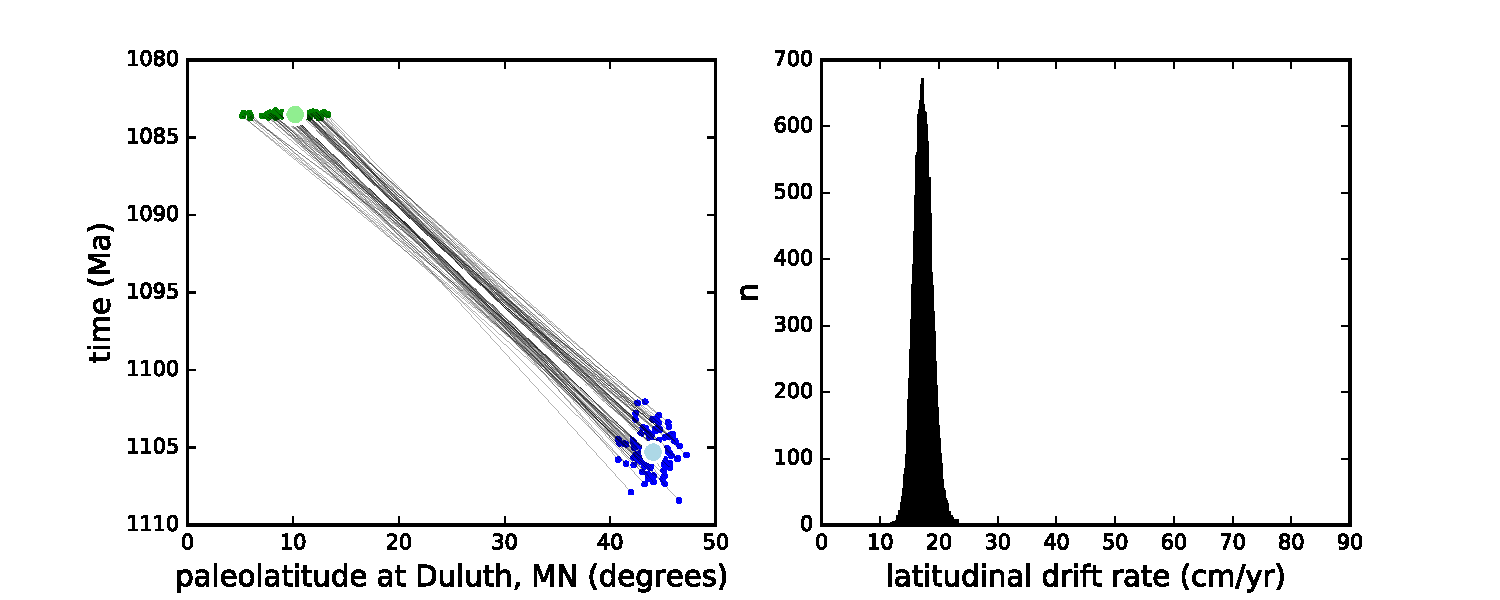
\includegraphics{Late_Rift_Data_Analysis_files/OslerMichipicoten_3.pdf}
    \adjustimage{max size={\linewidth}{\paperheight}}{Late_Rift_Data_Analysis_files/NSVGMichipicoten_3.pdf}
    \end{figure}
    
\noindent 2.5\textsuperscript{th} percentile is: 13.9 cm/yr\\
50\textsuperscript{th} percentile is: 18.3 cm/yr\\
97.5\textsuperscript{th} percentile is: 22.8 cm/yr\\

\newpage


    
    \subsection{Age of Keweenawan
sediments}\label{age-of-keweenawan-sediments}

\subsubsection{\texorpdfstring{\textit{Nonesuch
Shale}}{Nonesuch Shale}}\label{nonesuch-shale}

Geological evidence supports the interpretation that the deposition of the Nonesuch Shale occured shortly after or perhaps during late stage volcanism in the Midcontinent Rift (see main text). However, the magnetization of this formation
cannot be dated as definitively. \cite{Symons2013a} suggested that the
magnetization of the Nonesuch shale is secondary, likely a product of
oxidation and mineralization in the Nonesuch Formation that postdates
its deposition and subsequent burial by the Freda sandstone. They dated
this magnetization at 1063 \(\pm\) 8 Ma by projecting Laurentia's
latitudinal rate of motion to the paleolatitude implied by the Nonesuch
paleomagnetic pole. Their analysis assumes a rate of motion consistent
with the previously hypothesized slowdown of Laurentia during the late
stage of rifting \citep{Davis1997a}. However, our results suggest
no significant change in Laurentia's motion over this period. Redoing
the analysis of \cite{Symons2013a} with our revised rate estimates
yields an age of Nonesuch shale magnetization of approximately 1078 Ma
(see below).

    Create a motion path of Laurentia that captures the paleolatitude of
Duluth, MN at 5 myr intervals through active rifting (1108-1083 Ma).

    \begin{Verbatim}[commandchars=\\\{\}]
{\color{incolor}In [{\color{incolor}54}]:} \PY{c+c1}{\PYZsh{} Duluth, MN}
         \PY{n}{SeedPoint} \PY{o}{=} \PY{p}{(}\PY{l+m+mf}{46.78}\PY{p}{,}\PY{o}{\PYZhy{}}\PY{l+m+mf}{92.1}\PY{p}{)}
         \PY{n}{MovingPlate} \PY{o}{=} \PY{l+m+mi}{1000}
         \PY{n}{RelativePlate} \PY{o}{=} \PY{l+m+mi}{0}
         \PY{n}{times} \PY{o}{=} \PY{n}{np}\PY{o}{.}\PY{n}{arange}\PY{p}{(}\PY{l+m+mi}{1083}\PY{p}{,}\PY{l+m+mi}{1108}\PY{p}{,}\PY{l+m+mi}{5}\PY{p}{)}
         
         \PY{c+c1}{\PYZsh{} Create a motion path feature}
         \PY{n}{digitisation\PYZus{}time} \PY{o}{=} \PY{l+m+mi}{0}
         \PY{n}{seed\PYZus{}points\PYZus{}at\PYZus{}digitisation\PYZus{}time} \PY{o}{=} \PY{n}{pygplates}\PY{o}{.}\PY{n}{MultiPointOnSphere}\PY{p}{(}\PY{p}{[}\PY{n}{SeedPoint}\PY{p}{]}\PY{p}{)} 
         \PY{n}{motion\PYZus{}path\PYZus{}feature} \PY{o}{=} \PY{n}{pygplates}\PY{o}{.}\PY{n}{Feature}\PY{o}{.}\PY{n}{create\PYZus{}motion\PYZus{}path}\PY{p}{(}
                 \PY{n}{seed\PYZus{}points\PYZus{}at\PYZus{}digitisation\PYZus{}time}\PY{p}{,}
                 \PY{n}{times}\PY{p}{,}
                 \PY{n}{valid\PYZus{}time}\PY{o}{=}\PY{p}{(}\PY{l+m+mi}{1110}\PY{p}{,} \PY{l+m+mi}{1000}\PY{p}{)}\PY{p}{,}
                 \PY{n}{relative\PYZus{}plate}\PY{o}{=}\PY{n}{RelativePlate}\PY{p}{,}
                 \PY{n}{reconstruction\PYZus{}plate\PYZus{}id} \PY{o}{=} \PY{n}{MovingPlate}\PY{p}{)}
         
         \PY{c+c1}{\PYZsh{} Create the shape of the motion path}
         \PY{n}{reconstruction\PYZus{}time} \PY{o}{=} \PY{l+m+mi}{1083}
         \PY{n}{reconstructed\PYZus{}motion\PYZus{}paths} \PY{o}{=} \PY{p}{[}\PY{p}{]}
         \PY{n}{pygplates}\PY{o}{.}\PY{n}{reconstruct}\PY{p}{(}\PY{n}{motion\PYZus{}path\PYZus{}feature}\PY{p}{,} \PY{n}{rotation\PYZus{}model}\PY{p}{,} 
                               \PY{n}{reconstructed\PYZus{}motion\PYZus{}paths}\PY{p}{,} \PY{n}{reconstruction\PYZus{}time}\PY{p}{,}
                               \PY{n}{reconstruct\PYZus{}type}\PY{o}{=}\PY{n}{pygplates}\PY{o}{.}\PY{n}{ReconstructType}\PY{o}{.}\PY{n}{motion\PYZus{}path}\PY{p}{)}
         
         \PY{c+c1}{\PYZsh{} get the reconstructed coordinates into numpy arrays}
         \PY{k}{for} \PY{n}{reconstructed\PYZus{}motion\PYZus{}path} \PY{o+ow}{in} \PY{n}{reconstructed\PYZus{}motion\PYZus{}paths}\PY{p}{:}
             \PY{n}{trail} \PY{o}{=} \PY{n}{reconstructed\PYZus{}motion\PYZus{}path}\PY{o}{.}\PY{n}{get\PYZus{}motion\PYZus{}path}\PY{p}{(}\PY{p}{)}\PY{o}{.}\PY{n}{to\PYZus{}lat\PYZus{}lon\PYZus{}array}\PY{p}{(}\PY{p}{)}
\end{Verbatim}

    \begin{Verbatim}[commandchars=\\\{\}]
{\color{incolor}In [{\color{incolor}55}]:} \PY{n}{plt}\PY{o}{.}\PY{n}{plot}\PY{p}{(}\PY{n}{times}\PY{p}{,}\PY{n}{np}\PY{o}{.}\PY{n}{flipud}\PY{p}{(}\PY{n}{trail}\PY{p}{[}\PY{p}{:}\PY{p}{,}\PY{l+m+mi}{0}\PY{p}{]}\PY{p}{)}\PY{p}{)}
         \PY{n}{plt}\PY{o}{.}\PY{n}{title}\PY{p}{(}\PY{l+s+s1}{\PYZsq{}}\PY{l+s+s1}{Paleolatitude of Duluth, MN}\PY{l+s+s1}{\PYZsq{}}\PY{p}{)}
         \PY{n}{plt}\PY{o}{.}\PY{n}{xlabel}\PY{p}{(}\PY{l+s+s1}{\PYZsq{}}\PY{l+s+s1}{Time (Ma)}\PY{l+s+s1}{\PYZsq{}}\PY{p}{)}
         \PY{n}{plt}\PY{o}{.}\PY{n}{ylabel}\PY{p}{(}\PY{l+s+s1}{\PYZsq{}}\PY{l+s+s1}{Latitude}\PY{l+s+s1}{\PYZsq{}}\PY{p}{)}
         \PY{n}{plt}\PY{o}{.}\PY{n}{gca}\PY{p}{(}\PY{p}{)}\PY{o}{.}\PY{n}{grid}\PY{p}{(}\PY{p}{)}
         \PY{n}{plt}\PY{o}{.}\PY{n}{gca}\PY{p}{(}\PY{p}{)}\PY{o}{.}\PY{n}{invert\PYZus{}xaxis}\PY{p}{(}\PY{p}{)}
         \PY{n}{plt}\PY{o}{.}\PY{n}{show}\PY{p}{(}\PY{p}{)}
\end{Verbatim}

    \begin{center}
    \adjustimage{max size={0.6\linewidth}{0.6\paperheight}}{Late_Rift_Data_Analysis_files/Late_Rift_Data_Analysis_88_0.pdf}
    \end{center}
    
    The latitudinal change plotted above appears fairly constant. We
therefore make a least squares fit to this data below.

    \begin{Verbatim}[commandchars=\\\{\}]
{\color{incolor}In [{\color{incolor}56}]:} \PY{n}{m}\PY{p}{,} \PY{n}{c} \PY{o}{=} \PY{n}{np}\PY{o}{.}\PY{n}{linalg}\PY{o}{.}\PY{n}{lstsq}\PY{p}{(}\PY{n}{np}\PY{o}{.}\PY{n}{vstack}\PY{p}{(}\PY{p}{[}\PY{n}{times}\PY{p}{,} \PY{n}{np}\PY{o}{.}\PY{n}{ones}\PY{p}{(}\PY{n+nb}{len}\PY{p}{(}\PY{n}{times}\PY{p}{)}\PY{p}{)}\PY{p}{]}\PY{p}{)}\PY{o}{.}\PY{n}{T}\PY{p}{,}
                                \PY{n}{np}\PY{o}{.}\PY{n}{flipud}\PY{p}{(}\PY{n}{trail}\PY{p}{[}\PY{p}{:}\PY{p}{,}\PY{l+m+mi}{0}\PY{p}{]}\PY{p}{)}\PY{p}{)}\PY{p}{[}\PY{l+m+mi}{0}\PY{p}{]}
         \PY{k}{print} \PY{l+s+s1}{\PYZsq{}}\PY{l+s+s1}{Rate of Laurentia}\PY{l+s+se}{\PYZbs{}\PYZsq{}}\PY{l+s+s1}{s latitudinal motion = }\PY{l+s+si}{\PYZpc{}0.4f}\PY{l+s+s1}{ degrees/myr}\PY{l+s+s1}{\PYZsq{}} \PY{o}{\PYZpc{}} \PY{p}{(}\PY{n}{m}\PY{p}{)}
         \PY{k}{print} \PY{l+s+s1}{\PYZsq{}}\PY{l+s+s1}{or }\PY{l+s+si}{\PYZpc{}0.4f}\PY{l+s+s1}{ cm/yr}\PY{l+s+s1}{\PYZsq{}} \PY{o}{\PYZpc{}} \PY{p}{(}\PY{n}{m}\PY{o}{*}\PY{l+m+mf}{11.132}\PY{p}{)}
\end{Verbatim}

    \begin{Verbatim}[commandchars=\\\{\}]
Rate of Laurentia's latitudinal motion = 1.3767 degrees/myr
or 15.3254 cm/yr
    \end{Verbatim}

    \begin{Verbatim}[commandchars=\\\{\}]
{\color{incolor}In [{\color{incolor}57}]:} \PY{n}{plt}\PY{o}{.}\PY{n}{plot}\PY{p}{(}\PY{n}{times}\PY{p}{,}\PY{n}{np}\PY{o}{.}\PY{n}{flipud}\PY{p}{(}\PY{n}{trail}\PY{p}{[}\PY{p}{:}\PY{p}{,}\PY{l+m+mi}{0}\PY{p}{]}\PY{p}{)}\PY{p}{)}
         \PY{n}{times\PYZus{}new} \PY{o}{=} \PY{n}{np}\PY{o}{.}\PY{n}{arange}\PY{p}{(}\PY{l+m+mi}{1073}\PY{p}{,}\PY{l+m+mi}{1108}\PY{p}{,}\PY{l+m+mi}{5}\PY{p}{)}
         \PY{n}{plt}\PY{o}{.}\PY{n}{plot}\PY{p}{(}\PY{n}{times\PYZus{}new}\PY{p}{,} \PY{n}{m}\PY{o}{*}\PY{n}{times\PYZus{}new} \PY{o}{+} \PY{n}{c}\PY{p}{,} \PY{l+s+s1}{\PYZsq{}}\PY{l+s+s1}{r}\PY{l+s+s1}{\PYZsq{}}\PY{p}{)}
         \PY{c+c1}{\PYZsh{} Paleolatitude of Nonesuch is 5.6 degrees}
         \PY{n}{plt}\PY{o}{.}\PY{n}{plot}\PY{p}{(}\PY{p}{[}\PY{l+m+mi}{1070}\PY{p}{,}\PY{l+m+mi}{1105}\PY{p}{]}\PY{p}{,} \PY{p}{[}\PY{l+m+mf}{5.6}\PY{p}{,}\PY{l+m+mf}{5.6}\PY{p}{]}\PY{p}{)}
         \PY{n}{NS\PYZus{}inferred\PYZus{}age} \PY{o}{=} \PY{p}{(}\PY{l+m+mf}{5.6}\PY{o}{\PYZhy{}}\PY{n}{c}\PY{p}{)}\PY{o}{/}\PY{n}{m}
         \PY{n}{plt}\PY{o}{.}\PY{n}{title}\PY{p}{(}\PY{l+s+s1}{\PYZsq{}}\PY{l+s+s1}{Paleolatitude of Duluth, MN}\PY{l+s+s1}{\PYZsq{}}\PY{p}{)}
         \PY{n}{plt}\PY{o}{.}\PY{n}{xlabel}\PY{p}{(}\PY{l+s+s1}{\PYZsq{}}\PY{l+s+s1}{Time (Ma)}\PY{l+s+s1}{\PYZsq{}}\PY{p}{)}
         \PY{n}{plt}\PY{o}{.}\PY{n}{ylabel}\PY{p}{(}\PY{l+s+s1}{\PYZsq{}}\PY{l+s+s1}{Latitude}\PY{l+s+s1}{\PYZsq{}}\PY{p}{)}
         \PY{n}{plt}\PY{o}{.}\PY{n}{gca}\PY{p}{(}\PY{p}{)}\PY{o}{.}\PY{n}{grid}\PY{p}{(}\PY{p}{)}
         \PY{n}{plt}\PY{o}{.}\PY{n}{gca}\PY{p}{(}\PY{p}{)}\PY{o}{.}\PY{n}{invert\PYZus{}xaxis}\PY{p}{(}\PY{p}{)}
         \PY{n}{plt}\PY{o}{.}\PY{n}{show}\PY{p}{(}\PY{p}{)}
\end{Verbatim}

    \begin{Verbatim}[commandchars=\\\{\}]
Inferred age of Nonesuch Shale if Laurentia
continued moving at the same rate after Midcontinent Rift volcanism ended:
1078.4340 Ma
    \end{Verbatim}

    \begin{center}
    \adjustimage{max size={0.6\linewidth}{0.6\paperheight}}{Late_Rift_Data_Analysis_files/Late_Rift_Data_Analysis_91_1.pdf}
    \end{center}
    
    \subsubsection{\texorpdfstring{\textit{Jacobsville
Sandstone}}{Jacobsville Sandstone}}\label{jacobsville-sandstone}

    New detrital zircon dates from the Jacobsville sandstone, which
unconformably overlies the Freda sandstone, reveal a much younger age
for this formation than estimated for the Oronto Group sediments
($<$959 \(\pm\) 19 Ma; \citealp{Malone2016a}). The
paleolatitude of Laurentia implied by the Neoproterozoic APWP was then
matched with that implied by the Jacobsville paleomagnetic pole,
yielding a set of possible ages for Jacobsville deposition:
$\sim$780-755, $\sim$700-610 or $\sim$570-555 Ma \citep{Malone2016a}. Motivations for
redoing this analysis with paleomagnetic poles from both the APWP of
Laurentia and the APWP of Baltica (hypothesized to have a longstanding
connection with Laurentia's northeastern margin throughout the
Neoproterozoic; \citealp{Pisarevsky2003a}; \citealp{Li2008a}; \citealp{Evans2009a})
are outlined in the main text (\textit{Discussion: Age of Keweenawan
sediments}).

We first upload paleomagnetic poles of Laurentia as compiled by the
Nordic Supercontinent Workshop, Haraldvangen, Norway in 2014 (see
references in Figure 7 of the manuscript).

    \begin{Verbatim}[commandchars=\\\{\}]
{\color{incolor}In [{\color{incolor}58}]:} \PY{n}{Laurentia\PYZus{}poles} \PY{o}{=} \PY{n}{pd}\PY{o}{.}\PY{n}{read\PYZus{}csv}\PY{p}{(}\PY{l+s+s1}{\PYZsq{}}\PY{l+s+s1}{../Data/Reconstruction/Laurentia\PYZus{}Poles.csv}\PY{l+s+s1}{\PYZsq{}}\PY{p}{,} 
                                       \PY{n}{usecols}\PY{o}{=}\PY{p}{[}\PY{l+s+s1}{\PYZsq{}}\PY{l+s+s1}{Formation}\PY{l+s+s1}{\PYZsq{}}\PY{p}{,} \PY{l+s+s1}{\PYZsq{}}\PY{l+s+s1}{Terrane}\PY{l+s+s1}{\PYZsq{}}\PY{p}{,} \PY{l+s+s1}{\PYZsq{}}\PY{l+s+s1}{AgeUpper}\PY{l+s+s1}{\PYZsq{}}\PY{p}{,} 
                                                \PY{l+s+s1}{\PYZsq{}}\PY{l+s+s1}{AgeLower}\PY{l+s+s1}{\PYZsq{}}\PY{p}{,} \PY{l+s+s1}{\PYZsq{}}\PY{l+s+s1}{AgeNominal}\PY{l+s+s1}{\PYZsq{}}\PY{p}{,} \PY{l+s+s1}{\PYZsq{}}\PY{l+s+s1}{A95}\PY{l+s+s1}{\PYZsq{}}\PY{p}{,} 
                                                \PY{l+s+s1}{\PYZsq{}}\PY{l+s+s1}{SLat}\PY{l+s+s1}{\PYZsq{}}\PY{p}{,} \PY{l+s+s1}{\PYZsq{}}\PY{l+s+s1}{SLon}\PY{l+s+s1}{\PYZsq{}}\PY{p}{,} \PY{l+s+s1}{\PYZsq{}}\PY{l+s+s1}{PLat}\PY{l+s+s1}{\PYZsq{}}\PY{p}{,} \PY{l+s+s1}{\PYZsq{}}\PY{l+s+s1}{PLon}\PY{l+s+s1}{\PYZsq{}}\PY{p}{,} 
                                                \PY{l+s+s1}{\PYZsq{}}\PY{l+s+s1}{RefLat}\PY{l+s+s1}{\PYZsq{}}\PY{p}{,} \PY{l+s+s1}{\PYZsq{}}\PY{l+s+s1}{RefLon}\PY{l+s+s1}{\PYZsq{}}\PY{p}{]}\PY{p}{)}
         \PY{n}{Laurentia\PYZus{}poles} \PY{o}{=} \PY{n}{Laurentia\PYZus{}poles}\PY{o}{.}\PY{n}{sort\PYZus{}values}\PY{p}{(}\PY{n}{by}\PY{o}{=}\PY{l+s+s1}{\PYZsq{}}\PY{l+s+s1}{AgeNominal}\PY{l+s+s1}{\PYZsq{}}\PY{p}{,} 
                                                       \PY{n}{ascending}\PY{o}{=}\PY{n+nb+bp}{False}\PY{p}{)}
         \PY{n}{Laurentia\PYZus{}poles}\PY{o}{.}\PY{n}{reset\PYZus{}index}\PY{p}{(}\PY{n}{inplace}\PY{o}{=}\PY{n+nb+bp}{True}\PY{p}{,} \PY{n}{drop}\PY{o}{=}\PY{n+nb+bp}{True}\PY{p}{)}
         \PY{n}{Laurentia\PYZus{}poles}
\end{Verbatim}

%\begin{Verbatim}[commandchars=\\\{\}]
%{\color{outcolor}Out[{\color{outcolor}58}]:} \href{run:../Data/Reconstruction/Laurentia_Poles.csv}{Click to view Laurentia poles}
%        (as compiled by the 2014 Nordic Supercontinent Workshop, Haraldvangen, Norway,
%        and with additional data from this study)
%\end{Verbatim}
\noindent These paleomagnetic data (as compiled by the 2014 Nordic Supercontinent Workshop, Haraldvangen, Norway, and with additional data from this study) can be found in the Data Repository under \texttt{/Data/Reconstruction/Laurentia\_Poles.csv}.\\      

        
    The paleolatitude of Duluth, MN (``RefLat'', ``RefLon'') is then
calculated for each of these paleomagnetic poles and plotted below.

    \begin{Verbatim}[commandchars=\\\{\}]
{\color{incolor}In [{\color{incolor}59}]:} \PY{n}{Laurentia\PYZus{}poles}\PY{p}{[}\PY{l+s+s1}{\PYZsq{}}\PY{l+s+s1}{Latitude}\PY{l+s+s1}{\PYZsq{}}\PY{p}{]} \PY{o}{=} \PY{n}{pd}\PY{o}{.}\PY{n}{Series}\PY{p}{(}\PY{l+m+mi}{90} \PY{o}{\PYZhy{}} \PY{n}{np}\PY{o}{.}\PY{n}{rad2deg}\PY{p}{(}\PY{n}{np}\PY{o}{.}\PY{n}{arccos}\PYZbs{}
         \PY{p}{(}\PY{n}{np}\PY{o}{.}\PY{n}{sin}\PY{p}{(}\PY{n}{np}\PY{o}{.}\PY{n}{deg2rad}\PY{p}{(}\PY{n}{Laurentia\PYZus{}poles}\PY{p}{[}\PY{l+s+s1}{\PYZsq{}}\PY{l+s+s1}{RefLat}\PY{l+s+s1}{\PYZsq{}}\PY{p}{]}\PY{p}{)}\PY{p}{)}\PYZbs{}
         \PY{o}{*}\PY{n}{np}\PY{o}{.}\PY{n}{sin}\PY{p}{(}\PY{n}{np}\PY{o}{.}\PY{n}{deg2rad}\PY{p}{(}\PY{n}{Laurentia\PYZus{}poles}\PY{p}{[}\PY{l+s+s1}{\PYZsq{}}\PY{l+s+s1}{PLat}\PY{l+s+s1}{\PYZsq{}}\PY{p}{]}\PY{p}{)}\PY{p}{)}\PYZbs{}
         \PY{o}{+}\PY{n}{np}\PY{o}{.}\PY{n}{cos}\PY{p}{(}\PY{n}{np}\PY{o}{.}\PY{n}{deg2rad}\PY{p}{(}\PY{n}{Laurentia\PYZus{}poles}\PY{p}{[}\PY{l+s+s1}{\PYZsq{}}\PY{l+s+s1}{RefLat}\PY{l+s+s1}{\PYZsq{}}\PY{p}{]}\PY{p}{)}\PY{p}{)}\PYZbs{}
         \PY{o}{*}\PY{n}{np}\PY{o}{.}\PY{n}{cos}\PY{p}{(}\PY{n}{np}\PY{o}{.}\PY{n}{deg2rad}\PY{p}{(}\PY{n}{Laurentia\PYZus{}poles}\PY{p}{[}\PY{l+s+s1}{\PYZsq{}}\PY{l+s+s1}{PLat}\PY{l+s+s1}{\PYZsq{}}\PY{p}{]}\PY{p}{)}\PY{p}{)}\PYZbs{}
         \PY{o}{*}\PY{n}{np}\PY{o}{.}\PY{n}{cos}\PY{p}{(}\PY{n}{np}\PY{o}{.}\PY{n}{deg2rad}\PY{p}{(}\PY{n}{Laurentia\PYZus{}poles}\PY{p}{[}\PY{l+s+s1}{\PYZsq{}}\PY{l+s+s1}{RefLon}\PY{l+s+s1}{\PYZsq{}}\PY{p}{]}\PY{o}{\PYZhy{}}\PY{n}{Laurentia\PYZus{}poles}\PY{p}{[}\PY{l+s+s1}{\PYZsq{}}\PY{l+s+s1}{PLon}\PY{l+s+s1}{\PYZsq{}}\PY{p}{]}\PY{p}{)}\PY{p}{)}\PY{p}{)}\PY{p}{)}\PY{p}{)}
\end{Verbatim}

    \begin{Verbatim}[commandchars=\\\{\}]
{\color{incolor}In [{\color{incolor}60}]:} \PY{c+c1}{\PYZsh{} First we must tweak the format of the pole list}
         \PY{n}{Laurentia\PYZus{}copy} \PY{o}{=} \PY{n}{pd}\PY{o}{.}\PY{n}{DataFrame}\PY{p}{(}\PY{n}{Laurentia\PYZus{}poles}\PY{p}{,} \PY{n}{columns}\PY{o}{=}\PY{p}{[}\PY{l+s+s1}{\PYZsq{}}\PY{l+s+s1}{PLat}\PY{l+s+s1}{\PYZsq{}}\PY{p}{,}\PY{l+s+s1}{\PYZsq{}}\PY{l+s+s1}{PLon}\PY{l+s+s1}{\PYZsq{}}\PY{p}{]}\PY{p}{)}
         \PY{n}{Laurentia\PYZus{}copy} \PY{o}{=} \PY{n}{Laurentia\PYZus{}copy}\PY{o}{.}\PY{n}{rename\PYZus{}axis}\PY{p}{(}\PY{p}{\PYZob{}}\PY{l+s+s1}{\PYZsq{}}\PY{l+s+s1}{PLat}\PY{l+s+s1}{\PYZsq{}}\PY{p}{:}\PY{l+s+s1}{\PYZsq{}}\PY{l+s+s1}{PLat\PYZus{}rot}\PY{l+s+s1}{\PYZsq{}}\PY{p}{,} 
                                                      \PY{l+s+s1}{\PYZsq{}}\PY{l+s+s1}{PLon}\PY{l+s+s1}{\PYZsq{}}\PY{p}{:}\PY{l+s+s1}{\PYZsq{}}\PY{l+s+s1}{PLon\PYZus{}rot}\PY{l+s+s1}{\PYZsq{}}\PY{p}{\PYZcb{}}\PY{p}{,} 
                                                     \PY{n}{axis}\PY{o}{=}\PY{l+s+s1}{\PYZsq{}}\PY{l+s+s1}{columns}\PY{l+s+s1}{\PYZsq{}}\PY{p}{)}
         \PY{n}{Laurentia\PYZus{}poles}\PY{p}{[}\PY{l+s+s1}{\PYZsq{}}\PY{l+s+s1}{PLat\PYZus{}rot}\PY{l+s+s1}{\PYZsq{}}\PY{p}{]} \PY{o}{=} \PY{n}{Laurentia\PYZus{}copy}\PY{o}{.}\PY{n}{PLat\PYZus{}rot}
         \PY{n}{Laurentia\PYZus{}poles}\PY{p}{[}\PY{l+s+s1}{\PYZsq{}}\PY{l+s+s1}{PLon\PYZus{}rot}\PY{l+s+s1}{\PYZsq{}}\PY{p}{]} \PY{o}{=} \PY{n}{Laurentia\PYZus{}copy}\PY{o}{.}\PY{n}{PLon\PYZus{}rot}
         \PY{n}{Laurentia\PYZus{}poles}\PY{p}{[}\PY{l+s+s1}{\PYZsq{}}\PY{l+s+s1}{AgeNominal\PYZus{}neg}\PY{l+s+s1}{\PYZsq{}}\PY{p}{]} \PY{o}{=} \PY{n}{Laurentia\PYZus{}poles}\PY{o}{.}\PY{n}{AgeNominal}\PY{o}{.}\PY{n}{apply}\PY{p}{(}\PY{n}{np}\PY{o}{.}\PY{n}{negative}\PY{p}{)}
         
         \PY{c+c1}{\PYZsh{} Plot the paleolatitude of Duluth using Laurentia poles}
         \PY{n}{fig} \PY{o}{=} \PY{n}{plt}\PY{o}{.}\PY{n}{figure}\PY{p}{(}\PY{n}{figsize}\PY{o}{=}\PY{p}{(}\PY{l+m+mi}{20}\PY{p}{,}\PY{l+m+mi}{6}\PY{p}{)}\PY{p}{)}
         
         \PY{n}{ax1} \PY{o}{=} \PY{n}{fig}\PY{o}{.}\PY{n}{add\PYZus{}subplot}\PY{p}{(}\PY{l+m+mi}{131}\PY{p}{)}
         \PY{n}{ax1}\PY{o}{.}\PY{n}{add\PYZus{}patch}\PY{p}{(}\PY{n}{mpatch}\PY{o}{.}\PY{n}{Rectangle}\PY{p}{(}\PY{p}{(}\PY{l+m+mi}{1300}\PY{p}{,} \PY{o}{\PYZhy{}}\PY{l+m+mf}{12.2}\PY{p}{)}\PY{p}{,} \PY{o}{\PYZhy{}}\PY{l+m+mi}{1000}\PY{p}{,} \PY{l+m+mf}{8.4}\PY{p}{,} 
                                        \PY{n}{facecolor}\PY{o}{=}\PY{l+s+s1}{\PYZsq{}}\PY{l+s+s1}{r}\PY{l+s+s1}{\PYZsq{}}\PY{p}{,} \PY{n}{alpha}\PY{o}{=}\PY{l+m+mf}{0.2}\PY{p}{)}\PY{p}{)}
         \PY{n}{ax1}\PY{o}{.}\PY{n}{plot}\PY{p}{(}\PY{p}{[}\PY{o}{\PYZhy{}}\PY{l+m+mf}{8.1}\PY{p}{]}\PY{o}{*}\PY{l+m+mi}{2000}\PY{p}{,} \PY{l+s+s1}{\PYZsq{}}\PY{l+s+s1}{r\PYZhy{}}\PY{l+s+s1}{\PYZsq{}}\PY{p}{)}
         \PY{n}{ax1}\PY{o}{.}\PY{n}{errorbar}\PY{p}{(}\PY{n}{Laurentia\PYZus{}poles}\PY{p}{[}\PY{l+s+s1}{\PYZsq{}}\PY{l+s+s1}{AgeNominal}\PY{l+s+s1}{\PYZsq{}}\PY{p}{]}\PY{o}{.}\PY{n}{tolist}\PY{p}{(}\PY{p}{)}\PY{p}{,} 
                      \PY{n}{Laurentia\PYZus{}poles}\PY{p}{[}\PY{l+s+s1}{\PYZsq{}}\PY{l+s+s1}{Latitude}\PY{l+s+s1}{\PYZsq{}}\PY{p}{]}\PY{o}{.}\PY{n}{tolist}\PY{p}{(}\PY{p}{)}\PY{p}{,} 
                      \PY{n}{yerr}\PY{o}{=}\PY{n}{Laurentia\PYZus{}poles}\PY{p}{[}\PY{l+s+s1}{\PYZsq{}}\PY{l+s+s1}{A95}\PY{l+s+s1}{\PYZsq{}}\PY{p}{]}\PY{o}{.}\PY{n}{tolist}\PY{p}{(}\PY{p}{)}\PY{p}{,} 
                      \PY{n}{xerr}\PY{o}{=}\PY{p}{(}\PY{n}{Laurentia\PYZus{}poles}\PY{p}{[}\PY{l+s+s1}{\PYZsq{}}\PY{l+s+s1}{AgeUpper}\PY{l+s+s1}{\PYZsq{}}\PY{p}{]}\PY{o}{\PYZhy{}}\PY{n}{Laurentia\PYZus{}poles}\PY{p}{[}\PY{l+s+s1}{\PYZsq{}}\PY{l+s+s1}{AgeLower}\PY{l+s+s1}{\PYZsq{}}\PY{p}{]}\PY{p}{)}\PY{o}{/}\PY{l+m+mi}{2}\PY{p}{)}
         \PY{n}{ax1}\PY{o}{.}\PY{n}{text}\PY{p}{(}\PY{l+m+mi}{1150}\PY{p}{,} \PY{o}{\PYZhy{}}\PY{l+m+mi}{6}\PY{p}{,}\PY{l+s+s1}{\PYZsq{}}\PY{l+s+s1}{Paleolat. from Jacobsville Sandstone}\PY{l+s+s1}{\PYZsq{}}\PY{p}{,} 
                  \PY{n}{color}\PY{o}{=}\PY{l+s+s1}{\PYZsq{}}\PY{l+s+s1}{r}\PY{l+s+s1}{\PYZsq{}}\PY{p}{,} \PY{n}{withdash}\PY{o}{=}\PY{n+nb+bp}{True}\PY{p}{)}
         \PY{c+c1}{\PYZsh{} Cut off at Tonian/Cryogenian boundary}
         \PY{n}{ax1}\PY{o}{.}\PY{n}{set\PYZus{}xlim}\PY{p}{(}\PY{l+m+mi}{1200}\PY{p}{,}\PY{l+m+mi}{717}\PY{p}{)}
         \PY{n}{ax1}\PY{o}{.}\PY{n}{set\PYZus{}ylim}\PY{p}{(}\PY{o}{\PYZhy{}}\PY{l+m+mi}{90}\PY{p}{,}\PY{l+m+mi}{90}\PY{p}{)}
         \PY{n}{ax1}\PY{o}{.}\PY{n}{set\PYZus{}ylabel}\PY{p}{(}\PY{l+s+s1}{\PYZsq{}}\PY{l+s+s1}{Paleolatitude of Laurentia (Laurentia poles)}\PY{l+s+s1}{\PYZsq{}}\PY{p}{)}
         \PY{n}{ax1}\PY{o}{.}\PY{n}{set\PYZus{}xlabel}\PY{p}{(}\PY{l+s+s1}{\PYZsq{}}\PY{l+s+s1}{Age (Ma)}\PY{l+s+s1}{\PYZsq{}}\PY{p}{)}
         \PY{n}{plt}\PY{o}{.}\PY{n}{show}\PY{p}{(}\PY{p}{)}
\end{Verbatim}

    \begin{center}
    \adjustimage{max size={0.6\linewidth}{0.6\paperheight}}{Late_Rift_Data_Analysis_files/Late_Rift_Data_Analysis_97_0.pdf}
    \end{center}
    
    Next, we upload paleomagnetic poles of Baltica as compiled by the Nordic
Supercontinent Workshop, Haraldvangen, Norway in 2014 (see references in
Figure 7 of the manuscript).

    \begin{Verbatim}[commandchars=\\\{\}]
{\color{incolor}In [{\color{incolor}61}]:} \PY{n}{Baltica\PYZus{}poles} \PY{o}{=} \PY{n}{pd}\PY{o}{.}\PY{n}{read\PYZus{}csv}\PY{p}{(}\PY{l+s+s1}{\PYZsq{}}\PY{l+s+s1}{../Data/Reconstruction/Baltica\PYZus{}Poles.csv}\PY{l+s+s1}{\PYZsq{}}\PY{p}{,} 
                                       \PY{n}{usecols}\PY{o}{=}\PY{p}{[}\PY{l+s+s1}{\PYZsq{}}\PY{l+s+s1}{Formation}\PY{l+s+s1}{\PYZsq{}}\PY{p}{,} \PY{l+s+s1}{\PYZsq{}}\PY{l+s+s1}{Terrane}\PY{l+s+s1}{\PYZsq{}}\PY{p}{,} \PY{l+s+s1}{\PYZsq{}}\PY{l+s+s1}{AgeUpper}\PY{l+s+s1}{\PYZsq{}}\PY{p}{,} 
                                                \PY{l+s+s1}{\PYZsq{}}\PY{l+s+s1}{AgeLower}\PY{l+s+s1}{\PYZsq{}}\PY{p}{,} \PY{l+s+s1}{\PYZsq{}}\PY{l+s+s1}{AgeNominal}\PY{l+s+s1}{\PYZsq{}}\PY{p}{,} \PY{l+s+s1}{\PYZsq{}}\PY{l+s+s1}{A95}\PY{l+s+s1}{\PYZsq{}}\PY{p}{,} 
                                                \PY{l+s+s1}{\PYZsq{}}\PY{l+s+s1}{SLat}\PY{l+s+s1}{\PYZsq{}}\PY{p}{,} \PY{l+s+s1}{\PYZsq{}}\PY{l+s+s1}{SLon}\PY{l+s+s1}{\PYZsq{}}\PY{p}{,} \PY{l+s+s1}{\PYZsq{}}\PY{l+s+s1}{PLat}\PY{l+s+s1}{\PYZsq{}}\PY{p}{,} \PY{l+s+s1}{\PYZsq{}}\PY{l+s+s1}{PLon}\PY{l+s+s1}{\PYZsq{}}\PY{p}{,} 
                                                \PY{l+s+s1}{\PYZsq{}}\PY{l+s+s1}{RefLat}\PY{l+s+s1}{\PYZsq{}}\PY{p}{,} \PY{l+s+s1}{\PYZsq{}}\PY{l+s+s1}{RefLon}\PY{l+s+s1}{\PYZsq{}}\PY{p}{]}\PY{p}{)}
         \PY{n}{Baltica\PYZus{}poles} \PY{o}{=} \PY{n}{Baltica\PYZus{}poles}\PY{o}{.}\PY{n}{sort\PYZus{}values}\PY{p}{(}\PY{n}{by}\PY{o}{=}\PY{l+s+s1}{\PYZsq{}}\PY{l+s+s1}{AgeNominal}\PY{l+s+s1}{\PYZsq{}}\PY{p}{,} \PY{n}{ascending}\PY{o}{=}\PY{n+nb+bp}{False}\PY{p}{)}
         \PY{n}{Baltica\PYZus{}poles}\PY{o}{.}\PY{n}{reset\PYZus{}index}\PY{p}{(}\PY{n}{inplace}\PY{o}{=}\PY{n+nb+bp}{True}\PY{p}{,} \PY{n}{drop}\PY{o}{=}\PY{n+nb+bp}{True}\PY{p}{)}
         \PY{n}{Baltica\PYZus{}poles}
\end{Verbatim}

%            \begin{Verbatim}[commandchars=\\\{\}]
%{\color{outcolor}Out[{\color{outcolor}61}]:} \href{run:../Data/Reconstruction/Baltica_Poles.csv}{Click to view Baltica poles}
%        (as compiled by the 2014 Nordic Supercontinent Workshop, Haraldvangen, Norway)
%\end{Verbatim}
\noindent These paleomagnetic data (as compiled by the 2014 Nordic Supercontinent Workshop, Haraldvangen, Norway) can be found in the Data Repository under \texttt{/Data/Reconstruction/Baltica\_Poles.csv}.\\        
                                                    
    We then rotate these Baltica poles based on the reconstruction of Evans
(2009) and do the same calculation for paleolatitude of Duluth, MN.

    \begin{Verbatim}[commandchars=\\\{\}]
{\color{incolor}In [{\color{incolor}62}]:} \PY{n}{Baltica\PYZus{}poles}\PY{p}{[}\PY{l+s+s1}{\PYZsq{}}\PY{l+s+s1}{PLat\PYZus{}rot}\PY{l+s+s1}{\PYZsq{}}\PY{p}{]}\PY{p}{,} \PY{n}{Baltica\PYZus{}poles}\PY{p}{[}\PY{l+s+s1}{\PYZsq{}}\PY{l+s+s1}{PLon\PYZus{}rot}\PY{l+s+s1}{\PYZsq{}}\PY{p}{]} \PY{o}{=} \PY{n}{pmag}\PY{o}{.}\PY{n}{PTrot}\PY{p}{(}\PY{p}{[}\PY{l+m+mf}{81.5}\PY{p}{,} 
                                                                            \PY{o}{\PYZhy{}}\PY{l+m+mf}{110.0}\PY{p}{,}
                                                                            \PY{o}{\PYZhy{}}\PY{l+m+mf}{50.0}\PY{p}{]}\PY{p}{,} 
                                                \PY{n}{Baltica\PYZus{}poles}\PY{o}{.}\PY{n}{PLat}\PY{o}{.}\PY{n}{tolist}\PY{p}{(}\PY{p}{)}\PY{p}{,} 
                                                \PY{n}{Baltica\PYZus{}poles}\PY{o}{.}\PY{n}{PLon}\PY{o}{.}\PY{n}{tolist}\PY{p}{(}\PY{p}{)}\PY{p}{)}
         \PY{n}{Baltica\PYZus{}poles}\PY{p}{[}\PY{l+s+s1}{\PYZsq{}}\PY{l+s+s1}{Latitude}\PY{l+s+s1}{\PYZsq{}}\PY{p}{]} \PY{o}{=} \PY{n}{pd}\PY{o}{.}\PY{n}{Series}\PY{p}{(}\PY{l+m+mi}{90} \PY{o}{\PYZhy{}} \PY{n}{np}\PY{o}{.}\PY{n}{rad2deg}\PY{p}{(}\PY{n}{np}\PY{o}{.}\PY{n}{arccos}\PYZbs{}
         \PY{p}{(}\PY{n}{np}\PY{o}{.}\PY{n}{sin}\PY{p}{(}\PY{n}{np}\PY{o}{.}\PY{n}{deg2rad}\PY{p}{(}\PY{n}{Baltica\PYZus{}poles}\PY{p}{[}\PY{l+s+s1}{\PYZsq{}}\PY{l+s+s1}{RefLat}\PY{l+s+s1}{\PYZsq{}}\PY{p}{]}\PY{p}{)}\PY{p}{)}\PYZbs{}
         \PY{o}{*}\PY{n}{np}\PY{o}{.}\PY{n}{sin}\PY{p}{(}\PY{n}{np}\PY{o}{.}\PY{n}{deg2rad}\PY{p}{(}\PY{n}{Baltica\PYZus{}poles}\PY{p}{[}\PY{l+s+s1}{\PYZsq{}}\PY{l+s+s1}{PLat\PYZus{}rot}\PY{l+s+s1}{\PYZsq{}}\PY{p}{]}\PY{p}{)}\PY{p}{)}\PYZbs{}
         \PY{o}{+}\PY{n}{np}\PY{o}{.}\PY{n}{cos}\PY{p}{(}\PY{n}{np}\PY{o}{.}\PY{n}{deg2rad}\PY{p}{(}\PY{n}{Baltica\PYZus{}poles}\PY{p}{[}\PY{l+s+s1}{\PYZsq{}}\PY{l+s+s1}{RefLat}\PY{l+s+s1}{\PYZsq{}}\PY{p}{]}\PY{p}{)}\PY{p}{)}\PYZbs{}
         \PY{o}{*}\PY{n}{np}\PY{o}{.}\PY{n}{cos}\PY{p}{(}\PY{n}{np}\PY{o}{.}\PY{n}{deg2rad}\PY{p}{(}\PY{n}{Baltica\PYZus{}poles}\PY{p}{[}\PY{l+s+s1}{\PYZsq{}}\PY{l+s+s1}{PLat\PYZus{}rot}\PY{l+s+s1}{\PYZsq{}}\PY{p}{]}\PY{p}{)}\PY{p}{)}\PYZbs{}
         \PY{o}{*}\PY{n}{np}\PY{o}{.}\PY{n}{cos}\PY{p}{(}\PY{n}{np}\PY{o}{.}\PY{n}{deg2rad}\PY{p}{(}\PY{n}{Baltica\PYZus{}poles}\PY{p}{[}\PY{l+s+s1}{\PYZsq{}}\PY{l+s+s1}{RefLon}\PY{l+s+s1}{\PYZsq{}}\PY{p}{]}\PY{o}{\PYZhy{}}\PY{n}{Baltica\PYZus{}poles}\PY{p}{[}\PY{l+s+s1}{\PYZsq{}}\PY{l+s+s1}{PLon\PYZus{}rot}\PY{l+s+s1}{\PYZsq{}}\PY{p}{]}\PY{p}{)}\PY{p}{)}\PY{p}{)}\PY{p}{)}\PY{p}{)}
\end{Verbatim}

    We then combine the Laurentia and Baltica poles.

    \begin{Verbatim}[commandchars=\\\{\}]
{\color{incolor}In [{\color{incolor}63}]:} \PY{n}{combined\PYZus{}poles} \PY{o}{=} \PY{n}{Baltica\PYZus{}poles}\PY{o}{.}\PY{n}{append}\PY{p}{(}\PY{n}{Laurentia\PYZus{}poles}\PY{p}{)}
         \PY{n}{combined\PYZus{}poles} \PY{o}{=} \PY{n}{combined\PYZus{}poles}\PY{o}{.}\PY{n}{sort\PYZus{}values}\PY{p}{(}\PY{n}{by}\PY{o}{=}\PY{l+s+s1}{\PYZsq{}}\PY{l+s+s1}{AgeNominal}\PY{l+s+s1}{\PYZsq{}}\PY{p}{,} \PY{n}{ascending}\PY{o}{=}\PY{n+nb+bp}{False}\PY{p}{)}
         \PY{n}{combined\PYZus{}poles} \PY{o}{=} \PY{n}{combined\PYZus{}poles}\PY{o}{.}\PY{n}{loc}\PY{p}{[}\PY{n}{combined\PYZus{}poles}\PY{p}{[}\PY{l+s+s1}{\PYZsq{}}\PY{l+s+s1}{AgeNominal}\PY{l+s+s1}{\PYZsq{}}\PY{p}{]}\PY{o}{\PYZlt{}}\PY{o}{=}\PY{l+m+mi}{1200}\PY{p}{]}
         \PY{c+c1}{\PYZsh{} Cut off at Tonian/Cryogenian boundary}
         \PY{n}{combined\PYZus{}poles} \PY{o}{=} \PY{n}{combined\PYZus{}poles}\PY{o}{.}\PY{n}{loc}\PY{p}{[}\PY{n}{combined\PYZus{}poles}\PY{p}{[}\PY{l+s+s1}{\PYZsq{}}\PY{l+s+s1}{AgeNominal}\PY{l+s+s1}{\PYZsq{}}\PY{p}{]}\PY{o}{\PYZgt{}}\PY{o}{=}\PY{l+m+mi}{717}\PY{p}{]}
         \PY{n}{combined\PYZus{}poles}\PY{o}{.}\PY{n}{reset\PYZus{}index}\PY{p}{(}\PY{n}{inplace}\PY{o}{=}\PY{n+nb+bp}{True}\PY{p}{,} \PY{n}{drop}\PY{o}{=}\PY{n+nb+bp}{True}\PY{p}{)}
         \PY{n}{combined\PYZus{}poles}\PY{p}{[}\PY{l+s+s1}{\PYZsq{}}\PY{l+s+s1}{AgeNominal\PYZus{}neg}\PY{l+s+s1}{\PYZsq{}}\PY{p}{]} \PY{o}{=} \PY{n}{combined\PYZus{}poles}\PY{o}{.}\PY{n}{AgeNominal}\PY{o}{.}\PY{n}{apply}\PY{p}{(}\PY{n}{np}\PY{o}{.}\PY{n}{negative}\PY{p}{)}
\end{Verbatim}

    \begin{Verbatim}[commandchars=\\\{\}]
{\color{incolor}In [{\color{incolor}64}]:} \PY{n}{plt}\PY{o}{.}\PY{n}{figure}\PY{p}{(}\PY{n}{figsize}\PY{o}{=}\PY{p}{(}\PY{l+m+mi}{13}\PY{p}{,}\PY{l+m+mi}{8}\PY{p}{)}\PY{p}{)}
        \PY{n}{plt}\PY{o}{.}\PY{n}{subplot2grid}\PY{p}{(}\PY{p}{(}\PY{l+m+mi}{2}\PY{p}{,}\PY{l+m+mi}{3}\PY{p}{)}\PY{p}{,} \PY{p}{(}\PY{l+m+mi}{0}\PY{p}{,}\PY{l+m+mi}{1}\PY{p}{)}\PY{p}{,} \PY{n}{colspan}\PY{o}{=}\PY{l+m+mi}{2}\PY{p}{)}
        \PY{n}{m} \PY{o}{=} \PY{n}{Basemap}\PY{p}{(}\PY{n}{projection}\PY{o}{=}\PY{l+s+s1}{\PYZsq{}}\PY{l+s+s1}{moll}\PY{l+s+s1}{\PYZsq{}}\PY{p}{,}\PY{n}{lat\PYZus{}0}\PY{o}{=}\PY{l+m+mi}{30}\PY{p}{,}\PY{n}{lon\PYZus{}0}\PY{o}{=}\PY{l+m+mi}{210}\PY{p}{,}\PY{n}{resolution}\PY{o}{=}\PY{l+s+s1}{\PYZsq{}}\PY{l+s+s1}{c}\PY{l+s+s1}{\PYZsq{}}\PY{p}{,}\PY{n}{area\PYZus{}thresh}\PY{o}{=}\PY{l+m+mi}{50000}\PY{p}{)}
        \PY{n}{m}\PY{o}{.}\PY{n}{readshapefile}\PY{p}{(}\PY{l+s+s1}{\PYZsq{}}\PY{l+s+s1}{../Data/Reconstruction/Laurentia\PYZus{}Baltica}\PY{l+s+s1}{\PYZsq{}}\PY{p}{,} 
                        \PY{l+s+s1}{\PYZsq{}}\PY{l+s+s1}{Laurentia\PYZus{}Baltica}\PY{l+s+s1}{\PYZsq{}}\PY{p}{,} \PY{n}{drawbounds}\PY{o}{=}\PY{n+nb+bp}{True}\PY{p}{,} \PY{n}{linewidth}\PY{o}{=}\PY{l+m+mi}{1}\PY{p}{)}
        \PY{n}{m}\PY{o}{.}\PY{n}{drawcoastlines}\PY{p}{(}\PY{n}{linewidth}\PY{o}{=}\PY{l+m+mf}{0.25}\PY{p}{)}
        \PY{n}{m}\PY{o}{.}\PY{n}{fillcontinents}\PY{p}{(}\PY{n}{color}\PY{o}{=}\PY{l+s+s1}{\PYZsq{}}\PY{l+s+s1}{bisque}\PY{l+s+s1}{\PYZsq{}}\PY{p}{,}\PY{n}{lake\PYZus{}color}\PY{o}{=}\PY{l+s+s1}{\PYZsq{}}\PY{l+s+s1}{white}\PY{l+s+s1}{\PYZsq{}}\PY{p}{)}
        \PY{n}{m}\PY{o}{.}\PY{n}{drawmapboundary}\PY{p}{(}\PY{n}{fill\PYZus{}color}\PY{o}{=}\PY{l+s+s1}{\PYZsq{}}\PY{l+s+s1}{white}\PY{l+s+s1}{\PYZsq{}}\PY{p}{)}
        \PY{n}{m}\PY{o}{.}\PY{n}{drawmeridians}\PY{p}{(}\PY{n}{np}\PY{o}{.}\PY{n}{arange}\PY{p}{(}\PY{l+m+mi}{0}\PY{p}{,}\PY{l+m+mi}{360}\PY{p}{,}\PY{l+m+mi}{30}\PY{p}{)}\PY{p}{)}
        \PY{n}{m}\PY{o}{.}\PY{n}{drawparallels}\PY{p}{(}\PY{n}{np}\PY{o}{.}\PY{n}{arange}\PY{p}{(}\PY{o}{\PYZhy{}}\PY{l+m+mi}{90}\PY{p}{,}\PY{l+m+mi}{90}\PY{p}{,}\PY{l+m+mi}{30}\PY{p}{)}\PY{p}{)}
        \PY{n}{Laurentia\PYZus{}poles} \PY{o}{=} \PY{n}{Laurentia\PYZus{}poles}\PY{o}{.}\PY{n}{loc}\PY{p}{[}\PY{n}{Laurentia\PYZus{}poles}\PY{p}{[}\PY{l+s+s1}{\PYZsq{}}\PY{l+s+s1}{AgeNominal}\PY{l+s+s1}{\PYZsq{}}\PY{p}{]}\PY{o}{\PYZlt{}}\PY{o}{=}\PY{l+m+mi}{1200}\PY{p}{]}
        \PY{n}{Laurentia\PYZus{}poles} \PY{o}{=} \PY{n}{Laurentia\PYZus{}poles}\PY{o}{.}\PY{n}{loc}\PY{p}{[}\PY{n}{Laurentia\PYZus{}poles}\PY{p}{[}\PY{l+s+s1}{\PYZsq{}}\PY{l+s+s1}{AgeNominal}\PY{l+s+s1}{\PYZsq{}}\PY{p}{]}\PY{o}{\PYZgt{}}\PY{o}{=}\PY{l+m+mi}{635}\PY{p}{]}
        \PY{n}{Laurentia\PYZus{}poles}\PY{o}{.}\PY{n}{reset\PYZus{}index}\PY{p}{(}\PY{n}{inplace}\PY{o}{=}\PY{n+nb+bp}{True}\PY{p}{,} \PY{n}{drop}\PY{o}{=}\PY{n+nb+bp}{True}\PY{p}{)}
        \PY{n}{centerlon}\PY{p}{,} \PY{n}{centerlat} \PY{o}{=} \PY{n}{m}\PY{p}{(}\PY{n}{Laurentia\PYZus{}poles}\PY{p}{[}\PY{l+s+s1}{\PYZsq{}}\PY{l+s+s1}{PLon\PYZus{}rot}\PY{l+s+s1}{\PYZsq{}}\PY{p}{]}\PY{o}{.}\PY{n}{tolist}\PY{p}{(}\PY{p}{)}\PY{p}{,}
                                 \PY{n}{Laurentia\PYZus{}poles}\PY{p}{[}\PY{l+s+s1}{\PYZsq{}}\PY{l+s+s1}{PLat\PYZus{}rot}\PY{l+s+s1}{\PYZsq{}}\PY{p}{]}\PY{o}{.}\PY{n}{tolist}\PY{p}{(}\PY{p}{)}\PY{p}{)}
        \PY{k}{for} \PY{n}{n} \PY{o+ow}{in} \PY{n+nb}{range}\PY{p}{(}\PY{n+nb}{len}\PY{p}{(}\PY{n}{Laurentia\PYZus{}poles}\PY{p}{)}\PY{p}{)}\PY{p}{:}
            \PY{n}{ipmag}\PY{o}{.}\PY{n}{plot\PYZus{}pole}\PY{p}{(}\PY{n}{m}\PY{p}{,} \PY{n}{Laurentia\PYZus{}poles}\PY{p}{[}\PY{l+s+s1}{\PYZsq{}}\PY{l+s+s1}{PLon\PYZus{}rot}\PY{l+s+s1}{\PYZsq{}}\PY{p}{]}\PY{p}{[}\PY{n}{n}\PY{p}{]}\PY{p}{,}
                                 \PY{n}{Laurentia\PYZus{}poles}\PY{p}{[}\PY{l+s+s1}{\PYZsq{}}\PY{l+s+s1}{PLat\PYZus{}rot}\PY{l+s+s1}{\PYZsq{}}\PY{p}{]}\PY{p}{[}\PY{n}{n}\PY{p}{]}\PY{p}{,} 
                                 \PY{n}{Laurentia\PYZus{}poles}\PY{p}{[}\PY{l+s+s1}{\PYZsq{}}\PY{l+s+s1}{A95}\PY{l+s+s1}{\PYZsq{}}\PY{p}{]}\PY{p}{[}\PY{n}{n}\PY{p}{]}\PY{p}{)}
        \PY{n}{ipmag}\PY{o}{.}\PY{n}{plot\PYZus{}pole}\PY{p}{(}\PY{n}{m}\PY{p}{,} \PY{l+m+mi}{184}\PY{p}{,} \PY{o}{\PYZhy{}}\PY{l+m+mi}{10}\PY{p}{,} \PY{l+m+mf}{4.2}\PY{p}{,} \PY{n}{marker}\PY{o}{=}\PY{l+s+s1}{\PYZsq{}}\PY{l+s+s1}{s}\PY{l+s+s1}{\PYZsq{}}\PY{p}{,} \PY{n}{color}\PY{o}{=}\PY{l+s+s1}{\PYZsq{}}\PY{l+s+s1}{r}\PY{l+s+s1}{\PYZsq{}}\PY{p}{,} \PY{n}{markersize}\PY{o}{=}\PY{l+m+mf}{6.0}\PY{p}{)}
        \PY{n}{m}\PY{o}{.}\PY{n}{scatter}\PY{p}{(}\PY{n}{centerlon}\PY{p}{,} \PY{n}{centerlat}\PY{p}{,} \PY{n}{c}\PY{o}{=}\PY{n}{Laurentia\PYZus{}poles}\PY{p}{[}\PY{l+s+s1}{\PYZsq{}}\PY{l+s+s1}{AgeNominal\PYZus{}neg}\PY{l+s+s1}{\PYZsq{}}\PY{p}{]}\PY{o}{.}\PY{n}{tolist}\PY{p}{(}\PY{p}{)}\PY{p}{,} 
                  \PY{n}{cmap}\PY{o}{=}\PY{l+s+s1}{\PYZsq{}}\PY{l+s+s1}{cubehelix}\PY{l+s+s1}{\PYZsq{}}\PY{p}{,} \PY{n}{s}\PY{o}{=}\PY{l+m+mi}{40}\PY{p}{,} \PY{n}{zorder}\PY{o}{=}\PY{l+m+mi}{101}\PY{p}{)}
        \PY{n}{plt}\PY{o}{.}\PY{n}{colorbar}\PY{p}{(}\PY{n}{orientation}\PY{o}{=}\PY{l+s+s1}{\PYZsq{}}\PY{l+s+s1}{horizontal}\PY{l+s+s1}{\PYZsq{}}\PY{p}{,} \PY{n}{shrink}\PY{o}{=}\PY{l+m+mf}{0.6}\PY{p}{)}
        
        \PY{n}{ax1} \PY{o}{=} \PY{n}{plt}\PY{o}{.}\PY{n}{subplot2grid}\PY{p}{(}\PY{p}{(}\PY{l+m+mi}{2}\PY{p}{,}\PY{l+m+mi}{3}\PY{p}{)}\PY{p}{,} \PY{p}{(}\PY{l+m+mi}{0}\PY{p}{,}\PY{l+m+mi}{0}\PY{p}{)}\PY{p}{,} \PY{n}{colspan}\PY{o}{=}\PY{l+m+mi}{1}\PY{p}{)}
        \PY{n}{ax1}\PY{o}{.}\PY{n}{add\PYZus{}patch}\PY{p}{(}\PY{n}{mpatch}\PY{o}{.}\PY{n}{Rectangle}\PY{p}{(}\PY{p}{(}\PY{l+m+mi}{1300}\PY{p}{,} \PY{o}{\PYZhy{}}\PY{l+m+mf}{12.2}\PY{p}{)}\PY{p}{,} \PY{o}{\PYZhy{}}\PY{l+m+mi}{1000}\PY{p}{,} \PY{l+m+mf}{8.4}\PY{p}{,} 
                                       \PY{n}{facecolor}\PY{o}{=}\PY{l+s+s1}{\PYZsq{}}\PY{l+s+s1}{r}\PY{l+s+s1}{\PYZsq{}}\PY{p}{,} \PY{n}{alpha}\PY{o}{=}\PY{l+m+mf}{0.2}\PY{p}{)}\PY{p}{)}
        \PY{n}{ax1}\PY{o}{.}\PY{n}{plot}\PY{p}{(}\PY{p}{[}\PY{o}{\PYZhy{}}\PY{l+m+mf}{8.1}\PY{p}{]}\PY{o}{*}\PY{l+m+mi}{2000}\PY{p}{,} \PY{l+s+s1}{\PYZsq{}}\PY{l+s+s1}{r\PYZhy{}}\PY{l+s+s1}{\PYZsq{}}\PY{p}{)}
        \PY{n}{ax1}\PY{o}{.}\PY{n}{errorbar}\PY{p}{(}\PY{n}{Laurentia\PYZus{}poles}\PY{p}{[}\PY{l+s+s1}{\PYZsq{}}\PY{l+s+s1}{AgeNominal}\PY{l+s+s1}{\PYZsq{}}\PY{p}{]}\PY{o}{.}\PY{n}{tolist}\PY{p}{(}\PY{p}{)}\PY{p}{,} 
                     \PY{n}{Laurentia\PYZus{}poles}\PY{p}{[}\PY{l+s+s1}{\PYZsq{}}\PY{l+s+s1}{Latitude}\PY{l+s+s1}{\PYZsq{}}\PY{p}{]}\PY{o}{.}\PY{n}{tolist}\PY{p}{(}\PY{p}{)}\PY{p}{,} 
                     \PY{n}{yerr}\PY{o}{=}\PY{n}{Laurentia\PYZus{}poles}\PY{p}{[}\PY{l+s+s1}{\PYZsq{}}\PY{l+s+s1}{A95}\PY{l+s+s1}{\PYZsq{}}\PY{p}{]}\PY{o}{.}\PY{n}{tolist}\PY{p}{(}\PY{p}{)}\PY{p}{,} 
                     \PY{n}{xerr}\PY{o}{=}\PY{p}{(}\PY{n}{Laurentia\PYZus{}poles}\PY{p}{[}\PY{l+s+s1}{\PYZsq{}}\PY{l+s+s1}{AgeUpper}\PY{l+s+s1}{\PYZsq{}}\PY{p}{]}\PY{o}{\PYZhy{}}\PY{n}{Laurentia\PYZus{}poles}\PY{p}{[}\PY{l+s+s1}{\PYZsq{}}\PY{l+s+s1}{AgeLower}\PY{l+s+s1}{\PYZsq{}}\PY{p}{]}\PY{p}{)}\PY{o}{/}\PY{l+m+mi}{2}\PY{p}{,} \PY{n}{c}\PY{o}{=}\PY{l+s+s1}{\PYZsq{}}\PY{l+s+s1}{b}\PY{l+s+s1}{\PYZsq{}}\PY{p}{)}
        \PY{n}{ax1}\PY{o}{.}\PY{n}{text}\PY{p}{(}\PY{l+m+mi}{1150}\PY{p}{,} \PY{o}{\PYZhy{}}\PY{l+m+mi}{6}\PY{p}{,}\PY{l+s+s1}{\PYZsq{}}\PY{l+s+s1}{Paleolat. from Jacobsville Sandstone}\PY{l+s+s1}{\PYZsq{}}\PY{p}{,} 
                 \PY{n}{color}\PY{o}{=}\PY{l+s+s1}{\PYZsq{}}\PY{l+s+s1}{r}\PY{l+s+s1}{\PYZsq{}}\PY{p}{,}\PY{n}{withdash}\PY{o}{=}\PY{n+nb+bp}{True}\PY{p}{)}
        \PY{n}{ax1}\PY{o}{.}\PY{n}{text}\PY{p}{(}\PY{l+m+mi}{900}\PY{p}{,} \PY{l+m+mi}{70}\PY{p}{,}\PY{l+s+s1}{\PYZsq{}}\PY{l+s+s1}{Laurentia poles}\PY{l+s+s1}{\PYZsq{}}\PY{p}{)}
        \PY{n}{ax1}\PY{o}{.}\PY{n}{set\PYZus{}xlim}\PY{p}{(}\PY{l+m+mi}{1200}\PY{p}{,}\PY{l+m+mi}{700}\PY{p}{)}
        \PY{n}{ax1}\PY{o}{.}\PY{n}{set\PYZus{}ylim}\PY{p}{(}\PY{o}{\PYZhy{}}\PY{l+m+mi}{90}\PY{p}{,}\PY{l+m+mi}{90}\PY{p}{)}
        \PY{n}{ax1}\PY{o}{.}\PY{n}{set\PYZus{}ylabel}\PY{p}{(}\PY{l+s+s1}{\PYZsq{}}\PY{l+s+s1}{Paleolatitude of Duluth, MN}\PY{l+s+s1}{\PYZsq{}}\PY{p}{)}
        \PY{n}{ax1}\PY{o}{.}\PY{n}{set\PYZus{}xlabel}\PY{p}{(}\PY{l+s+s1}{\PYZsq{}}\PY{l+s+s1}{Age (Ma)}\PY{l+s+s1}{\PYZsq{}}\PY{p}{)}
        
        \PY{n}{m} \PY{o}{=} \PY{n}{Basemap}\PY{p}{(}\PY{n}{projection}\PY{o}{=}\PY{l+s+s1}{\PYZsq{}}\PY{l+s+s1}{moll}\PY{l+s+s1}{\PYZsq{}}\PY{p}{,}\PY{n}{lat\PYZus{}0}\PY{o}{=}\PY{l+m+mi}{30}\PY{p}{,}\PY{n}{lon\PYZus{}0}\PY{o}{=}\PY{l+m+mi}{210}\PY{p}{,}\PY{n}{resolution}\PY{o}{=}\PY{l+s+s1}{\PYZsq{}}\PY{l+s+s1}{c}\PY{l+s+s1}{\PYZsq{}}\PY{p}{,}
                    \PY{n}{area\PYZus{}thresh}\PY{o}{=}\PY{l+m+mi}{50000}\PY{p}{)}
        \PY{n}{plt}\PY{o}{.}\PY{n}{subplot2grid}\PY{p}{(}\PY{p}{(}\PY{l+m+mi}{2}\PY{p}{,}\PY{l+m+mi}{3}\PY{p}{)}\PY{p}{,} \PY{p}{(}\PY{l+m+mi}{1}\PY{p}{,}\PY{l+m+mi}{1}\PY{p}{)}\PY{p}{,} \PY{n}{colspan}\PY{o}{=}\PY{l+m+mi}{2}\PY{p}{)}
        \PY{n}{m}\PY{o}{.}\PY{n}{readshapefile}\PY{p}{(}\PY{l+s+s1}{\PYZsq{}}\PY{l+s+s1}{../Data/Reconstruction/Laurentia\PYZus{}Baltica}\PY{l+s+s1}{\PYZsq{}}\PY{p}{,} 
                        \PY{l+s+s1}{\PYZsq{}}\PY{l+s+s1}{Laurentia\PYZus{}Baltica}\PY{l+s+s1}{\PYZsq{}}\PY{p}{,} \PY{n}{drawbounds}\PY{o}{=}\PY{n+nb+bp}{True}\PY{p}{,} \PY{n}{linewidth}\PY{o}{=}\PY{l+m+mi}{1}\PY{p}{)}
        \PY{n}{m}\PY{o}{.}\PY{n}{drawcoastlines}\PY{p}{(}\PY{n}{linewidth}\PY{o}{=}\PY{l+m+mf}{0.25}\PY{p}{)}
        \PY{n}{m}\PY{o}{.}\PY{n}{fillcontinents}\PY{p}{(}\PY{n}{color}\PY{o}{=}\PY{l+s+s1}{\PYZsq{}}\PY{l+s+s1}{bisque}\PY{l+s+s1}{\PYZsq{}}\PY{p}{,}\PY{n}{lake\PYZus{}color}\PY{o}{=}\PY{l+s+s1}{\PYZsq{}}\PY{l+s+s1}{white}\PY{l+s+s1}{\PYZsq{}}\PY{p}{)}
        \PY{n}{m}\PY{o}{.}\PY{n}{drawmapboundary}\PY{p}{(}\PY{n}{fill\PYZus{}color}\PY{o}{=}\PY{l+s+s1}{\PYZsq{}}\PY{l+s+s1}{white}\PY{l+s+s1}{\PYZsq{}}\PY{p}{)}
        \PY{n}{m}\PY{o}{.}\PY{n}{drawmeridians}\PY{p}{(}\PY{n}{np}\PY{o}{.}\PY{n}{arange}\PY{p}{(}\PY{l+m+mi}{0}\PY{p}{,}\PY{l+m+mi}{360}\PY{p}{,}\PY{l+m+mi}{30}\PY{p}{)}\PY{p}{)}
        \PY{n}{m}\PY{o}{.}\PY{n}{drawparallels}\PY{p}{(}\PY{n}{np}\PY{o}{.}\PY{n}{arange}\PY{p}{(}\PY{o}{\PYZhy{}}\PY{l+m+mi}{90}\PY{p}{,}\PY{l+m+mi}{90}\PY{p}{,}\PY{l+m+mi}{30}\PY{p}{)}\PY{p}{)}
        \PY{n}{centerlon}\PY{p}{,} \PY{n}{centerlat} \PY{o}{=} \PY{n}{m}\PY{p}{(}\PY{n}{combined\PYZus{}poles}\PY{p}{[}\PY{l+s+s1}{\PYZsq{}}\PY{l+s+s1}{PLon\PYZus{}rot}\PY{l+s+s1}{\PYZsq{}}\PY{p}{]}\PY{o}{.}\PY{n}{tolist}\PY{p}{(}\PY{p}{)}\PY{p}{,}
                                 \PY{n}{combined\PYZus{}poles}\PY{p}{[}\PY{l+s+s1}{\PYZsq{}}\PY{l+s+s1}{PLat\PYZus{}rot}\PY{l+s+s1}{\PYZsq{}}\PY{p}{]}\PY{o}{.}\PY{n}{tolist}\PY{p}{(}\PY{p}{)}\PY{p}{)}
        \PY{k}{for} \PY{n}{n} \PY{o+ow}{in} \PY{n+nb}{range}\PY{p}{(}\PY{n+nb}{len}\PY{p}{(}\PY{n}{combined\PYZus{}poles}\PY{p}{)}\PY{p}{)}\PY{p}{:}
            \PY{n}{ipmag}\PY{o}{.}\PY{n}{plot\PYZus{}pole}\PY{p}{(}\PY{n}{m}\PY{p}{,} \PY{n}{combined\PYZus{}poles}\PY{p}{[}\PY{l+s+s1}{\PYZsq{}}\PY{l+s+s1}{PLon\PYZus{}rot}\PY{l+s+s1}{\PYZsq{}}\PY{p}{]}\PY{p}{[}\PY{n}{n}\PY{p}{]}\PY{p}{,}
                                 \PY{n}{combined\PYZus{}poles}\PY{p}{[}\PY{l+s+s1}{\PYZsq{}}\PY{l+s+s1}{PLat\PYZus{}rot}\PY{l+s+s1}{\PYZsq{}}\PY{p}{]}\PY{p}{[}\PY{n}{n}\PY{p}{]}\PY{p}{,} 
                                 \PY{n}{combined\PYZus{}poles}\PY{p}{[}\PY{l+s+s1}{\PYZsq{}}\PY{l+s+s1}{A95}\PY{l+s+s1}{\PYZsq{}}\PY{p}{]}\PY{p}{[}\PY{n}{n}\PY{p}{]}\PY{p}{)}
        \PY{n}{ipmag}\PY{o}{.}\PY{n}{plot\PYZus{}pole}\PY{p}{(}\PY{n}{m}\PY{p}{,} \PY{l+m+mi}{184}\PY{p}{,} \PY{o}{\PYZhy{}}\PY{l+m+mi}{10}\PY{p}{,} \PY{l+m+mf}{4.2}\PY{p}{,} \PY{n}{marker}\PY{o}{=}\PY{l+s+s1}{\PYZsq{}}\PY{l+s+s1}{s}\PY{l+s+s1}{\PYZsq{}}\PY{p}{,} \PY{n}{color}\PY{o}{=}\PY{l+s+s1}{\PYZsq{}}\PY{l+s+s1}{r}\PY{l+s+s1}{\PYZsq{}}\PY{p}{,} \PY{n}{markersize}\PY{o}{=}\PY{l+m+mf}{6.0}\PY{p}{)}
        \PY{n}{m}\PY{o}{.}\PY{n}{scatter}\PY{p}{(}\PY{n}{centerlon}\PY{p}{,} \PY{n}{centerlat}\PY{p}{,} \PY{n}{c}\PY{o}{=}\PY{n}{combined\PYZus{}poles}\PY{p}{[}\PY{l+s+s1}{\PYZsq{}}\PY{l+s+s1}{AgeNominal\PYZus{}neg}\PY{l+s+s1}{\PYZsq{}}\PY{p}{]}\PY{o}{.}\PY{n}{tolist}\PY{p}{(}\PY{p}{)}\PY{p}{,} 
                  \PY{n}{cmap}\PY{o}{=}\PY{l+s+s1}{\PYZsq{}}\PY{l+s+s1}{cubehelix}\PY{l+s+s1}{\PYZsq{}}\PY{p}{,} \PY{n}{s}\PY{o}{=}\PY{l+m+mi}{40}\PY{p}{,} \PY{n}{zorder}\PY{o}{=}\PY{l+m+mi}{101}\PY{p}{)}
        \PY{n}{plt}\PY{o}{.}\PY{n}{colorbar}\PY{p}{(}\PY{n}{orientation}\PY{o}{=}\PY{l+s+s1}{\PYZsq{}}\PY{l+s+s1}{horizontal}\PY{l+s+s1}{\PYZsq{}}\PY{p}{,} \PY{n}{shrink}\PY{o}{=}\PY{l+m+mf}{0.6}\PY{p}{)}
        
        \PY{n}{ax2} \PY{o}{=} \PY{n}{plt}\PY{o}{.}\PY{n}{subplot2grid}\PY{p}{(}\PY{p}{(}\PY{l+m+mi}{2}\PY{p}{,}\PY{l+m+mi}{3}\PY{p}{)}\PY{p}{,} \PY{p}{(}\PY{l+m+mi}{1}\PY{p}{,}\PY{l+m+mi}{0}\PY{p}{)}\PY{p}{,} \PY{n}{colspan}\PY{o}{=}\PY{l+m+mi}{1}\PY{p}{)}
        \PY{n}{ax2}\PY{o}{.}\PY{n}{add\PYZus{}patch}\PY{p}{(}\PY{n}{mpatch}\PY{o}{.}\PY{n}{Rectangle}\PY{p}{(}\PY{p}{(}\PY{l+m+mi}{1300}\PY{p}{,} \PY{o}{\PYZhy{}}\PY{l+m+mf}{12.2}\PY{p}{)}\PY{p}{,} \PY{o}{\PYZhy{}}\PY{l+m+mi}{1000}\PY{p}{,} \PY{l+m+mf}{8.4}\PY{p}{,} 
                                       \PY{n}{facecolor}\PY{o}{=}\PY{l+s+s1}{\PYZsq{}}\PY{l+s+s1}{r}\PY{l+s+s1}{\PYZsq{}}\PY{p}{,} \PY{n}{alpha}\PY{o}{=}\PY{l+m+mf}{0.2}\PY{p}{)}\PY{p}{)}
        \PY{n}{ax2}\PY{o}{.}\PY{n}{plot}\PY{p}{(}\PY{p}{[}\PY{o}{\PYZhy{}}\PY{l+m+mf}{8.1}\PY{p}{]}\PY{o}{*}\PY{l+m+mi}{2000}\PY{p}{,} \PY{l+s+s1}{\PYZsq{}}\PY{l+s+s1}{r\PYZhy{}}\PY{l+s+s1}{\PYZsq{}}\PY{p}{)}
        \PY{n}{ax2}\PY{o}{.}\PY{n}{errorbar}\PY{p}{(}\PY{n}{combined\PYZus{}poles}\PY{p}{[}\PY{l+s+s1}{\PYZsq{}}\PY{l+s+s1}{AgeNominal}\PY{l+s+s1}{\PYZsq{}}\PY{p}{]}\PY{o}{.}\PY{n}{tolist}\PY{p}{(}\PY{p}{)}\PY{p}{,} 
                     \PY{n}{combined\PYZus{}poles}\PY{p}{[}\PY{l+s+s1}{\PYZsq{}}\PY{l+s+s1}{Latitude}\PY{l+s+s1}{\PYZsq{}}\PY{p}{]}\PY{o}{.}\PY{n}{tolist}\PY{p}{(}\PY{p}{)}\PY{p}{,} 
                     \PY{n}{yerr}\PY{o}{=}\PY{n}{combined\PYZus{}poles}\PY{p}{[}\PY{l+s+s1}{\PYZsq{}}\PY{l+s+s1}{A95}\PY{l+s+s1}{\PYZsq{}}\PY{p}{]}\PY{o}{.}\PY{n}{tolist}\PY{p}{(}\PY{p}{)}\PY{p}{,} 
                     \PY{n}{xerr}\PY{o}{=}\PY{p}{(}\PY{n}{combined\PYZus{}poles}\PY{p}{[}\PY{l+s+s1}{\PYZsq{}}\PY{l+s+s1}{AgeUpper}\PY{l+s+s1}{\PYZsq{}}\PY{p}{]}\PY{o}{\PYZhy{}}
                     \PY{n}{combined\PYZus{}poles}\PY{p}{[}\PY{l+s+s1}{\PYZsq{}}\PY{l+s+s1}{AgeLower}\PY{l+s+s1}{\PYZsq{}}\PY{p}{]}\PY{p}{)}\PY{o}{/}\PY{l+m+mi}{2}\PY{p}{,} \PY{n}{c}\PY{o}{=}\PY{l+s+s1}{\PYZsq{}}\PY{l+s+s1}{g}\PY{l+s+s1}{\PYZsq{}}\PY{p}{)}
        \PY{k}{for} \PY{n}{n} \PY{o+ow}{in} \PY{n+nb}{range}\PY{p}{(}\PY{n+nb}{len}\PY{p}{(}\PY{n}{Laurentia\PYZus{}poles}\PY{p}{)}\PY{p}{)}\PY{p}{:}
            \PY{n}{ax2}\PY{o}{.}\PY{n}{errorbar}\PY{p}{(}\PY{n}{Laurentia\PYZus{}poles}\PY{p}{[}\PY{l+s+s1}{\PYZsq{}}\PY{l+s+s1}{AgeNominal}\PY{l+s+s1}{\PYZsq{}}\PY{p}{]}\PY{p}{[}\PY{n}{n}\PY{p}{]}\PY{p}{,} 
                         \PY{n}{Laurentia\PYZus{}poles}\PY{p}{[}\PY{l+s+s1}{\PYZsq{}}\PY{l+s+s1}{Latitude}\PY{l+s+s1}{\PYZsq{}}\PY{p}{]}\PY{p}{[}\PY{n}{n}\PY{p}{]}\PY{p}{,} 
                         \PY{n}{yerr}\PY{o}{=}\PY{n}{Laurentia\PYZus{}poles}\PY{p}{[}\PY{l+s+s1}{\PYZsq{}}\PY{l+s+s1}{A95}\PY{l+s+s1}{\PYZsq{}}\PY{p}{]}\PY{p}{[}\PY{n}{n}\PY{p}{]}\PY{p}{,} 
                         \PY{n}{xerr}\PY{o}{=}\PY{p}{(}\PY{n}{Laurentia\PYZus{}poles}\PY{p}{[}\PY{l+s+s1}{\PYZsq{}}\PY{l+s+s1}{AgeUpper}\PY{l+s+s1}{\PYZsq{}}\PY{p}{]}\PY{p}{[}\PY{n}{n}\PY{p}{]}\PY{o}{\PYZhy{}}
                         \PY{n}{Laurentia\PYZus{}poles}\PY{p}{[}\PY{l+s+s1}{\PYZsq{}}\PY{l+s+s1}{AgeLower}\PY{l+s+s1}{\PYZsq{}}\PY{p}{]}\PY{p}{[}\PY{n}{n}\PY{p}{]}\PY{p}{)}\PY{o}{/}\PY{l+m+mi}{2}\PY{p}{,} \PY{n}{c}\PY{o}{=}\PY{l+s+s1}{\PYZsq{}}\PY{l+s+s1}{b}\PY{l+s+s1}{\PYZsq{}}\PY{p}{)}
            
        \PY{n}{ax2}\PY{o}{.}\PY{n}{text}\PY{p}{(}\PY{l+m+mi}{1000}\PY{p}{,} \PY{l+m+mi}{70}\PY{p}{,}\PY{l+s+s1}{\PYZsq{}}\PY{l+s+s1}{Laurentia + Baltica poles}\PY{l+s+s1}{\PYZsq{}}\PY{p}{)}
        \PY{n}{ax2}\PY{o}{.}\PY{n}{set\PYZus{}xlim}\PY{p}{(}\PY{l+m+mi}{1200}\PY{p}{,}\PY{l+m+mi}{700}\PY{p}{)}
        \PY{n}{ax2}\PY{o}{.}\PY{n}{set\PYZus{}ylim}\PY{p}{(}\PY{o}{\PYZhy{}}\PY{l+m+mi}{90}\PY{p}{,}\PY{l+m+mi}{90}\PY{p}{)}
        \PY{n}{ax2}\PY{o}{.}\PY{n}{set\PYZus{}ylabel}\PY{p}{(}\PY{l+s+s1}{\PYZsq{}}\PY{l+s+s1}{Paleolatitude of Duluth, MN}\PY{l+s+s1}{\PYZsq{}}\PY{p}{)}
        \PY{n}{ax2}\PY{o}{.}\PY{n}{set\PYZus{}xlabel}\PY{p}{(}\PY{l+s+s1}{\PYZsq{}}\PY{l+s+s1}{Age (Ma)}\PY{l+s+s1}{\PYZsq{}}\PY{p}{)}
        
        
        \PY{n}{plt}\PY{o}{.}\PY{n}{savefig}\PY{p}{(}\PY{l+s+s1}{\PYZsq{}}\PY{l+s+s1}{Code\PYZus{}output/Laur\PYZus{}Bal\PYZus{}poles.svg}\PY{l+s+s1}{\PYZsq{}}\PY{p}{)}
        \PY{n}{plt}\PY{o}{.}\PY{n}{show}\PY{p}{(}\PY{p}{)}
\end{Verbatim}

    \begin{center}
    \adjustimage{max size={0.9\linewidth}{0.9\paperheight}}{Late_Rift_Data_Analysis_files/Late_Rift_Data_Analysis_104_0.pdf}
    \end{center}
    
    As seen below, the Jacobsville paleomagnetic pole aligns well with the Early Cambrian segment of Laurentia's APWP, suggesting a possible alternative Cambrian age. However, a Cambrian deposition of the Jacobsville seems unlikely when considering geological and fault relationships in the rift structure (see main text).
    
    \begin{center}
    \adjustimage{max size={0.7\linewidth}{0.7\paperheight}}{Late_Rift_Data_Analysis_files/PhanerozoicAPWP_Jacobsville.pdf}
    \end{center}
    
    \section{Map of late stage volcanics paleomagnetic
sites}\label{map-of-late-stage-volcanics-paleomagnetic-sites}

    The following is an overview map of all paleomagnetic sites used in the
preceding analysis.

    \begin{Verbatim}[commandchars=\\\{\}]
{\color{incolor}In [{\color{incolor}65}]:} \PY{n}{fig} \PY{o}{=} \PY{n}{plt}\PY{o}{.}\PY{n}{figure}\PY{p}{(}\PY{n}{figsize}\PY{o}{=}\PY{p}{(}\PY{l+m+mi}{8}\PY{p}{,}\PY{l+m+mi}{8}\PY{p}{)}\PY{p}{)}
        \PY{n}{m} \PY{o}{=} \PY{n}{Basemap}\PY{p}{(}\PY{n}{projection}\PY{o}{=}\PY{l+s+s1}{\PYZsq{}}\PY{l+s+s1}{merc}\PY{l+s+s1}{\PYZsq{}}\PY{p}{,}\PY{n}{llcrnrlat}\PY{o}{=}\PY{l+m+mf}{46.2}\PY{p}{,}\PY{n}{urcrnrlat}\PY{o}{=}\PY{l+m+mi}{50}\PY{p}{,}\PY{n}{llcrnrlon}\PY{o}{=}\PY{o}{\PYZhy{}}\PY{l+m+mf}{92.5}\PY{p}{,}
                    \PY{n}{urcrnrlon}\PY{o}{=}\PY{o}{\PYZhy{}}\PY{l+m+mi}{84}\PY{p}{,}\PY{n}{resolution}\PY{o}{=}\PY{l+s+s1}{\PYZsq{}}\PY{l+s+s1}{i}\PY{l+s+s1}{\PYZsq{}}\PY{p}{,}\PY{n}{area\PYZus{}thresh} \PY{o}{=} \PY{l+m+mf}{0.1}\PY{p}{)} \PY{c+c1}{\PYZsh{}lat\PYZus{}ts=\PYZhy{}25}
        \PY{n}{m}\PY{o}{.}\PY{n}{drawrivers}\PY{p}{(}\PY{n}{color}\PY{o}{=}\PY{l+s+s1}{\PYZsq{}}\PY{l+s+s1}{\PYZsh{}99ffff}\PY{l+s+s1}{\PYZsq{}}\PY{p}{)}
        \PY{n}{m}\PY{o}{.}\PY{n}{drawcoastlines}\PY{p}{(}\PY{p}{)}
        \PY{c+c1}{\PYZsh{}m.drawcountries(linewidth=1.5)}
        \PY{n}{m}\PY{o}{.}\PY{n}{drawmapboundary}\PY{p}{(}\PY{n}{fill\PYZus{}color}\PY{o}{=}\PY{l+s+s1}{\PYZsq{}}\PY{l+s+s1}{\PYZsh{}99ffff}\PY{l+s+s1}{\PYZsq{}}\PY{p}{)}
        \PY{n}{m}\PY{o}{.}\PY{n}{fillcontinents}\PY{p}{(}\PY{n}{color}\PY{o}{=}\PY{l+s+s1}{\PYZsq{}}\PY{l+s+s1}{\PYZsh{}cc9966}\PY{l+s+s1}{\PYZsq{}}\PY{p}{,}\PY{n}{lake\PYZus{}color}\PY{o}{=}\PY{l+s+s1}{\PYZsq{}}\PY{l+s+s1}{\PYZsh{}99ffff}\PY{l+s+s1}{\PYZsq{}}\PY{p}{)}
        \PY{n}{parallels} \PY{o}{=} \PY{n}{np}\PY{o}{.}\PY{n}{arange}\PY{p}{(}\PY{o}{\PYZhy{}}\PY{l+m+mi}{90}\PY{p}{,}\PY{l+m+mi}{90}\PY{p}{,}\PY{l+m+mf}{2.}\PY{p}{)}
        \PY{n}{m}\PY{o}{.}\PY{n}{drawparallels}\PY{p}{(}\PY{n}{parallels}\PY{p}{,}\PY{n}{labels}\PY{o}{=}\PY{p}{[}\PY{l+m+mi}{1}\PY{p}{,}\PY{l+m+mi}{0}\PY{p}{,}\PY{l+m+mi}{0}\PY{p}{,}\PY{l+m+mi}{0}\PY{p}{]}\PY{p}{,}\PY{n}{fontsize}\PY{o}{=}\PY{l+m+mi}{10}\PY{p}{)}
        \PY{n}{meridians} \PY{o}{=} \PY{n}{np}\PY{o}{.}\PY{n}{arange}\PY{p}{(}\PY{l+m+mf}{0.}\PY{p}{,}\PY{l+m+mf}{360.}\PY{p}{,}\PY{l+m+mf}{2.}\PY{p}{)}
        \PY{n}{m}\PY{o}{.}\PY{n}{drawmeridians}\PY{p}{(}\PY{n}{meridians}\PY{p}{,}\PY{n}{labels}\PY{o}{=}\PY{p}{[}\PY{l+m+mi}{0}\PY{p}{,}\PY{l+m+mi}{0}\PY{p}{,}\PY{l+m+mi}{0}\PY{p}{,}\PY{l+m+mi}{1}\PY{p}{]}\PY{p}{,}\PY{n}{fontsize}\PY{o}{=}\PY{l+m+mi}{10}\PY{p}{)}
        \PY{n}{plt}\PY{o}{.}\PY{n}{title}\PY{p}{(}\PY{l+s+s1}{\PYZsq{}}\PY{l+s+s1}{Late Stage paleomagnetic sites}\PY{l+s+s1}{\PYZsq{}}\PY{p}{)}
        
        \PY{n}{LST\PYZus{}site\PYZus{}lon}\PY{o}{=}\PY{p}{[}\PY{p}{]}
        \PY{n}{LST\PYZus{}site\PYZus{}lat}\PY{o}{=}\PY{p}{[}\PY{p}{]}
        \PY{k}{for} \PY{n}{n} \PY{o+ow}{in} \PY{n+nb}{range}\PY{p}{(}\PY{l+m+mi}{0}\PY{p}{,}\PY{n+nb}{len}\PY{p}{(}\PY{n}{Kulakov2013a\PYZus{}LST\PYZus{}Data}\PY{p}{)}\PY{p}{)}\PY{p}{:}
            \PY{n}{LST\PYZus{}site\PYZus{}lon}\PY{o}{.}\PY{n}{append}\PY{p}{(}\PY{n}{Kulakov2013a\PYZus{}LST\PYZus{}Data}\PY{p}{[}\PY{l+s+s1}{\PYZsq{}}\PY{l+s+s1}{site\PYZus{}lon}\PY{l+s+s1}{\PYZsq{}}\PY{p}{]}\PY{p}{[}\PY{n}{n}\PY{p}{]}\PY{p}{)}          
            \PY{n}{LST\PYZus{}site\PYZus{}lat}\PY{o}{.}\PY{n}{append}\PY{p}{(}\PY{n}{Kulakov2013a\PYZus{}LST\PYZus{}Data}\PY{p}{[}\PY{l+s+s1}{\PYZsq{}}\PY{l+s+s1}{site\PYZus{}lat}\PY{l+s+s1}{\PYZsq{}}\PY{p}{]}\PY{p}{[}\PY{n}{n}\PY{p}{]}\PY{p}{)}  
        \PY{k}{for} \PY{n}{n} \PY{o+ow}{in} \PY{n+nb}{range}\PY{p}{(}\PY{l+m+mi}{0}\PY{p}{,}\PY{n+nb}{len}\PY{p}{(}\PY{n}{Diehl1994a\PYZus{}LST\PYZus{}Data\PYZus{}all}\PY{p}{)}\PY{p}{)}\PY{p}{:}
            \PY{n}{LST\PYZus{}site\PYZus{}lon}\PY{o}{.}\PY{n}{append}\PY{p}{(}\PY{n}{Diehl1994a\PYZus{}LST\PYZus{}Data\PYZus{}all}\PY{p}{[}\PY{l+s+s1}{\PYZsq{}}\PY{l+s+s1}{site\PYZus{}lon}\PY{l+s+s1}{\PYZsq{}}\PY{p}{]}\PY{p}{[}\PY{n}{n}\PY{p}{]}\PY{p}{)}          
            \PY{n}{LST\PYZus{}site\PYZus{}lat}\PY{o}{.}\PY{n}{append}\PY{p}{(}\PY{n}{Diehl1994a\PYZus{}LST\PYZus{}Data\PYZus{}all}\PY{p}{[}\PY{l+s+s1}{\PYZsq{}}\PY{l+s+s1}{site\PYZus{}lat}\PY{l+s+s1}{\PYZsq{}}\PY{p}{]}\PY{p}{[}\PY{n}{n}\PY{p}{]}\PY{p}{)}
            
        \PY{n}{LST\PYZus{}x}\PY{p}{,}\PY{n}{LST\PYZus{}y} \PY{o}{=} \PY{n}{m}\PY{p}{(}\PY{n}{LST\PYZus{}site\PYZus{}lon}\PY{p}{,}\PY{n}{LST\PYZus{}site\PYZus{}lat}\PY{p}{)}
        \PY{n}{m}\PY{o}{.}\PY{n}{plot}\PY{p}{(}\PY{n}{LST\PYZus{}x}\PY{p}{,} \PY{n}{LST\PYZus{}y}\PY{p}{,} \PY{l+s+s1}{\PYZsq{}}\PY{l+s+s1}{bo}\PY{l+s+s1}{\PYZsq{}}\PY{p}{,} \PY{n}{markersize}\PY{o}{=}\PY{l+m+mi}{5}\PY{p}{,} 
               \PY{n}{label}\PY{o}{=}\PY{l+s+s1}{\PYZsq{}}\PY{l+s+s1}{Lake Shore Traps}\PY{l+s+s1}{\PYZsq{}}\PY{p}{)}
        
        \PY{n}{SLB\PYZus{}x}\PY{p}{,}\PY{n}{SLB\PYZus{}y} \PY{o}{=} \PY{n}{m}\PY{p}{(}\PY{n}{NSVG\PYZus{}nsl}\PY{p}{[}\PY{l+s+s1}{\PYZsq{}}\PY{l+s+s1}{site\PYZus{}lon}\PY{l+s+s1}{\PYZsq{}}\PY{p}{]}\PY{o}{.}\PY{n}{tolist}\PY{p}{(}\PY{p}{)}\PY{o}{+}\PY{n}{SLB\PYZus{}Data}\PY{p}{[}\PY{l+s+s1}{\PYZsq{}}\PY{l+s+s1}{average\PYZus{}lon}\PY{l+s+s1}{\PYZsq{}}\PY{p}{]}\PY{o}{.}\PY{n}{tolist}\PY{p}{(}\PY{p}{)}\PY{p}{,}
                        \PY{n}{NSVG\PYZus{}nsl}\PY{p}{[}\PY{l+s+s1}{\PYZsq{}}\PY{l+s+s1}{site\PYZus{}lat}\PY{l+s+s1}{\PYZsq{}}\PY{p}{]}\PY{o}{.}\PY{n}{tolist}\PY{p}{(}\PY{p}{)}\PY{o}{+}\PY{n}{SLB\PYZus{}Data}\PY{p}{[}\PY{l+s+s1}{\PYZsq{}}\PY{l+s+s1}{average\PYZus{}lat}\PY{l+s+s1}{\PYZsq{}}\PY{p}{]}\PY{o}{.}\PY{n}{tolist}\PY{p}{(}\PY{p}{)}\PY{p}{)}
        \PY{n}{m}\PY{o}{.}\PY{n}{plot}\PY{p}{(}\PY{n}{SLB\PYZus{}x}\PY{p}{,} \PY{n}{SLB\PYZus{}y}\PY{p}{,} \PY{l+s+s1}{\PYZsq{}}\PY{l+s+s1}{ro}\PY{l+s+s1}{\PYZsq{}}\PY{p}{,} \PY{n}{markersize}\PY{o}{=}\PY{l+m+mi}{5}\PY{p}{,} 
               \PY{n}{label}\PY{o}{=}\PY{l+s+s1}{\PYZsq{}}\PY{l+s+s1}{Schroeder\PYZhy{}Lutsen Basalts}\PY{l+s+s1}{\PYZsq{}}\PY{p}{)}
        
        \PY{n}{MI\PYZus{}x}\PY{p}{,}\PY{n}{MI\PYZus{}y} \PY{o}{=} \PY{n}{m}\PY{p}{(}\PY{n}{SS\PYZus{}final\PYZus{}tc}\PY{p}{[}\PY{l+s+s1}{\PYZsq{}}\PY{l+s+s1}{average\PYZus{}lon}\PY{l+s+s1}{\PYZsq{}}\PY{p}{]}\PY{o}{.}\PY{n}{tolist}\PY{p}{(}\PY{p}{)}\PY{o}{+}\PY{n}{Palmer\PYZus{}data\PYZus{}trimmed}\PY{p}{[}\PY{l+s+s1}{\PYZsq{}}\PY{l+s+s1}{site\PYZus{}lon}\PY{l+s+s1}{\PYZsq{}}\PY{p}{]}\PY{o}{.}\PY{n}{tolist}\PY{p}{(}\PY{p}{)}\PY{p}{,}
                      \PY{n}{SS\PYZus{}final\PYZus{}tc}\PY{p}{[}\PY{l+s+s1}{\PYZsq{}}\PY{l+s+s1}{average\PYZus{}lat}\PY{l+s+s1}{\PYZsq{}}\PY{p}{]}\PY{o}{.}\PY{n}{tolist}\PY{p}{(}\PY{p}{)}\PY{o}{+}\PY{n}{Palmer\PYZus{}data\PYZus{}trimmed}\PY{p}{[}\PY{l+s+s1}{\PYZsq{}}\PY{l+s+s1}{site\PYZus{}lat}\PY{l+s+s1}{\PYZsq{}}\PY{p}{]}\PY{o}{.}\PY{n}{tolist}\PY{p}{(}\PY{p}{)}\PY{p}{)}
        \PY{n}{m}\PY{o}{.}\PY{n}{plot}\PY{p}{(}\PY{n}{MI\PYZus{}x}\PY{p}{,} \PY{n}{MI\PYZus{}y}\PY{p}{,} \PY{l+s+s1}{\PYZsq{}}\PY{l+s+s1}{go}\PY{l+s+s1}{\PYZsq{}}\PY{p}{,} \PY{n}{markersize}\PY{o}{=}\PY{l+m+mi}{5}\PY{p}{,} 
               \PY{n}{label}\PY{o}{=}\PY{l+s+s1}{\PYZsq{}}\PY{l+s+s1}{Michipicoten Island Formation}\PY{l+s+s1}{\PYZsq{}}\PY{p}{)}
        \PY{n}{plt}\PY{o}{.}\PY{n}{legend}\PY{p}{(}\PY{p}{)}
        \PY{n}{plt}\PY{o}{.}\PY{n}{show}\PY{p}{(}\PY{p}{)}
\end{Verbatim}

    \begin{center}
    \adjustimage{max size={0.8\linewidth}{0.8\paperheight}}{Late_Rift_Data_Analysis_files/Late_Rift_Data_Analysis_107_0.pdf}
    \end{center}
    

    % Add a bibliography block to the postdoc
\clearpage
\renewcommand{\bibsection}{\section{References}\label{references}}
\small
\bibliographystyle{gsabull}
\bibliography{references/allrefs}

    
    
    \end{document}
